
\documentclass[10pt,final,twocolumn,a4paper]{./../Styles/IEEEtran}

\usepackage{amsmath,amssymb}
\usepackage{acronym,etoolbox}
\usepackage[ruled]{algorithm2e}
\usepackage[dvips]{graphicx}
\usepackage[usenames,dvipsnames]{xcolor}
\usepackage[subrefformat=parens,labelformat=parens,labelseparator=period,caption=false]{subfig}
\usepackage{subeqnarray,multirow,cite,array,setspace,fixltx2e,lineno,verbatim,mathtools}

\graphicspath{{./../Figures/}{./../Figures/Linux/}}
\DeclareGraphicsExtensions{.eps}

\newcommand{\mbf}[1]{\mathbf{#1}}
\newcommand{\me}[1]{\( #1 \)}
\newcommand{\mc}[1]{\mathcal{#1}}
\newcommand{\fall}{\forall}
\newcommand{\set}[1]{\left \lbrace #1 \right \rbrace }
\newcommand{\mvec}[2]{\mathbf{#1}_{#2}}
\newcommand{\ith}[1]{{#1}^\mathrm{th}}
\newcommand{\pr}[1]{{#1}^\prime}
\newcommand{\mbfa}[1]{{\boldsymbol{#1}}}
\newcommand{\herm}{\mathrm{H}}
\newcommand{\sset}[1]{\left [ #1 \right ]}
\newcommand{\rfrac}[2]{{}^{#1}/{}_{#2}}
\newcommand{\eqspace}{\IEEEeqnarraynumspace}
\newcommand{\enoise}{\widetilde{N}_0}
\newcommand{\eqsub}{\IEEEyessubnumber}
\newcommand{\review}[1]{{\textcolor[rgb]{0 0 0.6}{#1}}}
\newcommand{\trace}{\mathrm{tr}}
\newcommand{\tran}{\mathrm{T}}
\newcommand{\R}[1]{\label{#1}\linelabel{#1}}
\newcommand{\lr}[1]{page~\pageref{#1}, line~\lineref{#1}}
\newcommand{\eqn}[1]{\(#1\)}
\newcommand{\mx}{\mbf{m}}
\newcommand{\my}{\mbf{w}}
\newcommand{\mz}{\mbfa{\gamma}}
\newcommand{\mxb}{{{\mbf{m}}}}
\newcommand{\myb}{{{\mbf{w}}}}
\newcommand{\iterate}[2]{{#1}^{(#2)}}
\newcommand{\iter}[3]{{#1}_{#2}^{(#3)}}
\newcommand{\ma}{\mbf{x}}
\acrodef{MSE}{mean squared error}
\acrodef{IBC}{interference broadcast channel}
\acrodef{MC}{multi-cell}
\acrodef{BS}{base station}
\acrodef{MIMO}{multiple-input multiple-output}
\acrodef{SISO}{single-input single-output}
\acrodef{MU}{multiple users}
\acrodef{OFDM}{orthogonal frequency division multiplexing}
\acrodef{WSRM}{weighted sum rate maximization}
\acrodef{QoS}{quality of service}
\acrodef{SCA}{successive convex approximation}
\acrodef{SNR}{signal-to-noise ratio}
\acrodef{MMSE}{minimum \acl{MSE}}
\acrodef{SIR}{signal-to-interference ratio}
\acrodef{SINR}{signal-to-interference-plus-noise ratio}
\acrodef{Q-WSRM}{queue \acl{WSRM}}
\acrodef{QM}{queue minimizing}
\acrodef{SRA}{spatial resource allocation}
\acrodef{JSFRA}{joint space-frequency resource allocation}
\acrodef{WMMSE}{weighted \acl{MMSE}}
\acrodef{KKT}{Karush-Kuhn-Tucker}
\acrodef{GP}{geometric programming}
\acrodef{SOC}{second-order cone}
%\acrodef{BCDM}{block coordinate descent method}
\acrodef{ADMM}{alternating directions method of multipliers}
\acrodef{PD}{primal decomposition}
\acrodef{DD}{dual decomposition}
\acrodef{FFR}{fractional frequency reuse}
\acrodef{DC}{difference of convex}
\acrodef{Q-WSRME}{\ac{Q-WSRM} extended}
\acrodef{TDD}{time division duplexing}
\acrodef{CSI}{channel state information}
\acrodef{AO}{alternating optimization}
\acrodef{OTA}{over-the-air}
\acrodef{PL}{path loss}
\acrodef{TDM}{time division multiplexing}
\acrodef{UC}{uncoordinated}

\newtoggle{enable_dist_fig}
\newtoggle{single_column}
\togglefalse{single_column}
\togglefalse{enable_dist_fig}

\iftoggle{single_column}{
	\doublespacing
}

\title{Traffic Aware Resource Allocation Schemes for Multi-Cell \acs{MIMO}-\acs{OFDM} Systems}
\author{
	\IEEEauthorblockN{Ganesh Venkatraman \IEEEmembership{Student Member,~IEEE}\thanks{This work has been supported by the Finnish Funding Agency for Technology and Innovation (Tekes), Nokia Solutions Networks, Xilinx Ireland, Academy of Finland. Part of this work has been published in ICASSP 2014 conference.}, Antti T\"{o}lli \IEEEmembership{Member,~IEEE}, Le-Nam Tran \IEEEmembership{Member,~IEEE}, and Markku Juntti \IEEEmembership{Senior Member,~IEEE}}\thanks{
	The authors are with the Centre for Wireless Communications (CWC), Department of Communications Engineering (DCE), University of Oulu, Oulu, FI-90014, (e-mail: \{ganesh.venkatraman, antti.tolli, le.nam.tran, markku.juntti\}@ee.oulu.fi).}}

\begin{document}

%\section{Response to reviewer comments}
%
\subsection{Reveiwer Comments - \me{1}}

In this paper, the authors proposed a traffic aware resource allocation scheme for multi-cell MIMO-OFDM systems, where the precoders at all BSs are chosen to minimize the total user queue deviations. The problem is nonconvex and the authors proposed two centralized algorithms based on the successive approximation (SCA) technique to find a stationary point. Moreover, several distributed algorithms are also proposed using primal decomposition, alternating directions method of multipliers (ADMM), and decomposition via KKT conditions, respectively.

Most sections of this paper are well written. The results and algorithms also seem valid. However, the motivation of minimizing the total user queue deviations is not well justified. The convergence results of some algorithms are not clearly presented. The presentation of the distributed solutions needs significant improvement. Analysis and comparison of the signaling overhead and computational complexity between the centralized and distributed algorithms are also necessary to justify the advantages of distributed algorithms.

\resp We thank the reviewer for reading the paper and providing the comments. Please consider the responses in line with the comments.

\subsection*{Detailed Comments}  
\cmnt{1} In Section II.B, please provides more justifications for the problem formulation in (6). For example, the Queue weighted sum rate maximization (Q-WSRM) is throughput optimal, i.e., if there exists a scheme which can make all queues stable, then the Q-WSRM can also do this. How about the proposed formulation in (6)? Is it also throughput optimal? 

\resp We fully agree with the reviewer comment. The Q-WSRM scheme is throughput optimal when the queues associated with the users are significantly large in comparison with the transmission rate (service rate). In order to restrict the over allocation of the available resources to a specific user beyond the total number of queued packets, we have included the additional rate constraint in the Q-WSRME algorithm. It would be ideal to compare with the Q-WSRME algorithm which performs similar to the Q-WSRM when the queued packets are large enough to be emptied by the current transmissions. Fig. \ref{fig-review} compares the centralized algorithms using average number of backlogged packets after \me{100} slots of transmission for different arrival rate. Note that the average arrival rate of all the users are same but the instantaneous arrivals are based on the Poisson distribution. It can be seen from Fig. \ref{fig-review} that the JSFRA scheme with \me{q=2} performs similar to the Q-WSRME scheme for higher arrival rates, which explains the dropping of the squared rate term in the Q-WSRM formulation. When the average arrival rate is smaller, the JSFRA scheme with \me{q=2} performs noticeably better than the Q-WSRME scheme as can be seen from the average number of backlogged packets. In all packet arrival scenarios, JSFRA scheme with \me{q=1} reduces the average number of backlogged packets over the given slots is lesser than the Q-WSRME scheme.
\begin{figure}
\centering
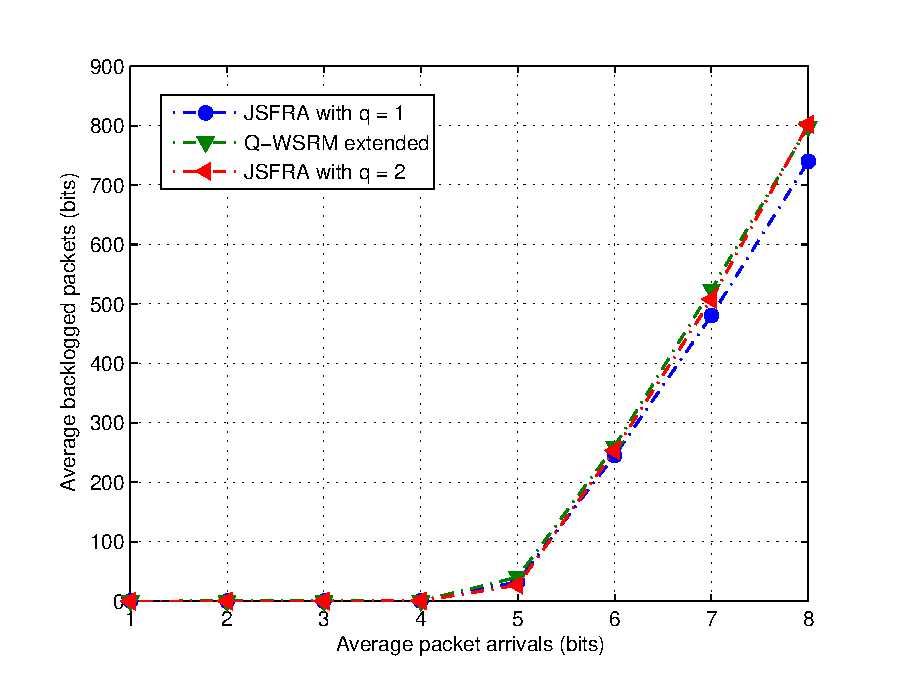
\includegraphics[width=\columnwidth]{Review/reviewer.eps}
\label{fig-review}
\caption{System \me{\lbrace N,N_B,K,N_R \rbrace = \lbrace 4,2,12,1 \rbrace}}
\end{figure}

\cmnt{2} Do the proposed solutions based on (6) achieve better average delay performance than the existing solutions? By the way, in the simulations, you should also add a figure comparing the average delay performance, instead of just comparing the performance metric defined by (6). This will better justify the advantage of the proposed solutions.

\resp We agree with the reviewer comment on the better average delay performance of Q-WSRM(E) approach over JSFRA scheme with \me{q=1} formulation. Note that the average delay can be reduced by including a convex minimum rate constraint in the JSFRA formulation to provide a guaranteed rate to all users or for certain users in the system. More over, the priority can also be incorporated easily in the formulation by the scaling factor \me{a_k} used in the formulation. As mentioned in Section \ref{sec-3.2}, the delay can also be addressed by using \me{q=2} or \me{q=\infty} norm objective in the JSFRA formulation.

\cmnt{3} In Section III.B, the convergence conditions under Algorithm 1 are not clear. First, you should be more specific about what is the SCA subproblem. Do you mean problem (19)? Second, does the uniqueness of the transmit and receive beamformers mean that the solution of the original problem in (16) is unique, or the solutions of the subproblems in (19) and (20) are unique, respectively?

\resp We understand the reviewer concerns. We have modified the convergence section to include additional information to provide more clarity. \review{Update converge proof}

\maketitle

\acused{MU-MIMO}

\begin{abstract}
We consider a multi-cell \ac{MIMO} \acl{IBC} scenario using \ac{OFDM} with \acl{MU} contending for space-frequency resources in the downlink transmission. The problem is to determine the transmit precoders by the \acp{BS} in a coordinated approach to minimize the total number of backlogged packets in the \acp{BS}, which are destined for the users in the system. Traditionally it is solved using \ac{WSRM} objective with the number of backlogged packets as the corresponding weights, \textit{i.e}, longer the queue size, higher the priority. In contrast, we design the precoders jointly across the space-frequency resources by minimizing the total user queue deviations. The problem is highly nonconvex and therefore we employ \ac{SCA} technique to solve the problem by a sequence of convex subproblems using first order Taylor approximations. At first, we discuss centralized \ac{JSFRA} solutions using the \ac{SCA} technique both in the direct formulation and also in the \ac{MSE} reformulation approach. We then propose distributed precoder designs using primal and \ac{ADMM} method for the \ac{JSFRA} solutions. Finally, we propose an iterative practical precoder design based on \ac{MSE} reformulation approach by solving the \ac{KKT} conditions. The precoders are solved using closed form expressions at each iteration. Numerical results are used to compare the proposed algorithms with the existing solutions.

%we address the queue minimizing downlink precoder design as a joint nonconvex optimization problem over space-frequency resources. We employ \ac{SCA} technique to solve the problem by a sequence of convex subproblems using inner approximations. Initially, we discuss the centralized \acl{JSFRA} solutions based on \ac{SCA} as well as by \acl{MSE} reformulation. Then we extend the distributed precoder design for the centralized schemes using primal and \ac{ADMM} method. Finally, we discuss the distributed precoder design problem by solving the \ac{KKT} expressions to obtain the closed form solutions for the transmit and the receive precoders. Numerical results are shown to compare them.



\end{abstract}

\begin{IEEEkeywords}
Convex approximations, \ac{MIMO}-\acs{IBC}, \ac{MIMO}-\ac{OFDM}, Precoder design, \acs{SCA}, \ac{WSRM}.
\end{IEEEkeywords}

\acresetall

\section{Introduction} \label{sec-1}

The last mile wireless connectivity poses significant bottleneck in the overall data traffic for the interconnected networks. The main challenges in the wireless networks are due to the scarcity of the available resources either in terms of power or spectrum usage and the complexity of the receiver algorithms which are proportional to the mobile battery drain. In order to overcome the receiver complexity, \ac{OFDM} based transmissions are introduced for the wideband transmissions. To improve data rate, multiple antennas are installed at \acp{BS} and/or at user terminals to avail additional freedom in the form of spatial dimension. The inclusion of \ac{MIMO} technique in wireless networks provides higher data rate or lower outage for the same transmission power and bandwidth.

In a network with multiple \acp{BS} serving multiple users (\acs{MU}), the main driving factor for the transmission are the packets waiting at each \ac{BS} corresponding to the different users present in the network. These available packets are transmitted over the shared wireless resources subject to certain system limitations and constraints. In this work, we consider the problem of transmit design over the space-frequency resources provided by a \ac{MU-MIMO} \ac{OFDM} framework in the downlink broadcast transmission to minimize the number of queued packets. Since the space-frequency resources are shared by multiple users associated with different \acp{BS}, the problem of interest can be viewed as a resource allocation to minimize the total number of backlogged packets of all \acp{BS}.

In general, the resource allocation problems are solved by assigning a binary variable to each user indicating the presence or the absence on a particular resource. In contrast to that, we use the transmit beamformers, which are the complex vectors, as a decision variable in determining the presence or the absence of a user on a particular resource. The purpose of using the transmit beamformers for the scheduling is two fold. Firstly, it determines the transmission rate on a certain resource and secondly, by making the transmit beamformer to be a zero vector, the corresponding user will not be scheduled on a certain resource.

In order to reduce the complexity involved in the precoder design problem, linear precoding are assumed at the \acp{BS} and linear detection is used at users. The queue minimizing network optimization objective is used to design the beamformers across the coordinating \acp{BS}, since the transmissions are guided by the available backlogged packets. To achieve the best performance, we propose a joint resource allocation scheme over the space and frequency dimensions among the coordinating \acp{BS} to minimize the time that the packets stay in the queues prior to the transmission, and, hence, to avoid packet drops as an indirect objective.

The queue minimizing precoder designs are closely related to the \ac{WSRM} problem with additional rate constraints determined by the number of backlogged packets for each user in the system (see Section \ref{sec-3} for further discussions). The topics on \ac{MIMO} \ac{BC} precoder design have been studied extensively with different performance criteria in the literature. Due to the nonconvex nature of most, if not all, linear \ac{MIMO} \ac{BC} precoder design problems, the \ac{SCA} method has gradually become a powerful tool to deal with these problems. For example, in \cite{sin_algorithm}, the nonconvex part of the objective is linearized around an operating point in order to solve the \ac{WSRM} problem in an iterative manner. Similar approach of solving the \ac{WSRM} problem via arithmetic-geometric inequality is proposed in \cite{tran2012fast}.

The connection between the achievable capacity and the \ac{MSE} for the received symbol by using the fixed \ac{MMSE} receivers as shown in \cite{viswanath1999optimal,mse_duality} is also used to solve the \ac{WSRM} problem. In \cite{christensen2008weighted,wmmse_shi}, the \ac{WSRM} problem is reformulated via \ac{MSE}, casting the problem as a convex one for fixed \ac{MMSE} receivers. In this way, the original problem is expressed in terms of the \ac{MSE} weight, precoders, and decoders. Then the problem is solved using an alternating optimization method, i.e., finding a set of variables while the remaining others are fixed. Additional rate constraints based on the \ac{QoS} requirements are included in the \ac{WSRM} problem are solved via \ac{MSE} reformulation in \cite{kaleva2013primal}.

The problem of precoder design for the \ac{MIMO} \ac{BC} system are solved either by using a centralized controller or by using decentralized algorithms where each BS handles their own problems and exchange limited information via backhaul. The distributed approaches are based on the primal or dual decomposition \cite{palomar2006tutorial,boyd2011distributed}. In primal decomposition, the so-called coupling interference variables are fixed for the subproblem at each \ac{BS} to find the optimal precoders. The fixed interference are then updated by using the subgradient method as discussed in \cite{pennanen2011decentralized}. The dual approach controls the distributed subproblems by fixing the \emph{`interference price'} for each \ac{BS} as detailed in \cite{tolli2011decentralized}.

By adjusting the weights properly, we can find arbitrary rate-tuple in the rate region of the system that maximizes other performance measures by solving the resulting WSRM problem. For example, if the weight of each user is set to be inversely proportional to his/her data rate, the corresponding problem guarantees fairness among users. As an approximate method, we may assign weights based on the current queue size of users. More specifically, the queue states can be incorporated to traditional weighted sum rate objective $\sum_k w_k R_k$ by replacing the weight $w_k$ with the corresponding queue state $Q_k$ or a function of it,  which is the outcome of minimizing the Lyapunov drift between the current and the future queue states \cite{tassiulas,neely2010stochastic}. In the backpreassure algorithm, the differential queues between the source and the destination nodes are used as the weights scaling the transmission rate \cite{georgiadis2006resource}.

Earlier studies on the queue minimization problem was summarized in the survey paper \cite{berry2004cross}. In particular, the problem of power allocation to minimize the number of backlogged packets was considered in \cite{qps_cioffi} by geometric programming formulations. Since the problem considered in \cite{qps_cioffi} assumed single antenna transmitters and receivers, the queue minimizing problem reduces to the one of optimal power allocation. In the context of wireless networks, the backpreassure algorithm mentioned above was extended in \cite{weeraddana2011resource} by formulating the corresponding user queues as the weights in the \ac{WSRM} problem.

In this paper, we consider the problem of precoder design across the space-frequency resources to minimize the total number of queued packets of all \acp{BS}. For this highly nonconvex problem, we first propose two centralized methods. In the first method, we relax the nonconvex constraint by the first order taylor approximation around an operating point, which is updated in an iterative manner until convergence or to a certain accuracy. In the second method, we reformulate the \ac{JSFRA} problem using the \ac{MSE} equivalence with the rate expression to solve for the optimal precoders. For distributed implementation, we further proposed decentralized approaches based on primal and \ac{ADMM} scheme to identify the precoders independently across the \acp{BS} by exchanging limited information via backhaul. We also proposed an iterative algorithm by solving the \ac{KKT} equations, which can be implemented easily in a distributed manner.

The remainder of this paper is as follows. In Section \ref{sec-2-3.2}, we introduce the system model and the problem formulation for the queue minimizing precoder design. Existing and the proposed precoder designs for the \ac{JSFRA} problem are presented in Section \ref{sec-3}. The distributed solutions are provided in Section \ref{sec-4} followed by the simulation results in Section \ref{sec-5}. Conclusions are drawn in Section \ref{sec-6}.

\section{System Model and Problem Formulation} \label{sec-2-3.2}
\subsection{System Model} \label{sec-2}
We consider a downlink \ac{MIMO} \ac{IBC} scenario in an \ac{OFDM} framework with \me{N} sub-channels and \me{N_B} \acp{BS} each equipped with \me{N_T} transmit antennas, serving in total \me{K} users each with \me{N_R} receive antennas. The set of users associated with \ac{BS} \me{b} is denoted by \me{\mathcal{U}_b} and the set \me{\mathcal{U}} represents all users in the system, i.e., \me{\mathcal{U} =\underset{b\in \mathcal{B}}{\cup }\mathcal{U}_b}, where \me{\mathcal{B}} is the set of indices of all coordinating \acp{BS}. Data for user \me{k} is transmitted from only one \ac{BS} which is denoted by \me{b_k\in \mathcal{B}}. Let \me{\mathcal{N} = \set{1,2,\dotsc,N}} be the set of all sub-channel indices available in the system. 

We adopt linear transmit beamforming technique at \acp{BS}. Specifically, the data symbols \me{d_{l,k,n}} for  user \me{k} on the \me{l^\mathrm{th}} spatial stream over sub-channel \me{n} is multiplied with beamformer \me{\mvec{m}{l,k,n} \in \mathbb{C}^{N_T \times 1}} before being transmitted. In order to detect  multiple spatial streams at the user terminal, receive beamforming vector \me{\mvec{w}{l,k,n}} is employed for each user. Consequently, the received data estimate corresponding to the \me{l^\mathrm{th}} spatial stream over sub-channel \me{n} at user $k$ is given by
\iftoggle{single_column}{
\begin{equation}\label{eqn-1}
\hat{d}_{l,k,n} = \mvec{w}{l,k,n}^\herm \mvec{H}{b_k,k,n} \,\mvec{m}{l,k,n} d_{l,k,n} + \mvec{w}{l,k,n}^\herm \sum_{i \in \mc{U} \backslash \set{k}} \mvec{H}{b_i,k,n} \sum_{j = 1}^L \mvec{m}{j,i,n}d_{j,i,n} + \mvec{w}{l,k,n}^\herm \mvec{n}{k,n}
\end{equation}
}{
\begin{multline}\label{eqn-1}
\hat{d}_{l,k,n} = \mvec{w}{l,k,n}^\herm \mvec{H}{b_k,k,n} \,\mvec{m}{l,k,n} d_{l,k,n} + \mvec{w}{l,k,n}^\herm \mvec{n}{k,n} \\ 
+ \mvec{w}{l,k,n}^\herm \sum_{i \in \mc{U} \backslash \set{k}} \mvec{H}{b_i,k,n} \sum_{j = 1}^L \mvec{m}{j,i,n}d_{j,i,n}
\end{multline}
}
where \me{\mvec{H}{b,k,n} \in \mathbb{C}^{N_R \times N_T}} is the channel between \ac{BS} \me{b} and  user \me{k} on sub-channel \me{n}, and \me{\mvec{n}{k,n}} \me{\sim \mc{CN}(0,N_0)} is the additive noise vector for user \me{k} on the \me{n^\mathrm{th}} sub-channel and \me{l^\mathrm{th}} spatial stream. In \eqref{eqn-1}, \me{L = \text{rank}(\mvec{H}{b,k,n}) = \min(N_T,N_R)} is the maximum number of spatial streams.\footnote{It can be easily extended for user specific streams \me{L_k} instead of using common \me{L} streams for all users. \me{L} streams are initialized but after solving the problem, only \me{L_{k,n} \leq L} non-zero data streams are transmitted.} Assuming independent detection of data streams, we can write the signal-to-interference-plus-noise ratio (SINR) as
\begin{equation}\label{eq:SINR}
\gamma_{l,k,n} = \dfrac{\left |\mvec{w}{l,k,n}^\herm \, \mvec{H}{b_k,k,n} \, \mvec{m}{l,k,n} \right |^2}{\enoise + \sum_{(j,i) \neq (l,k)} |\mvec{w}{l,k,n}^\herm \mvec{H}{b_i,k,n} \mvec{m}{j,i,n} |^2}
\end{equation}
where \me{\enoise = N_0 \, \trace (\mvec{w}{l,k,n} \mbf{w}_{l,k,n}^\herm)} denotes the equivalent noise variance. \review{To reduce the overhead involved in feeding back the user channels, we consider a \ac{TDD} system in which \acp{BS} can estimate the downlink channels from the uplink pilots using channel reciprocity.}

Let \me{Q_k} be the number of backlogged packets destined for user \me{k} at a given scheduling instant. The queue dynamics of user \me{k} are modeled using the Poisson arrival process with the average number of packet arrivals of \me{A_k = \mathbf{E}_i\{\lambda_k\}} packets/bits, where \me{\lambda_k(i) \sim \mathrm{Pois}(A_k)} represents the instantaneous number of packets arriving for user \me{k} at the \me{{i}^\mathrm{th}} time instant.\footnote{The unit can either be packets or bits as long as the arrival and the transmission units are similar.} The total number of queued packets at the \me{{(i+1)}^\mathrm{th}} instant for user \me{k}, denoted as \me{Q_k(i+1)}, is given by
\begin{equation}
Q_k(i+1) = \Big [ Q_k(i) - t_k(i) \Big ]^+ + \lambda_k(i)
\label{eqn-2a}
\end{equation}
where \me{[x]^+ \equiv \max{ \lbrace x,0  \rbrace}} and \me{t_k} denotes the number of transmitted packets or bits for user \me{k}. At the \me{\ith{i}} instant, the transmission rate of user \me{k} is given by
\begin{equation}
t_k(i) = \sum_{n = 1}^N \, \sum_{l = 1}^L \, t_{l,k,n}(i)
\end{equation}
where \me{t_{l,k,n}} denotes the number of transmitted packets or bits over the \me{\ith{l}} spatial stream on the \me{\ith{n}} sub-channel. The maximum rate achieved over the space-frequency resource \me{(l,n)} is given by \me{t_{l,k,n} \leq \log_2(1 + \gamma_{l,k,n})} for the \ac{SINR} \me{\gamma_{l,k,n}}.\footnote{The upper bound can be achieved by using Gaussian signaling.} The units of \me{t_k} and \me{Q_k} are in bits defined per channel use. 
\subsection{Problem Formulation} \label{sec-3.2}

To minimize the total number of backlogged packets, we consider minimizing weighted \me{\ell_{q}}-norm of all the queue deviation given by
\begin{equation}
v_k =  Q_k - t_k = Q_k - \sum_{n = 1}^N \sum_{l = 1}^{L} \log_2(1+\gamma_{l,k,n})
\label{eqn-4.2}
\end{equation}
Explicitly, the considered problem is given by \me{\sum_{k \in \mc{U}} \, a_k | v_k |^q}. With this objective, the problem of weighted queued packet minimization is given by
\begin{IEEEeqnarray}{rCl}\label{eqn-3}
\underset{\substack{\mvec{M}{k,n},\mvec{W}{k,n}}}{\text{minimize}} &\quad& \|  \tilde{\mbf{v}}  \|_q\IEEEyessubnumber \\
\text{subject to} & \quad&\sum_{n = 1}^N \sum_{k \in \mathcal{U}_b} \text{tr} \, (\mvec{M}{k,n} \mvec{M}{k,n}^\herm) \leq P_{{\max}}, \fall b \IEEEyessubnumber \label{eqn-4.3}
\end{IEEEeqnarray}
where \me{\tilde{v}_k \triangleq a_k^{1/{q}}v_k}, and \me{a_k} is the weighting factor which is incorporated to control user priority based on their respective \ac{QoS}, \me{\mbf{M}_{k,n} \triangleq [ \, \mvec{m}{1,k,n} \, \mvec{m}{2,k,n} \dotsc \mvec{m}{L,k,n} \,]} comprises the beamformers associated with the user \me{k} for \me{n^\mathrm{th}} sub-channel transmission, and \me{\mbf{W}_{k,n} \triangleq [ \, \mvec{w}{1,k,n} \, \mvec{w}{2,k,n} \dotsc \mvec{w}{L,k,n} \,]} stacks the receive beamformers respectively\footnote{It can be easily extended for user specific streams \me{L_{k,n}} instead of using the common \me{L} streams for all users}. In \eqref{eqn-4.3}, we consider a \ac{BS} specific sum power constraint for each \ac{BS} across all sub-channels.

For practical and tractability reasons, we may impose a constraint that the maximum number of transmitted bits for the user \me{k} is limited by the total backlogged packets available at the transmitter. As a result, the number of backlogged packets \me{v_k} remaining in the system for the user \me{k} is given by
\begin{equation} \label{rate_constraint_a}
v_k =  Q_k - \sum_{n = 1}^N \sum_{l = 1}^{L} \log_2(1+\gamma_{l,k,n}) \geq 0
\end{equation}
The above positivity constraint need to be satisfied by \me{v_k} to avoid the excessive allocation of the resources.

Before proceeding further, we note that the constraint in \eqref{rate_constraint_a} is handled implicitly by the definition of the \me{\ell_q} in the objective of \eqref{eqn-3}. As a proof, suppose that \me{t_k>Q_k} for a certain \me{k} at optimum, i.e., \me{-{v}_k=t_k-Q_k>0}. Then there exists \me{\delta_k>0} such that \me{-{v}^{\prime}_k=t^{\prime}_k-Q_k<-{v}_k} where \me{t^{\prime}_k=t_k-\delta_k}. Since \me{\|\tilde{\mbf{v}}\|_q=\| |\tilde{\mbf{v}}| \|_q=\||-\tilde{\mbf{v}}|\|_q}, this means that the newly created vector \me{\mbf{t}^{\prime}} achieves a smaller objective which contradicts with the fact that an optimal solution has been obtained. The choice of the norm \me{\ell_q} used in the objective function \cite{berry2004cross,qps_cioffi} alters the priorities for the queue deviation function as
\begin{itemize}
\item With \me{\ell_{q = 1}}, the objective results in greedy allocation \textit{i.e}, emptying the queue of users with good channel condition before considering the users with worse channel conditions. As a special case, it is easy to see that \eqref{eqn-3} reduces to the \ac{WSRM} problem \eqref{gen_sum} when the queue size is large enough for all users.
\item With \me{\ell_{q = 2}}, the objective prioritizes users with higher number of queued packets before considering the users with a smaller number of backlogged packets. For example, it could be more ideal for the delay limited scenario when the packet arrival rates of the users are similar, since the backlogged packets is proportional to the delay in the transmission following the Little's law \cite{neely2010stochastic}.
\item With \(\ell_{q = \infty} \), the objective minimizes the maximum number of queued packets among users with the current transmission, thereby providing queue fairness by allocating the resources proportional to the number of backlogged packets.
\end{itemize} 

\section{Proposed Queue Minimizing Precoder Designs} \label{sec-3}

In this section, we discuss the precoder design solutions for the problem stated in Section \ref{sec-3.2}. To begin with, we discuss the existing solution and its extension to solve the current problem of resource allocation over multiple sub-channels. Then, we provide two different approaches to solve the \ac{JSFRA} precoder design problem to minimize the total number of backlogged packets. At the end of the section, we discuss a low complex solution for the \ac{JSFRA} problem by limiting the precoder design over each sub-channel at a given instant.

In general, the precoder design for the \ac{MIMO} \ac{OFDM} problem is highly difficult due to the combinatorial and the non-convex nature of the problem. In addition to that, the objective of minimizing the number of the queued packets over the spatial and the sub-channel dimensions adds further complexity to the existing problem. Since the scheduling of users in each sub-channel can be made by allocating zero transmit power over certain sub-channels, the solutions provided in the paper performs both precoder design and the scheduling of users in a joint manner.

\subsection{Queue Weighted Sum Rate Maximization (\acs{Q-WSRM}) Formulation} \label{sec-3.1}

The queue minimizing algorithms are discussed extensively in the networking literature to provide congestion-free routing between any two nodes in the network. One such algorithm  is the \emph{backpressure algorithm} \cite{tassiulas,georgiadis2006resource,neely2010stochastic}. It determines an optimal control policy in the form of rate or resource allocation for the nodes in the network by considering the differential backlogged packets between the source and the destination nodes. Even though the algorithm is primarily designed for the wired infrastructure, it can be extended to the wireless networks by designing the user rate variable \me{t_k} in accordance to the wireless network.

The \ac{Q-WSRM} formulation extends the \emph{backpressure algorithm} to the \ac{MIMO}-\ac{OFDM} downlink framework, in which the multiple \acp{BS} act as the source nodes and the user terminals as the receiver nodes. The control policy in the form of transmit precoders is designed to minimize the number of queued packets waiting at the \acp{BS}. In order to find the optimal algorithm, we use the Lyapunov function which is predominantly used in the control theory for the system stability. Since at each time slot, the system can be described by the channel conditions and the number of backlogged packets of each user, the Lyapunov function is used to provide a scalar measure, which grows large when the system moves toward the undesirable state. Following the approach in \cite{neely2010stochastic}, the scalar measure for the queue stability is given by
\begin{equation}
\mathrm{L}\sset{\mbf{Q}(i)} = \frac{1}{2} \, \sum_{k \in \mc{U}} Q_k^2(i),
\end{equation}
where \me{\mbf{Q}(i)} denotes the stacked user queues at the \me{\ith{i}} slot and \me{\frac{1}{2}} is used for the convenience. The Lyapunov function provides a measure of congestion in the system, as discussed in \cite[Ch. 3]{neely2010stochastic}. The Lyapunov function drift, expressed as \me{\mathrm{L}\sset{\mbf{Q}(i+1)} - \mathrm{L}\sset{\mbf{Q}(i)}}, is given by 
\begin{IEEEeqnarray}{rCl}\label{eqn-3.1}
&=&\frac{1}{2} \Big [ \sum_{k \in \mc{U}} \, \Big ( \left [ Q_k(i) - t_k(i) \right ]^+ + \lambda_k(i) \Big )^2 - Q^2_k(i) \Big ] \IEEEyessubnumber \label{eqn-3.1.0} \\
&\leq& \sum_{k \in \mc{U}} \, \frac{\lambda^2_k(i) + t_k^2(i)}{2} + \sum_{k \in \mc{U}} Q_k(i) \set{ \lambda_k(i) - t_k(i) }, \IEEEyessubnumber \label{drift-exp}
\end{IEEEeqnarray}
where the inequality is due to the upper bound
\begin{equation}
\sset{\max(Q-t,0) + \lambda)}^2 \leq Q^2 + t^2 + \lambda^2 + 2 Q (\lambda - t).
\end{equation}
The total number of backlogged packets at any given instant \me{i} is reduced by minimizing the conditional expectation of the Lyapunov drift expression \eqref{drift-exp} given the current number of queued packets \me{\mbfa{Q}(i)} waiting in the system. The expectation is taken over all possible arrival and transmission rates of the users to obtain the optimal rate allocation strategy. 

Now, the conditional Lyapunov drift, denoted by \me{\Delta{(\mbfa{Q}(i))}}, is given by
\iftoggle{single_column}{
\begin{IEEEeqnarray}{rCl} \label{backpressure-approx}
	\underset{\mbf{t}}{\text{minimize}} && \Delta(\mbf{Q}(i)) \triangleq \mathbb{E}_{\mbfa{\lambda},\mbf{t}} \set{\mathrm{L}\sset{\mbf{Q}(i+1)} - \mathrm{L}\sset{\mbf{Q}(i)} \vert \mbf{Q}(i)} \IEEEyessubnumber \\
	&\leq& \underbrace{\mathbb{E}_{\mbfa{\lambda},\mbf{t}} \set {\sum_{k \in \mc{U}} \, \frac{\lambda^2_k(i) + t_k^2(i)}{2} \vert \mbf{Q}(i)}}_{\le B} + \sum_{k \in \mc{U}} Q_k(i) A_k(i) - \mathbb{E}_{\mbfa{\lambda},\mbf{t}}\set{\sum_{k \in \mc{U}} Q_k(i) t_k(i)  \vert \mbf{Q}(i)}, \IEEEyessubnumber \label{backpreassure-approx-1b}
\end{IEEEeqnarray}}{
{\allowdisplaybreaks
\begin{IEEEeqnarray}{CL} \label{backpressure-approx}
	& \underset{\mbf{t}}{\text{minimize}} \quad \mathbb{E}_{\mbfa{\lambda},\mbf{t}} \set{\mathrm{L}\sset{\mbf{Q}(i+1)} - \mathrm{L}\sset{\mbf{Q}(i)} \vert \mbf{Q}(i)} \IEEEyessubnumber \\
	\leq & \underbrace{\mathbb{E}_{\mbfa{\lambda},\mbf{t}} \Big \lbrace \sum_{k \in \mc{U}} \frac{\lambda^2_k(i) + t_k^2(i)}{2} \vert \mbf{Q}(i) \Big \rbrace }_{\le B} + \sum_{k \in \mc{U}} Q_k(i) A_k(i) \nonumber \\
	& \qquad \qquad {} - \mathbb{E}_{\mbfa{\lambda},\mbf{t}}\Big \lbrace \sum_{k \in \mc{U}} Q_k(i) t_k(i)  \vert \mbf{Q}(i) \Big \rbrace, \IEEEyessubnumber \label{backpreassure-approx-1b}
\end{IEEEeqnarray}}}
%\begin{figure*}
%\begin{IEEEeqnarray}{rCl} \label{backpressure-approx}
%	\underset{\mbf{t}}{\text{minimize}} &\quad& \mathbb{E}_{\mbfa{\lambda},\mbf{t}} \set{\mathrm{L}\sset{\mbf{Q}(i+1)} - \mathrm{L}\sset{\mbf{Q}(i)} \vert \mbf{Q}(i)} \IEEEyessubnumber \vspace{-0.25in}\\
%	& \leq & \sum_{k \in \mc{U}} Q_k(i) A_k(i) - \mathbb{E}_{\mbfa{\lambda},\mbf{t}}\set{\sum_{k \in \mc{U}} Q_k(i) t_k(i)  \vert \mbf{Q}(i)} + \overbrace{\mathbb{E}_{\mbfa{\lambda},\mbf{t}} \set {\sum_{k \in \mc{U}} \frac{\lambda^2_k(i) + t_k^2(i)}{2} \vert \mbf{Q}(i)}}^{\le B}\IEEEyessubnumber \label{backpreassure-approx-1b}
%\end{IEEEeqnarray}	
%\vspace{-0.25in}
%\end{figure*}
where the first term in \eqref{backpreassure-approx-1b} follows from the Poisson arrival process. Since the transmission and the arrival rates are bounded, we can upper bound the second order moments in the first term of \eqref{backpreassure-approx-1b} by a constant \me{B} that can be eliminated from the optimization problem \cite{neely2010stochastic}.

The expression in \eqref{backpressure-approx} looks similar to the \ac{WSRM} formulation if the weights in the \ac{WSRM} problem are replaced by the number of backlogged packets corresponding to the users. The above discussed approach is extended for the wireless networks in \cite{weeraddana2011resource}, where the queue weighted sum rate maximization is considered as the objective function to determine the transmit precoders. Since the expectation can be minimized by minimizing the function inside, the \ac{Q-WSRM} formulation is given by 
\begin{IEEEeqnarray}{rCl} \label{q_gen_sum}
	\underset{\substack{\mvec{M}{k,n}, \mvec{W}{k,n}}}{\text{maximize}} &\quad& \sum_{k \in \mc{U}} \, Q_k \left ( \sum_{n = 1}^N \sum_{l=1}^L \log_2(1 + \gamma_{l,k,n}) \right ) \IEEEyessubnumber \label{eqn-3.1.1} \\
	\text{subject to.} & \quad & \sum_{n = 1}^N \sum_{k \in \mathcal{U}_b} \text{tr} \, (\mvec{M}{k,n} \mvec{M}{k,n}^\herm) \leq P_{{\max}}, \fall b \IEEEyessubnumber \label{eqn-3.1.3}
\end{IEEEeqnarray}
In order to avoid the excessive  allocation of the resources, we include an additional rate constraint \me{t_k \leq Q_k} to address \me{[x]^+} operation in \eqref{eqn-2a}. The rate constrained version of the \ac{Q-WSRM}, denoted by \ac{Q-WSRME} problem for a cellular system, is given by \label{q_gen_sum-1} with the additional constraint
\begin{IEEEeqnarray}{rCl} \label{eqn-3.1.4}
\sum_{n=1}^N \sum_{l = 1}^L \log_2(1 + \gamma_{l,k,n}) \leq Q_k, \fall k \in \mc{U}
\end{IEEEeqnarray}
where the precoders are associated with the \me{\gamma_{l,k,n}} defined in \eqref{eq:SINR}. By using the number of queued packets as the weights, the resources can be allocated to the user with the more number of backlogged packets, which essentially does the allocation in a greedy manner.

As a special case of the problem defined in \eqref{q_gen_sum}, we can formulate the sum rate maximization problem by setting the weights in \eqref{eqn-3.1.1} as unity, leading to the problem as in \eqref{q_gen_sum} with \me{Q_k = 1, \forall k \in \mc{U}}. This approach provides a greedy queue minimizing allocation as compared to \ac{Q-WSRME}, since the resource allocation is driven by the channel conditions in comparison with the number of queued packets as in \ac{Q-WSRME}. Note that in both formulations, the resources allocated to the users are limited by the backlogged packets with an explicit maximum rate constraint defined by \eqref{eqn-3.1.4}.


\subsection{\acs{JSFRA} Scheme via \ac{SCA} approach} \label{sec-3.2.1}
The problem defined in \eqref{q_gen_sum} ignores the second order term arising from the Lyapunov drift minimization objective by limiting it to a constant value. \review{In fact, using \me{\ell_{q=2}} in \eqref{eqn-4.2}, we obtain the following objective
\begin{equation}\label{pf-1}
\underset{t_k}{\text{minimize}} \, \sum_k \, v_k^2 = \underset{t_k}{\text{minimize}} \, \sum_k \, Q_k^2 - 2 \, Q_k t_k + t_k^2
\end{equation}
which is similar to the objective in \eqref{q_gen_sum}. It is achieved either by removing \me{t_k^2} from \eqref{pf-1} or when the total number of queued packets is large for all users such that \me{t_k^2} has no impact on the objective function.}

By limiting \me{t_k^2} with a constant value, the \ac{Q-WSRM} formulation requires an explicit rate constraint \eqref{eqn-3.1.4} to avoid over-allocation of the available resources. In the proposed queue deviation formulation, the explicit rate constraint is not needed, since it is handled by the objective function \eqref{eqn-4.2} itself. It makes the problem simpler and allows us to employ efficient algorithms to distribute the precoder design problem across each \ac{BS} independently with minimal information exchange \cite{boyd2011distributed}. In contrast to the \ac{WSRM} formulation, the \ac{JSFRA} and the \ac{Q-WSRME} problems handle the sub-channels jointly to obtain an efficient allocation by identifying the optimal space-frequency resources for the users.

In this approach, we present an algorithm to solve \eqref{eqn-3} to obtain the transmit precoders in a centralized manner by using the idea of alternating optimization and successive convex approximation. Using \eqref{eq:SINR}, we can reformulate the problem defined in \eqref{eqn-3} as
\iftoggle{single_column}{
\begin{IEEEeqnarray}{CCl}\label{eqn-6}
\underset{\substack{\gamma_{l,k,n},\mvec{m}{l,k,n},\\ \beta_{l,k,n},\mvec{w}{l,k,n}}}{\text{minimize}} & \quad & \|  \tilde{\mbf{v}}  \|_q \label{eqn-obj} \IEEEyessubnumber \\
\text{subject to}& \quad &\gamma_{l,k,n} \leq \frac{ | \mvec{w}{l,k,n}^\herm \mvec{H}{l,k,n} \mvec{m}{l,k,n}  |^2}{\beta_{l,k,n}} \triangleq f(\tilde{\mbf{u}}_{l,k,n}) \IEEEyessubnumber \label{eqn-6.2} \\
  & \quad & \beta_{l,k,n} \geq  \tilde{N}_0 + \hspace{-0.75em} \sum_{(j,i) \neq (l,k)} \hspace{-0.75em} |\mvec{w}{l,k,n}^\herm \mvec{H}{b_i,k,n} \mvec{m}{j,i,n} |^2 \IEEEyessubnumber \label{eqn-6.3} \\
  & \quad & \text{and } \eqref{eqn-4.3}, \IEEEyessubnumber
\end{IEEEeqnarray}
}{\allowdisplaybreaks
\begin{IEEEeqnarray}{CCl}\label{eqn-6}
	\underset{\substack{\gamma_{l,k,n},\mvec{m}{l,k,n},\\\beta_{l,k,n},\mvec{w}{l,k,n}}}{\text{minimize}} &\quad& \|  \tilde{\mbf{v}}  \|_q \label{eqn-obj} \IEEEyessubnumber \vspace{-0.25cm}\\
	\text{subject to} &\quad& \gamma_{l,k,n} \leq \frac{ | \mvec{w}{l,k,n}^\herm \mvec{H}{l,k,n} \mvec{m}{l,k,n}|^2}{\beta_{l,k,n}} \triangleq f(\tilde{\mbf{u}}_{l,k,n}) \IEEEyessubnumber \eqspace \label{eqn-6.2} \\
	&\quad& \beta_{l,k,n} \geq \tilde{N}_0 + \sum_{\mathclap{(j,i) \neq (l,k)}} |\mvec{w}{l,k,n}^\herm \mvec{H}{b_i,k,n} \mvec{m}{j,i,n} |^2 \IEEEyessubnumber \eqspace \label{eqn-6.3} \\
	&\quad& \text{and } \eqref{eqn-4.3}, \IEEEyessubnumber
\end{IEEEeqnarray}
}
where \me{\tilde{\mbf{u}}_{l,k,n} \triangleq \{\mvec{w}{l,k,n}^\herm, \mvec{H}{b_k,k,n}, \mvec{m}{l,k,n},\beta_{l,k,n}\}} is the vector which needs to be identified for the optimal allocation and \me{\tilde{N}_0 = N_0\|\mvec{w}{l,k,n}\|^2} be the effective noise variance. In this formulation, we relaxed the equality constraint in \eqref{eq:SINR} by the inequalities in \eqref{eqn-6.2} and \eqref{eqn-6.3}. However, this step leads to the same solution without loss of optimality, since the inequalities in \eqref{eqn-6.2} and \eqref{eqn-6.3} are active for an optimal solution, following the same arguments as those in \cite{tran2012fast}. Intuitively, \eqref{eqn-6.2} denotes the \ac{SINR} constraint for \me{\gamma_{l,k,n}}, and \eqref{eqn-6.3} gives an upper bound for the total interference seen by user \me{k \in \mathcal{U}_b}, denoted by variable \me{\beta_{l,k,n}}. Similar to the \ac{WSRM} problem in \cite{tran2012fast}, the problem can be shown to be NP-hard even for the single antenna case. The reformulation in \eqref{eqn-6} allows a tractable solution as presented below. First, we note that the constraints \eqref{eqn-4.3} are convex with involved variables. Thus, we only need to deal with \eqref{eqn-6.2} and \eqref{eqn-6.3}. Towards this end, we resort to the traditional coordinate descent technique by fixing the linear receivers, and finding the optimal transmit beamformers. Recall that the coordinate descent method assumes that the optimization variables belong to disjoint sets and the problem is convex for a variable while all other variables are fixed \cite{xu2013block}.

By fixing the receivers, the problem now is to find the optimal transmit beamformers for a given set of linear receivers which is still a challenging task. We note that for fixed \me{\mvec{w}{l,k,n}}, \eqref{eqn-6.3} can be written as a \ac{SOC} constraint. Thus, the difficulty is due to the non-convexity in \eqref{eqn-6.2}. To arrive at a tractable formulation, we adopt the \ac{SCA} method to handle \eqref{eqn-6.2} by replacing the original non-convex constraint by a series of convex constraints. Note that function \me{f(\tilde{\mbf{u}}_{l,k,n})} in \eqref{eqn-6.2} is convex for fixed \me{\mvec{w}{l,k,n}}, since it is in fact the ratio between a quadratic form of \me{\mvec{m}{l,k,n}} over an affine function of \me{\beta_{l,k,n}} \cite{boyd2004convex}. According to the \ac{SCA} method, we relax \eqref{eqn-6.2} to a convex constraint in each iteration of the iterative procedure. Since \me{f(\tilde{\mbf{u}}_{l,k,n})} is convex, a concave approximation of \eqref{eqn-6.2} can be easily found by considering the first order approximation of \me{f(\tilde{\mbf{u}}_{l,k,n})} around the current operation point. For this purpose, let the real and imaginary component of the complex number \me{\mvec{w}{l,k,n}^\herm \mvec{H}{b_k,k,n} \mvec{m}{l,k,n}} be represented by
\begin{subeqnarray} \label{eqn-wsrm-expr}
p_{l,k,n} &\triangleq& \Re \set{{\mvec{w}{l,k,n}^\herm \mvec{H}{b_k,k,n} \mvec{m}{l,k,n}}} \\
q_{l,k,n} &\triangleq& \Im \set{{\mvec{w}{l,k,n}^\herm \mvec{H}{b_k,k,n} \mvec{m}{l,k,n}}}
\end{subeqnarray}
and hence \me{f(\tilde{\mbf{u}}_{l,k,n})=(p_{l,k,n}^2 + q_{l,k,n}^2)/\beta_{l,k,n}}\footnote{Note that \me{p_{l,k,n}} and \me{q_{l,k,n}} are just symbolic notation and not the newly introduced optimization variables. In CVX \cite{grant2008cvx}, for example,  we declare \me{p_{l,k,n}} and \me{q_{l,k,n}} with the `\emph{expression}' qualifier}. Suppose that the current value of \me{p_{l,k,n}} and \me{q_{l,k,n}} at a specific iteration are \me{\tilde{p}_{l,k,n}} and \me{\tilde{q}_{l,k,n}}, respectively. Using the first order Taylor approximation around the local point \me{ [ \, \tilde{p}_{l,k,n},\tilde{q}_{l,k,n},\tilde{\beta}_{l,k,n} \, ]^T}, we can approximate \eqref{eqn-6.2} by the following linear inequality constraint as
\iftoggle{single_column}{
\begin{equation}\label{eqn-8}
	2 \frac{\tilde{p}_{l,k,n}}{\tilde{\beta}_{l,k,n}} \left ( p_{l,k,n} - \tilde{p}_{l,k,n} \right ) + 2 \frac{\tilde{q}_{l,k,n}}{\tilde{\beta}_{l,k,n}} \left ( q_{l,k,n} - \tilde{q}_{l,k,n} \right ) + \frac{\tilde{p}_{l,k,n}^2 + \tilde{q}^2_{l,k,n}}{\tilde{\beta}_{l,k,n}} \left (1 - \frac{\beta_{l,k,n} - \tilde{\beta}_{l,k,n}}{\tilde{\beta}_{l,k,n}} \right ) \geq \gamma_{l,k,n}.
\end{equation}
}{
\begin{multline}\label{eqn-8}
2 \frac{\tilde{p}_{l,k,n}}{\tilde{\beta}_{l,k,n}} \left ( p_{l,k,n} - \tilde{p}_{l,k,n} \right ) + 2 \frac{\tilde{q}_{l,k,n}}{\tilde{\beta}_{l,k,n}} \left ( q_{l,k,n} - \tilde{q}_{l,k,n} \right ) \\
+ \frac{\tilde{p}_{l,k,n}^2 + \tilde{q}^2_{l,k,n}}{\tilde{\beta}_{l,k,n}} \left (1 - \frac{\beta_{l,k,n} - \tilde{\beta}_{l,k,n}}{\tilde{\beta}_{l,k,n}} \right ) \geq \gamma_{l,k,n}.
\end{multline}
}
In summary, for the fixed linear receivers, the \ac{JSFRA} problem to find transmit beamformers is shown by
\begin{IEEEeqnarray}{CCl}\label{eqn-9}
\underset{\substack{\mvec{m}{l,k,n},\\ \gamma_{l,k,n},,\beta_{l,k,n}}}{\text{minimize}} &\quad & \| \tilde{\mbf{v}} \|_q \IEEEyessubnumber\label{eqn-9.1a} \vspace{-0.15cm} \\
\text{subject to} & \quad & \beta_{l,k,n} \geq  \tilde{N}_0 + \hspace{-0.75em} \sum_{(j,i) \neq (l,k)} \hspace{-0.75em} |\mvec{w}{l,k,n}^\herm \mvec{H}{b_i,k,n} \mvec{m}{j,i,n} |^2 \IEEEyessubnumber \eqspace \label{eqn-9.1c} \\
& \quad&\sum_{n = 1}^N \sum_{k \in \mathcal{U}_b} \text{tr} \, (\mvec{M}{k,n} \mvec{M}{k,n}^\herm) \leq P_{{\max}}, \fall b \IEEEyessubnumber \label{eqn-9.1d} \\
& \quad & \text{and } \eqref{eqn-8}. \IEEEyessubnumber \label{eqn-9.1e}
\end{IEEEeqnarray}

Now, the optimal linear receivers for the fixed transmit precoders \me{\mbf{m}_{j,i,n} \, \forall i \in \mc{U}, \, \forall n \in \mc{C}} are obtained by minimizing \eqref{eqn-3} with respect to \me{\mbf{w}_{l,k,n}} as
\begin{IEEEeqnarray}{CCl}\label{eqn-9--1}
\underset{\substack{\gamma_{l,k,n},\mvec{w}{l,k,n},\beta_{l,k,n}}}{\text{minimize}} &\quad & \| \tilde{\mbf{v}} \|_q \IEEEyessubnumber\label{eqn-9--1.1a} \\
\text{subject to} & \quad & \eqref{eqn-9.1c}, \eqref{eqn-9.1d}, \eqref{eqn-9.1e}, \text{ and } \eqref{eqn-8} \IEEEyessubnumber \label{eqn-9--1.1b}.
\end{IEEEeqnarray}
Solving \eqref{eqn-9--1} using the \ac{KKT} conditions, we obtain the following iterative expression for the receiver \me{\mvec{w}{l,k,n}} as
\begin{IEEEeqnarray}{rCl}
\mvec{\widetilde{R}}{l,k,n} &=& \displaystyle \sum_{\mathclap{(j,i)\neq (l,k)}} \mvec{H}{b_i,k,n} {\mbf{m}}_{j,i,n} {\mbf{m}}_{j,i,n}^\herm \mvec{H}{b_i,k,n}^\herm + N_0 \, \mathbf{I}_{N_R} \IEEEyessubnumber \\
\mvec{w}{l,k,n}^{(i)} &=& \left ( \tfrac{\tilde{\beta}_{l,k,n} {\mbf{m}}_{l,k,n}^\herm \mvec{H}{b_k,k,n}^\herm \mbf{w}_{l,k,n}^{(i-1)} }{\|\mvec{w}{l,k,n}^{(i-1)} \mvec{H}{b_k,k,n} {\mbf{m}}_{l,k,n} \|^2} \right )\mvec{\widetilde{R}}{l,k,n}^{-1}\mvec{H}{b_k,k,n} {\mbf{m}}_{l,k,n}, \IEEEyessubnumber \eqspace \label{opt-rx}
\end{IEEEeqnarray}
where \me{\mvec{w}{l,k,n}^{(i-1)}} is the receive beamformer from the earlier iteration, upon which the linear relaxation is performed for the nonconvex constraint in \eqref{eqn-9--1}. Note that \eqref{opt-rx} is obtained by iterating over the fixed \me{\mvec{w}{l,k,n}^{(i-1)}} at each \ac{SCA} iteration until convergence or for fixed number of iterations. It can be seen that the optimal receiver expression in \eqref{opt-rx} is in fact a scaled version of the \ac{MMSE} receiver, which is given by
\begin{IEEEeqnarray}{rCl}
\mvec{R}{l,k,n} &=& \displaystyle \sum_{i\in \mc{U}} \sum_{j=1}^L \mvec{H}{b_i,k,n} \mvec{m}{j,i,n} \mvec{m}{j,i,n}^\herm \mvec{H}{b_i,k,n}^\herm + N_0 \, \mathbf{I}_{N_R} \IEEEyessubnumber \eqspace \\
\mvec{w}{l,k,n} &=& \mathbf{R}^{-1}_{l,k,n} \; \mvec{H}{b_k,k,n} \; \mvec{m}{l,k,n}. \IEEEyessubnumber \label{eqn-10}
\end{IEEEeqnarray}

The proposed algorithm is referred to as \acl{QM} \ac{JSFRA} scheme with a per \ac{BS} power constraint, and it is outlined in Algorithm \ref{algo-1}. The iterative procedure repeats until the improvement on the objective is less than a predetermined tolerance parameter or the maximum number of iterations is reached. Instead of initializing \me{\tilde{\mbf{u}}_{l,k,n}} arbitrarily to a feasible point, transmit precoders can also be initialized with any feasible point \me{\tilde{\mbf{m}}_{l,k,n}}, which is then used to find \me{\tilde{\mbf{u}}_{l,k,n}} in an efficient manner as briefed in Algorithm \ref{algo-1}. For a fixed receive beamformer \me{\mvec{w}{l,k,n}}, the \ac{SCA} iteration is carried out until convergence or for the predefined iterations, say, \me{J_{\max}} for the optimal transmit precoders \me{\mvec{m}{l,k,n}}. Next, the receive beamformers are updated based on either \eqref{opt-rx} or \eqref{eqn-10} using the fixed transmit precoders \me{\mvec{m}{l,k,n}}. This procedure is carried out until convergence of the queue deviation or for fixed number of iterations by \me{I_{\max}} as outlined in Algorithm \ref{algo-1}.
{\allowdisplaybreaks
\begin{algorithm}
 \SetAlgoLined
 \DontPrintSemicolon
 \BlankLine
 \SetKwInput{KwInit}{Initialize}
 \KwIn{\me{a_k, \, Q_k, \, \mvec{H}{b,k,n},\; \fall b \in \mathcal{B}, \, \fall k \in \mathcal{U}, \fall n \in \mathcal{N}}}
 \KwOut{\me{\mvec{m}{l,k,n}} and \me{\mvec{w}{l,k,n} \fall l \in \set{1,2,\dotsc,L}}}
 \KwInit{\me{i=0} and transmit precoders \me{\tilde{\mbf{M}}_{k,n}} randomly satisfying the total power constraint \eqref{eqn-4.3}}
 update \me{\mvec{W}{k,n}} and \me{\tilde{\mbf{u}}_{l,k,n}} using \eqref{eqn-10} and \eqref{eqn-8} using \me{\tilde{\mbf{M}}_{k,n}}\;
 \Repeat{Queue convergence or \me{i \geq I_{\max}}}{
 initialize \me{j = 0}\;
 \Repeat{\ac{SCA} convergence or \me{j \geq J_{\max}}}{
 solve for the transmit precoders \me{\mvec{m}{l,k,n}} using \eqref{eqn-9}\;
 update the constraint set \eqref{eqn-8} with \me{\tilde{\mbf{u}}_{l,k,n}} and \me{\mvec{m}{l,k,n}} using \eqref{eqn-wsrm-expr}\;
 $j = j + 1$\;
 }
 update the receive beamformers \me{\mvec{w}{l,k,n}} using \eqref{eqn-9--1} or \eqref{eqn-10} with the updated precoders \me{\mvec{m}{l,k,n}}\;
 $i = i + 1$\;
 }
 \caption{Algorithm of \acs{JSFRA} scheme}
 \label{algo-1}
\end{algorithm}
}
\subsubsection*{Convergence}

In order to prove the convergence of the proposed iterative algorithm, following conditions are to be satisfied \cite{scutari}
\begin{itemize}
	\item convergence of the \ac{SCA} subproblem	
	\item uniqueness of the transmit and the receive beamformers
	\item monotonic convergence of the objective function
\end{itemize}
In the proposed solution, we replaced \eqref{eqn-6.2} by a convex constraint using the first order approximation, which is majorized by the quadratic-over-linear function in \eqref{eqn-6.2} from below around a fixed point \me{\tilde{\mbf{u}}^{(i)}_{l,k,n}}. Since the \ac{SCA} method is adopted in the proposed algorithm, the constraint approximation satisfies the following conditions as in \cite{marks1978technical}
\begin{subeqnarray} \label{sca-req}
	f(\tilde{\mbf{u}}_{l,k,n}) &\leq& \bar{f}(\tilde{\mbf{u}}_{l,k,n},\tilde{\mbf{u}}^{(i)}_{l,k,n}) \\
	f(\tilde{\mbf{u}}^{(i)}_{l,k,n}) &=& \bar{f}(\tilde{\mbf{u}}^{(i)}_{l,k,n},\tilde{\mbf{u}}^{(i)}_{l,k,n}) \\
	\nabla f(\tilde{\mbf{u}}^{(i)}_{l,k,n}) &=& \nabla \bar{f}(\tilde{\mbf{u}}^{(i)}_{l,k,n},\tilde{\mbf{u}}^{(i)}_{l,k,n}),
\end{subeqnarray}
where \me{\bar{f}(\mbf{x},\mbf{x}^{(i)})} is the approximate function of \me{f(\mbf{x})} around the point \me{\mbf{x}^{\ast(i)}}. The stationary point of the relaxed convex problem satisfies the \ac{KKT} conditions of the original nonconvex problem, which can be obtained by using conditions in \eqref{sca-req}. It can be seen that the  \ac{SCA} relaxed formulation converges to a local stationary point at each iteration.

The uniqueness of the transmit and the receive beamformers can be justified by forcing one antenna to be real valued to exclude the phase ambiguity arising from the complex precoders. The monotonic convergence of the objective function can be justified by the following arguments. At each \ac{SCA} iteration, the relaxed subproblem is solved for the locally optimal transmit precoders to minimize the objective function. Since the \ac{SCA} subproblem is relaxed around the \me{\ith{i-1}} optimal point, \textit{i.e},  \me{\mbf{x}^{\ast(i-1)}} for the \me{\ith{i}} iteration, the domain of the problem in the \me{\ith{i}} step includes optimal point from the  \me{\ith{i-1}} iteration as well. Therefore, at each \ac{SCA} step, the objective function can either be equal to or smaller than the previous value, thereby leading to the monotonic convergence of the objective function.

Once the problem is converged to a stationary transmit precoders, the receive beamformers are updated based on the receivers in \eqref{opt-rx} or \eqref{eqn-10}. The monotonic nature of the objective function is preserved by the receive beamformer update, since the receiver minimizes the objective value for the fixed transmit precoders, and hence the proposed \ac{JSFRA} scheme is guaranteed to converge to a stationary point of the original nonconvex problem.


\subsection{\ac{JSFRA} Scheme via \ac{MSE} Reformulation} \label{sec-3.3}

In this section, we solve the \ac{JSFRA} problem by exploiting the equivalence between the \ac{MSE} and the achievable capacity for the receivers designed based on the \ac{MMSE} criterion \cite{viswanath1999optimal,mse_duality}. The \ac{MSE} for the data symbol, represented as \me{\epsilon_{l,k,n}}, is given by
\begin{subeqnarray} \label{mse-error}
\epsilon_{l,k,n} &=& \mathbb{E} \big [ ( d_{l,k,n} - \hat{d}_{l,k,n} )^2 \big ] \\
 &=&  \left | 1 - \mvec{w}{l,k,n}^\herm \mvec{H}{b_k,k,n} \mvec{m}{l,k,n} \right |^2 + \sum_{\mathclap{(j,i) \neq (l,k)}} \left | \mvec{w}{l,k,n}^\herm \mvec{H}{b_i,i,n} \mvec{m}{j,i,n} \right |^2 + N_0 \, \|\mvec{w}{l,k,n}\|^2
\end{subeqnarray}
where \me{\mvec{m}{l,k,n}, \mvec{w}{l,k,n}} denotes the transmit and the receive beamformer and \me{\hat{d}_{l,k,n}} is the received symbol as in \eqref{eqn-1}. Now, replacing the receive beamformer in \eqref{mse-error} with the \ac{MMSE} receiver shown in \eqref{eqn-10}, we obtain the following relation between the \ac{MSE} and the \ac{SINR} as
\begin{equation} \label{eqn-mse-eq}
\epsilon_{l,k,n} = \dfrac{1}{1 + \gamma_{l,k,n}}
\end{equation}
where \me{\gamma_{l,k,n}} is the received \ac{SINR} as in \eqref{eq:SINR}. Using the equivalence in \eqref{eqn-mse-eq}, the \ac{WSRM} objective can be reformulated as the \ac{WMMSE} equivalent to obtain the precoders for the \acs{MU}-\acs{MIMO} scenario as discussed in \cite{christensen2008weighted,wmmse_shi,hong2012decomposition}.

Let \me{{v}^{\prime}_k = Q_k - \sum_{n=1}^N \sum_{l=1}^L t_{l,k,n}} denote the queue deviation corresponding to the user \me{k} and \me{\tilde{{v}}^{\prime}_k \triangleq a_k^{1/{q}}v^{\prime}_k} represents the weighted equivalent. Now, using the \ac{MSE} relation, \eqref{eqn-6} is written as
\begin{IEEEeqnarray}{LL}\label{eqn-mse-1}
\underset{\substack{t_{l,k,n},\mvec{m}{l,k,n},\\ \epsilon_{l,k,n},\mvec{w}{l,k,n}}} {\text{minimize}} & \quad \|  \tilde{\mbf{v}}^{\prime}  \|_q \IEEEyessubnumber \label{eqn-mse-1.1} \\
\text{subject to} & \quad t_{l,k,n} \leq -\log_2(\epsilon_{l,k,n}) \IEEEyessubnumber \label{eqn-mse-1.2} \\
 & \quad \epsilon_{l,k,n} \geq  \left | 1 - \mvec{w}{l,k,n}^\herm \mvec{H}{b_k,k,n} \mvec{m}{l,k,n} \right |^2 + \sum_{\mathclap{(j,i) \neq (l,k)}} \left | \mvec{w}{l,k,n}^\herm \mvec{H}{b_i,i,n} \mvec{m}{j,i,n} \right |^2 + N_0 \, \|\mvec{w}{l,k,n}\|^2 \IEEEyessubnumber \label{eqn-mse-1.3} \\
& \quad \text{and} \; \eqref{eqn-4.3}  \IEEEyessubnumber \label{eqn-mse-1.4}
\end{IEEEeqnarray}
where \eqref{eqn-mse-1.3} bounds the \ac{MSE} by \me{\epsilon_{l,k,n}} and \eqref{eqn-mse-1.2} relaxes the transmitted rate \me{{t}_{l,k,n}} using the \ac{MSE} relation.

The \acl{QM} \ac{JSFRA} problem using alternative \ac{MSE} formulation given by \eqref{eqn-mse-1} is non-convex even for the fixed \me{\mvec{w}{l,k,n}} due to the constraint \eqref{eqn-mse-1.2}. In order to solve this efficiently, we use the \ac{SCA} method as discussed earlier in Section \ref{sec-3.2} by using the linear under estimator for the convex function on the r.h.s of \eqref{eqn-mse-1.2}. The first order Taylor approximation around a fixed \ac{MSE} value \me{\tilde{\epsilon}_{l,k,n}} for \eqref{eqn-mse-1.2} is given by
\begin{IEEEeqnarray}{rCl}
- \log_2(\tilde{\epsilon}_{l,k,n}) - \frac{\left ( {\epsilon}_{l,k,n} - \tilde{\epsilon}_{l,k,n} \right ) }{\log(2) \, \tilde{\epsilon}_{l,k,n}} &\geq& t_{l,k,n}
\label{mse-lin}
\end{IEEEeqnarray}

Now, using the above approximation for the rate constraint, the problem defined by \eqref{eqn-mse-1} can be solved optimal transmit precoders \me{\mvec{m}{l,k,n}}, \acp{MSE} \me{\epsilon_{l,k,n}} and the users rates over each sub-channel \me{t_{l,n,k}} for the fixed receive beamformers. Once the optimal precoders are obtained, the local \ac{MSE} variable  \me{\tilde{\epsilon}_{l,k,n}} is updated with the current update \me{\epsilon_{l,k,n}}. The optimization problem for a fixed receive beamformers \me{\mvec{w}{l,k,n}} is given as
\begin{IEEEeqnarray}{rCl}\label{eqn-mse-2}
\underset{\substack{t_{l,k,n},\mvec{m}{l,k,n},\\\epsilon_{l,k,n}}}{\text{minimize}} &\quad& \|  \tilde{\mbf{v}}^{\prime}  \|_q \IEEEyessubnumber \label{eqn-mse-2.1} \\
\text{subject to} & \quad & \eqref{eqn-4.3}, \: \eqref{mse-lin}  \IEEEyessubnumber \label{eqn-mse-2.2} \\
& \quad & \epsilon_{l,k,n} \geq  \left | 1 - \mvec{w}{l,k,n}^\herm \mvec{H}{b_k,k,n} \mvec{m}{l,k,n} \right |^2 + \sum_{\mathclap{(j,i) \neq (l,k)}} \left | \mvec{w}{l,k,n}^\herm \mvec{H}{b_i,i,n} \mvec{m}{j,i,n} \right |^2 + N_0 \, \|\mvec{w}{l,k,n}\|^2 \IEEEyessubnumber \label{eqn-mse-2.3}
\end{IEEEeqnarray}

\subsubsection*{Convergence}
Following the similar arguments as in  Section \ref{sec-3.2.1}, we can see that the \ac{SCA} subproblems converges to a stationary point. The transmit precoders obtained by the \ac{MSE} relaxations are unique due to the \ac{MSE} expression in \eqref{eqn-mse-2.3}, since it removes the phase ambiguity due to the real valued expression for the transmit precoders as
\begin{equation}
\epsilon_{l,k,n} \geq  1 - 2 \Re{ \left \lbrace \mvec{w}{l,k,n}^\herm \mvec{H}{b_k,k,n} \mvec{m}{l,k,n} \right \rbrace} + \sum_{\mathclap{\forall (j,i)}} \left | \mvec{w}{l,k,n}^\herm \mvec{H}{b_i,i,n} \mvec{m}{j,i,n} \right |^2 + N_0 \, \|\mvec{w}{l,k,n}\|^2
\end{equation}
At each \ac{SCA} step, the transmit precoders are obtained uniquely by minimizing the weighted \ac{MSE} criterion due to the convex nature of the relaxed problem. Upon finding the optimal transmit precoders, the receive beamformers are updated using the \ac{MMSE} receivers. The \ac{MMSE} receiver minimizes the objective value for the fixed transmit precoders thereby leading to the monotonic convergence of the objective function. At each \ac{SCA} step, the optimal value of the previous iteration is also included in the domain of the problem, the objective value can either decrease or stays the same after each iteration.


\subsection{Reduced Complexity Resource Allocation} \label{sec-3.4}
\review{The complexity of the \ac{JSFRA} algorithm scales quickly with the number of sub-channels, since the complexity of the interior point method, which is used to solve the problem, increases with the problem size. Thus, we can use the decomposition methods presented in \cite{palomar2006tutorial,boyd2011distributed} to overcome this complexity by designing precoders for each sub-channels independently with minimal information exchange.

As an alternative sub-optimal solution, we present a \acl{QM} \ac{SRA}, which solves for the precoders using \ac{JSFRA} formulation for a specific sub-channel \me{i} with a fixed transmit power \me{P_{\max,i}}. The sharing of power can be equal or based on a predetermined pattern as in partial frequency reuse for the sub-channels as given by
\begin{equation}
\sum_{i=1}^N P_{\max,i} = P_{\max}.
\end{equation}
Even though \me{N} sub-channels are present at any given scheduling instant, precoders are computed for each sub-channel in a sequential manner with the sub-channel specific total power constraint \me{P_{\max,i}} and the number of backlogged packets. Let \me{Q_{k,i}} be the number of backlogged packets associated with user \me{k} before solving for the precoders specific to the sub-channel \me{i}. Since the precoder design is sequential, \textit{i.e}, the precoders are designed for sub-channels \me{[0,i-1]} before \me{\ith{i}} sub-channel, the number of backlogged packets for the initial sub-channel is initialized as \me{Q_{k,1} = Q_k}. The queues associated with the consecutive sub-channels are given by
\begin{equation}	\label{eqn-weight}
	Q_{k,i+1} = \max \Big ( Q_k - \sum_{j = 1}^{i} \, \sum_{l = 1}^{L} \, t_{l,k,j} ,0 \Big ) \; \forall \; k \in \mathcal{U}
\end{equation}
where \me{t_{l,k,j}} denotes the rate corresponding to the user \me{k} on the \me{\ith{j}} sub-channel and \me{\ith{l}} spatial stream. \review{In spite of the improved covergence speed over the \ac{JSFRA} approach, the \ac{SRA} scheme is sensitive to the order in which the sub-channels are selected. Heuristically, we can choose the order by sorting the available best channel norm from each sub-channel, obtained by sorting the norm of the channel between the users and the corresponding serving \ac{BS} for each sub-channel. In spite of not considering the number of backlogged packets in the sub-channel ordering, it can be preferred over random ordering. However, as the number of users in the system increases, the \ac{SRA} scheme will be insensitive to the sub-channel ordering due to the multi-user diversity.}

%The algorithmic representation of the \ac{SRA} scheme is shown in Algorithm \ref{algo-5}
%\begin{algorithm}
% \SetAlgoLined
% \DontPrintSemicolon
% \BlankLine
% \SetKwInput{KwInit}{Initialize}
% \KwIn{\me{a_k, \, Q_k, \, \mvec{H}{b,k,n},\; \fall b \in \mathcal{B}, \, \fall k \in \mathcal{U}}}
% \KwIn{permute \me{\mathcal{N} \rightarrow \tilde{\mathcal{N}}}}
% \For{\me{n \leftarrow 1 } \KwTo \me{N}}{
% update \me{Q_{k,n}} using \eqref{eqn-weight} and let \me{\hat{n} = \tilde{\mathcal{N}}(n)}\;
% \KwOut{\me{\mvec{m}{l,k,\hat{n}}} and \me{\mvec{w}{l,k,\hat{n}} \fall l \in \set{1,2,\dotsc,L}}}
% \KwInit{\me{i=0} and \me{\tilde{\mbf{m}}_{l,k,\hat{n}}} randomly satisfying per sub-channel power constraint \me{P_{\max,\hat{n}}}}
% update \me{\mvec{w}{l,k,\hat{n}}} and \me{\tilde{\mbf{u}}_{l,k,\hat{n}}} using \eqref{eqn-10} and \eqref{eqn-8}\;
% \Repeat{Queue convergence or \me{i \geq I_{\max}}}{
% initialize \me{j = 0}\;
% \Repeat{\ac{SCA} convergence or \me{j \geq J_{\max}}}{
% solve for \me{\mvec{m}{l,k,\hat{n}}} using \eqref{eqn-9} with per sub-channel power constraint \me{P_{\max,\hat{n}}}\;
% update the constraint set \eqref{eqn-8} with \me{\tilde{u}_{l,k,\hat{n}}} and \me{\mvec{m}{l,k,\hat{n}}} using \eqref{eqn-wsrm-expr}\;
% $j = j + 1$\;
% }
% update \me{\mvec{w}{l,k,n}} using \eqref{eqn-10} with the updated precoders \me{\mvec{m}{l,k,n}}\;
% $i = i + 1$\;
% }
% }
% \caption{Algorithm of \acs{SRA} scheme}
% \label{algo-5}
%\end{algorithm}
%
}

\section{Distributed Solutions} \label{sec-4}

\review{The distributed precoder designs for the proposed \ac{JSFRA} scheme are discussed in this section. The \review{convex} formulation in \eqref{eqn-9} or \eqref{eqn-mse-2} requires a centralized controller to perform the precoder design for all users belonging to the coordinating \acp{BS}. In order to design the precoders independently at each \ac{BS} with the minimal information exchange via backhaul, iterative decentralization methods are addressed. In particular, the \acl{PD} and the \ac{ADMM} based \acl{DD} approaches are considered.

Let us consider the \review{convex subproblem with the fixed receive beamformers \me{\mvec{w}{l,k,n}} presented} in \eqref{eqn-9} based on the Taylor series approximation for the nonconvex constraint. The following discussions are equally valid for the \ac{MSE} based solution outlined in \eqref{eqn-mse-2} as well. Since the objective of \eqref{eqn-9} can be decoupled across each \ac{BS}, the centralized problem can be equivalently written as
{\allowdisplaybreaks
\begin{IEEEeqnarray}{CCl} \label{eqn-decent-1}
\underset{\substack{\gamma_{l,k,n},\mvec{m}{l,k,n}, \beta_{l,k,n}}}{\text{minimize}} &\quad & \sum_{b \in \mc{B}} \| \tilde{\mbf{v}}_b \|_q \IEEEyessubnumber \label{eqn-decent-1a} \\
\text{subject to}&\quad& \eqref{eqn-9.1c} - \eqref{eqn-9.1e}, \IEEEyessubnumber
\end{IEEEeqnarray}}
where \me{\tilde{\mbf{v}}_b} denotes the vector of weighted queue deviation corresponding to users \me{k \in \mc{U}_b}.

To begin with, let \me{\bar{\mc{B}}_b} denote the set \me{\mc{B} \backslash \{b\}} and \me{\bar{\mc{U}}_b} represents the set \me{\mc{U} \backslash \mc{U}_b}. Following similar approaches presented in \cite{pennanen2011decentralized,tolli2011decentralized}, the coupling constraint \eqref{eqn-9.1c} or \eqref{eqn-mse-1.3} can be expressed by grouping the interference contribution from each \ac{BS} in \me{\mathcal{B}} as
\iftoggle{single_column}{
\begin{IEEEeqnarray}{rCl}\label{eqn-decent-3}
\beta_{l,k,n} & \geq & \sum_{\substack{j = 1\\j \neq l}}^L |\mvec{w}{l,k,n}^\herm \mvec{H}{b_k,k,n} \mvec{m}{j,k,n} |^2 \nonumber \\
&\quad& + \sum_{i \in \mc{U}_{b_k} \backslash \{k\}} \sum_{j = 1}^L |\mvec{w}{l,k,n}^\herm \mvec{H}{b_k,k,n} \mvec{m}{j,i,n} |^2 + \sum_{b \in \bar{\mc{B}}_{b_k}} \zeta_{l,k,n,b} \; + \; \enoise,
\end{IEEEeqnarray}}{\allowdisplaybreaks
\begin{multline}\label{eqn-decent-3}
	\enoise + \sum_{\substack{j = 1,j \neq l}}^L |\mvec{w}{l,k,n}^\herm \mvec{H}{b_k,k,n} \mvec{m}{j,k,n} |^2 + \sum_{b \in \bar{\mc{B}}_{b_k}} \zeta_{l,k,n,b}  \\
	+ \sum_{i \in \mc{U}_{b_k} \backslash \{k\}} \sum_{j = 1}^L |\mvec{w}{l,k,n}^\herm \mvec{H}{b_k,k,n} \mvec{m}{j,i,n} |^2 \leq \beta_{l,k,n},
\end{multline}}
where \me{\zeta_{l,k,n,b}} is the total interference caused by the transmission of \ac{BS} \me{b} to user \me{k \in \mc{U}_{b_k}} in the spatial stream \me{l} and sub-channel \me{n}. It is given by the following upper bound as
\begin{equation} \label{inter_exp}
\zeta_{l,k,n,b} \geq \sum_{i \in \mc{U}_b} \sum_{j = 1}^L |\mvec{w}{l,k,n}^\herm \mvec{H}{b_i,k,n} \mvec{m}{j,i,n} |^2, \forall b \in \bar{\mc{B}}_{b_k}.
\end{equation}

The decentralization is achieved by decomposing the original convex problem in \eqref{eqn-decent-1} by a parallel iterative subproblems coordinated by either primal or \acl{DD} update. The coupling variables are updated in each iteration by exchanging limited information among the subproblems. Before proceeding further, let \me{\bar{\mbfa{\zeta}}_b} be the vector formed by stacking interference terms \eqref{inter_exp} from the neighboring \acp{BS} to the users of \ac{BS} \me{b} and \me{\hat{\mbfa{\zeta}}_{b}} be the stacked interference terms caused by \ac{BS} \me{b} to all users in the neighboring \acp{BS} \me{\bar{\mc{B}}_b}, represented as
\begin{IEEEeqnarray}{rCl}
	\bar{\mbfa{\zeta}}_{b} &=& \left [ {\zeta}_{l,k,n,\bar{\mc{B}}_b(1)}, \dotsc, {\zeta}_{l,k,n,\bar{\mc{B}}_b(|\bar{\mc{B}}_b|)} \right]^\tran, \forall k \in \mc{U}_{b}, \eqsub \\
	\hat{\mbfa{\zeta}}_{b} &=& \left [ {\zeta}_{l,\bar{\mc{U}}_b(1),n,b}, {\zeta}_{l,\bar{\mc{U}}_b(2),n,b}, \dotsc, {\zeta}_{l,\bar{\mc{U}}_b(|\bar{\mc{U}}_b|),n,b} \right]^\tran. \eqsub
\end{IEEEeqnarray}
Let us define the vector \me{\mbfa{\zeta}_b}, formed by stacking the interference terms corresponding to the \ac{BS} \me{b} as
\begin{equation}
	\mbfa{\zeta}_{b} = \left [\hat{\mbfa{\zeta}}_{b}^\tran, \bar{\mbfa{\zeta}}_{b}^\tran \right ]^\tran.
	\label{if_vector}
\end{equation}
Since the decentralization solution is an iterative procedure, we represent the \me{\ith{i}} iteration index as \me{x^{(i)}}. Let \me{\mbfa{\zeta}_{b}(b_k)} denote the interference terms corresponding to the \ac{BS} \me{b_k} in \ac{BS} \me{b} as
\begin{equation}
	\mbfa{\zeta}_{b}(b_k) = \left [ {\zeta}_{l,\mc{U}_b(1),n,b_k},\dotsc, {\zeta}_{l,\mc{U}_b(|\mc{U}_b|),n,b_k} \right].
\end{equation}

To decouple the problem in \eqref{eqn-decent-1}, the \ac{BS} specific vector \me{\mbfa{\zeta}_b} in \eqref{if_vector}, which are relevant for the \ac{BS} \me{b}, can either be fixed or treated as a variable in each iteration in accordance to the decomposition method. \R{who-knows-what}Since the \ac{BS} specific precoders are solved independently, we assume local channel information and queues are available at each \ac{BS} \me{b_k} together with the cross channel knowledge \me{\mvec{H}{b_k,k,n}, \forall k\in \bar{\mc{U}}_{b_k}} through precoded uplink sounding using the receive beamformers \me{\mvec{w}{l,k,n}} \cite{komulainen2013effective}. Each receiver is assumed to have the channel and the transmit precoders of all \acp{BS} in \me{\mc{B}} to evaluate \ac{MMSE} receiver.

%The subproblems with the \ac{BS} specific interference variables are controlled by a master subproblem, which determines the interference variable \me{\zeta_{l,k,n,b}^{\{b_k\}}} in accordance with the global objective.
}

%\subsection{Decomposition based Approaches} \label{sec-4a}

\subsection{Primal Decomposition} \label{sec-4.1}

The \acl{PD} approach decomposes the problem by fixing the interference variables \me{\zeta_{l,k,n,b} \forall k,b} in order to perform the precoder design independently across each \ac{BS}. Once the optimal precoders are designed at each \ac{BS} with the fixed interference constraints \eqref{eqn-decent-3}, the dual variables corresponding to the interference constraints are exchanged between the cooperating \acp{BS} in \me{\mc{B}} to update the interference variables \me{\zeta_{l,k,n,b}} for the next iteration until convergence. The primal approach is discussed extensively for the min-power problem in \cite{pennanen2011decentralized} and much of the current work follows the same. 
%Much of the details are provided in the Appendix \ref{a-2}.

\subsubsection*{Convergence}
The convergence of the primal is similar to that of the centralized problem if the interference variables \me{\zeta_{l,k,n,b}} are allowed to converge to a stationary point. But in practice, we can limit the number of exchanges to \me{J_{\max}} after which \ac{SCA} update is performed until convergence or for \me{I_{\max}} times. The update of \me{\tilde{p}_{l,k,n}, \tilde{q}_{l,k,n}} and \me{\tilde{\beta}_{l,k,n}} can be made in conjunction with the receiver update \me{\mvec{W}{k,n}}. The receiver update can be made by using the precoded pilot transmission from each user as in \cite{komulainen2013effective}. 
%The primal decomposition approach is modeled by having a master controller, which controls the resources allocated to each \acp{BS} based on which the optimization is carried out locally at each \ac{BS}. In this scheme, the problem described in \eqref{eqn-9} is decomposed in a way that the precoders intended for the users associated with each \ac{BS} are designed locally with the additional constraint on the interference caused by the transmission to the neighbouring \ac{BS} users. The interference thresholds are set by the centralized controller for each data stream of the users in the system, which needs to be satisfied by the neighbouring \acp{BS} while designing the precoders.

Let \me{\tilde{\mc{B}}_{b}} represent the coordinating \acp{BS} set \me{\{\mc{B} \backslash b \}}. In order to design the precoders for the users \me{\mc{U}_b} belonging to the \ac{BS} \me{b} locally, the precoders related to the neighbouring users \me{\pr{k} \notin \mc{U}_b} are to be removed from the \ac{SINR} expression \eqref{eq:SINR}. To decouple the precoder design, the total interference caused by a \ac{BS} \me{\pr{b} \in \tilde{\mc{B}}_b} is replaced by a fixed interference level \me{\chi_{l,\pr{b},k,n}} associated with the \me{\ith{l}} spatial stream of the user \me{k \in \mc{U}_b}. The interference constraint used in the precoder design problem of the \ac{BS} \me{b} is given by
\begin{equation}
\sum_{\pr{k} \in \mc{U}_b} \text{tr} \left ( \mvec{w}{l,k,n}^H \mvec{H}{b,k,n} \mvec{M}{\pr{k},n} \mvec{M}{\pr{k},n}^H \mvec{H}{b,k,n}^H \mvec{w}{l,k,n} \, \right ) \leq \chi_{l,b,k,n}, \forall k \notin \mc{U}_b
\label{eq-primal-constr}
\end{equation}
Now, the \ac{SINR} expression for the spatial stream \me{l} of a user \me{k \in \mc{U}_b} is given by
\begin{equation}\label{eq:SINR-primal}
\bar{\gamma}_{l,k,n} = \frac{\left | \mvec{w}{l,k,n}^H \mvec{H}{b,k,n} \mvec{m}{l,k,n} \right |^2}{\displaystyle \sum_{\pr{b} \in \tilde{\mc{B}}_{b} } \chi_{l,\pr{b},k,n} + \rho_{l,k,n} + N_0} \leq \gamma_{l,k,n},
\end{equation}
where the inter-cell interference component \me{\rho_{l,k,n}} is given by
\begin{equation}
\rho_{l,k,n} = \sum_{\substack{\pr{l} = 1 ,\\ \pr{l} \neq l}}^L \left | \mvec{w}{l,k,n}^H \mvec{H}{b,k,n} \mvec{m}{\pr{l},k,n} \right |^2 + \sum_{\pr{k} \in \{\mc{U}_{b} \backslash k \}} \sum_{\pr{l}=1}^L \left | \mvec{w}{l,k,n}^H \mvec{H}{b,k,n} \mvec{m}{\pr{l},\pr{k},n} \right |^2.
\label{eqn-rho}
\end{equation}

In order to decouple the precoder design, \acp{BS} use the fixed interference levels set by the centralized controller in the \ac{SINR} expression \eqref{eq:SINR-primal} and additional interference constraints to limit the interference caused by the \ac{BS} \me{b} to the neighbouring users \me{\pr{k} \notin \mc{U}_b} is given by \eqref{eq-primal-constr}. Using the above constraints and approximations, the precoder design problem for a \ac{BS} \me{b} using the fixed interference level is given by
\begin{IEEEeqnarray}{rCl}\label{primal-problem}
\underset{\substack{\mvec{m}{l,k,n},p_{l,k,n},\\q_{l,k,n},\beta_{l,k,n}}}{\text{minimize}} & \quad & \| \tilde{\mbf{v}}_{b} \|_q \IEEEyessubnumber \\
\text{subject to} & \quad & \bar{\gamma}_{l,k,n} \leq \dfrac{p_{l,k,n}^2 + q_{l,k,n}^2}{\beta_{l,k,n}} \IEEEyessubnumber \label{eqn-sg-b} \\
& \quad & N_0 + \rho_{l,k,n} + \sum_{\pr{b} \in \tilde{\mc{B}}_{b}} \chi_{l,\pr{b},k,n} \leq \beta_{l,k,n} \IEEEyessubnumber \label{eqn-sg-d} \\
& \quad & \eqref{eqn-4.3}, \eqref{eqn-8}, \text{ and } \eqref{eq-primal-constr}, \IEEEyessubnumber
\end{IEEEeqnarray}
where \me{p_{l,k,n}, q_{l,k,n}, \bar{\gamma}_{l,k,n}}, and \me{\rho_{l,k,n}} are as defined in \eqref{eqn-wsrm-expr}, \eqref{eq:SINR-primal} and \eqref{eqn-rho} respectively. The weighted deviation vector \me{\tilde{\mbf{v}}_{b}} stack the weighted deviation metric of users belonging to the \ac{BS} \me{b} as the component elements as discussed earlier.

The local optimization problem solved at the \acp{BS} are coordinated by exchanging minimal information through the backhaul link across the coordinating \acp{BS} to design the optimum set of precoders at each \ac{BS}. The master problem, which determines the interference level for each \ac{BS} is obtained by solving the subgradient of the original problem \cite{palomar2006tutorial} and \cite{pennanen2011decentralized}. In order to obtain the dual variables corresponding to the coupling constraints, partial Lagrangian of the decentralized problem involving the coupling variable \me{\chi_{l,b,\pr{k},n}} is solved. The Lagrangian of the problem outlined in \eqref{primal-problem} is given by
\begin{IEEEeqnarray}{rCl}\label{lagr-primal}
\underset{\substack{\mvec{m}{l,k,n},p_{l,k,n},\\q_{l,k,n},\beta_{l,k,n},\mbfa{\mu}^{(b)}}}{\text{minimize}} &\quad& \|\tilde{\mbf{v}}_{b}\|_q + \sum_{k \in \mc{U}_{b}} \sum_{l = 1}^L \mu^{(b)}_{l,k,n} \left ( \beta_{l,k,n} - N_0 - \rho_{l,k,n} - \sum_{\pr{b} \in \tilde{\mc{B}}_{b}} \chi_{l,\pr{b},k,n} \right ) \nonumber \\
&\quad& + \sum_{\pr{k} \notin \mc{U}_b} \sum_{\pr{l} = 1}^L \mu^{(b)}_{\pr{l},\pr{k},n} \left ( \chi_{\pr{l},b,\pr{k},n} - \sum_{k \in \mc{U}_{b}} \text{tr} \left ( \mvec{w}{\pr{l},\pr{k},n}^H \mvec{H}{b,\pr{k},n} \mvec{M}{k,n} \mvec{M}{k,n}^H \mvec{H}{b,\pr{k},n}^H \mvec{w}{\pr{l},\pr{k},n} \, \right ) \right ) \IEEEyessubnumber \\
\text{subject to}&\quad& \eqref{eqn-4.3}, \eqref{eqn-8}, \text{and} \, \eqref{eqn-sg-b} \IEEEyessubnumber
\end{IEEEeqnarray}
where \me{\mu^{(b)}_{l,k,n}} represent the dual variable for the constraint \eqref{eqn-sg-d} and \me{\mu^{(b)}_{\pr{l},\pr{k},n}} denote the dual variable for the constraint \eqref{eq-primal-constr} respectively. In order to solve the master problem, the dual variables of the \acp{BS}, which are linked by the interference constraint, need to be exchanged between the \acp{BS} \me{b} and \me{\pr{b}} only. For example, in order to find the interference threshold \me{\chi_{l,\pr{b},k,n}} for the \me{\ith{(i+1)}} iteration, the dual variables and the interference threshold levels of the \me{\ith{(i)}} iteration are exchanged to update \me{\chi_{l,\pr{b},k,n}}. The subgradient update for \me{\chi_{l,\pr{b},k,n}} is given by
\begin{equation}
\chi_{l,\pr{b},k,n}(i + 1) = \left [ \; \chi_{l,\pr{b},k,n}(i) - \sigma(i) \, s^{(\pr{b})}_{l,k,n}(i) \; \right ]^+, \; \forall \pr{b} \in \mc{B}, \forall k \notin \mc{U}_{b}
\label{eqn-primal-sg}
\end{equation}
where \me{\sigma} is the positive step-size which determines the convergence behaviour, and \me{s^{(\pr{b})}_{l,k,n}} is the global subgradient evaluated at the point \me{\chi_{l,\pr{b},k,n}}. Since the inter-cell interference term \me{\chi_{l,\pr{b},k,n}} couples exactly two \acp{BS}, \me{b} and \me{\pr{b}}, the global subgradient can be expressed as \me{s^{(\pr{b})}_{l,k,n}(i) = \mu^{(b)}_{l,k,n}(i) - \mu^{(\pr{b})}_{l,k,n}(i), \, \forall \pr{b} \in \tilde{\mc{B}}_b, \forall k \notin \mc{U}_{b}}.

\begin{algorithm}
 \SetAlgoLined
 \DontPrintSemicolon
 \BlankLine
 \SetKwInput{KwInit}{Initialize}
 \KwIn{\me{a_k, \, Q_k, \, \mvec{H}{b,k,n},\; \fall b \in \mathcal{B}, \, \fall k \in \mathcal{U}, \fall n \in \mathcal{C}}}
 \KwOut{\me{\mvec{m}{l,k,n}} and \me{\mvec{w}{l,k,n} \fall l \in \set{1,2,\dotsc,L}}}
 \KwInit{\me{i=0} and the transmit precoders \me{\tilde{\mbf{m}}_{l,k,n}} randomly satisfying the total power constraint \eqref{eqn-4.3}}
 update \me{\mvec{w}{l,k,n}} with \eqref{eqn-10} and \me{\tilde{\mbf{u}}_{l,k,n}} with \eqref{eqn-8} using \me{\tilde{\mbf{m}}_{l,k,n}} \;
 initialize the interference threshold \me{\chi_{l,b,k,n} \forall b \in \mc{B}, \forall k \in \tilde{\mc{U}}_{b_k}, \forall l,n} \;
 \Repeat{convergence or \me{i \geq I_{\max}}}{
    initialize \me{j=0} \;
    \Repeat{convergence or \me{j \geq J_{\max}}}{
        solve for the transmit precoders \me{\mvec{m}{l,k,n}} and dual variables \me{\mu^{(b)}_{l,k,n}} using \eqref{lagr-primal} \;
        update \me{\chi_{l,b,k,n}} using \eqref{eqn-primal-sg} \;
        \me{j = j + 1} \;
    }
    update \me{\tilde{\mbf{u}}_{l,k,n}} with the current update of \me{{\mbf{u}}_{l,k,n}} using \eqref{eqn-8}\;
    update the receive beamformers \me{\mvec{w}{l,k,n}} using \eqref{eqn-10} with the recent precoders \me{\mvec{m}{l,k,n}} \;
    $i = i + 1$ \;
  }
 \caption{Algorithm of \acs{JSFRA} Primal scheme}
  \label{algo-2}
\end{algorithm}


\subsection{Alternating Directions Method of Multipliers (ADMM)} \label{sec-4.2}

In contrast to the \acl{PD} problem, the \acf{DD} performs the distributed precoder design by relaxing the interference constraints by including it in the objective function of each subproblem with a penalty pricing \cite{tolli2011decentralized,palomar2006tutorial}. In order to decouple the problem \eqref{eqn-decent-1}, the global coupling variables \me{\zeta_{l,k,n,b}} in \eqref{eqn-decent-3} are replaced by the local copies at each \ac{BS} \me{b} denoted by \me{\zeta^{\set{b}}_{l,k,n,b}, \fall b\in \mc{B}}, which is then used in the problem as an optimization variable.

Let  \me{\mbfa{\zeta}^{\set{b_k}}} be the locally maintained vector formed by stacking the interference entries relevant to the \ac{BS} \me{b_k}. Let \me{\mbfa{\zeta}} be the global interference entries of all \acp{BS} in the set \me{\mc{B}} stacked as a vector as
\begin{IEEEeqnarray}{rCl}
\mbfa{\zeta} &=& \left [ \zeta_{1,\bar{\mc{U}}_{1}(1),1,1}, \dotsc, \zeta_{L,\bar{\mc{U}}_{1}(1),1,1}, \dotsc, \zeta_{L,\bar{\mc{U}}_{1}(|\bar{\mc{U}}_{1}|),1,1},  \right. \nonumber \\
&\quad& \left . \dotsc, \zeta_{L,\bar{\mc{U}}_{N_B}(|\bar{\mc{U}}_{N_B}|),1,N_B}, \dotsc, \zeta_{L,\bar{\mc{U}}_{N_B}(|\bar{\mc{U}}_{N_B}|),N,N_B} \right ] \IEEEyessubnumber \\
n_{b_k} &=& |\mbfa{\zeta}^{\set{b_k}}| = N L \sum_{b \in \mc{B}} \left | \bar{\mc{U}}_b\right |, \IEEEyessubnumber
\end{IEEEeqnarray}
where \me{\mbfa{\zeta}(b_k)} denote the entries corresponding to the \ac{BS} \me{b_k} and the vector \me{\mbfa{\nu}^{\set{b_k}}} stacks the dual variables corresponding to the equality condition \me{\mbfa{\zeta}^{\set{b_k}} = \mbfa{\zeta}(b_k)}. The equality constraint for the local and the global interference vector \me{\zeta^{\set{b_k}}_{l,k,n,b} = \zeta_{l,k,n,b}, \fall b \in \bar{\mc{B}}_{b_k}, k \in \mc{U}} and \me{\forall k \in \bar{\mc{U}}_{b_k}, b=b_k} is relaxed by the partial Lagrangian in the objective as
\begin{IEEEeqnarray}{rCl} \label{eqn-dual-2} \label{eqn-dual-1}
\underset{\substack{\gamma_{l,k,n}, \nu^{\set{b_k}}_{l,k,n,b} \\ \mvec{m}{l,k,n}, \beta_{l,k,n}, \zeta^{\set{b_k}}_{l,k,n,b}}}{\text{minimize}} &\quad & \| \tilde{\mbf{v}}_{b_k} \|_q + \mbfa{\nu}^{{\set{b_k}}T} \left ( \mbfa{\zeta}^{\set{b_k}} - \mbfa{\zeta}(b_k) \right ) \IEEEyessubnumber \label{eqn-dual-2a} \\
\text{subject to} && \beta_{l,k,n} \geq \sum_{\substack{j = 1\\j \neq l}}^L |\mvec{w}{l,k,n}^\herm \mvec{H}{{b_k},k,n} \mvec{m}{j,k,n} |^2 \nonumber \\
&&\quad + \sum_{i \in \mc{U}_{b_k} \backslash \{k\}} \sum_{j = 1}^L |\mvec{w}{l,k,n}^\herm \mvec{H}{{b_k},k,n} \mvec{m}{j,i,n} |^2 + \sum_{b \in \bar{\mc{B}}_{b_k}} \zeta^{\set{b_k}}_{l,k,n,b} \; + \; N_0 \IEEEyessubnumber \label{eqn-dual-1d} \\
&& \zeta^{\set{b_k}}_{\pr{l},\pr{k},n,{b_k}} \geq \sum_{k \in \mc{U}_b} \sum_{l = 1}^L |\mvec{w}{\pr{l},\pr{k},n}^\herm \mvec{H}{b_k,\pr{k},n} \mvec{m}{l,k,n} |^2, \; \forall \pr{k} \in \bar{\mc{U}}_{b_k}, \; \forall n \in \mc{C} \IEEEyessubnumber \label{eqn-dual-1e} \\
&\quad& \mbfa{\nu}^{\set{b_k}} \in \mathbb{R}^{n_{b_k}}_+, \; \eqref{eqn-8} \; \text{and} \; \eqref{eqn-primal-1c}. \IEEEyessubnumber \label{eqn-dual-1f}
\end{IEEEeqnarray}
It can be seen from the objective \eqref{eqn-dual-2a} that the global interference \me{\mbfa{\zeta}(b_k)} can be dropped from the objective \eqref{eqn-dual-2a} without affecting the optimal solution, since it is constant for the subproblems. The problem defined in \eqref{eqn-dual-2} can be decoupled to solve for the precoders at each \ac{BS} by using interference vector \me{\mbfa{\zeta}^{\set{b_k}}} as an optimization variable for the fixed interference price (dual variable) \me{\mbfa{\nu}^{\set{b_k}}}. In the current work, we consider the robust counterpart of the \acl{DD} scheme, namely \ac{ADMM} approach, which doesn't require any assumptions on the convexity of the functions for convergence \cite{boyd2011distributed}.

In order to bound the interference assumptions \me{\zeta^{\set{b_k}}_{l,k,n,b}} and \me{\zeta^{\set{b}}_{l,k,n,b}} between the \acp{BS} \me{b_k} and \me{b}, the \ac{ADMM} method augments a scaled quadratic penalty of the interference deviation to the objective function \cite{bertsekas1999nonlinear,boyd2011distributed}. At the optimal point, the actual and the assumed (local) interference values will be equal and provides no contribution to the objective function. It can be shown that the optimal step size is equal to the scaling factor \me{\rho} used for the penalty term in the objective function \cite{bertsekas1999nonlinear,boyd2011distributed}. Now, the subproblem at each \ac{BS} for the \me{\ith{i}} iteration is give by
\begin{IEEEeqnarray}{rCl} \label{eqn-dual-3}
\underset{\substack{\gamma_{l,k,n}, \mvec{m}{l,k,n}, \\ \beta_{l,k,n}, \zeta^{\set{b_k}(i)}_{l,k,n,b}}}{\text{minimize}} &\quad & \| \tilde{\mbf{v}}_{b_k} \|_q + \mbfa{\nu}^{{\set{b_k}(i)}T} \mbfa{\zeta}^{\set{b_k}(i)} + \frac{\rho}{2} \Big \| \, \underbrace{\mbfa{\zeta}^{(i)}(b_k)}_{\text{global iterate}} - \underbrace{\mbfa{\zeta}^{\set{b_k}(i)}}_{\text{local iterate}} \, \Big \|^2_2 \IEEEyessubnumber \label{eqn-dual-3a} \\
\text{subject to} & \quad & \eqref{eqn-dual-1d} - \eqref{eqn-dual-1f} \IEEEyessubnumber \label{eqn-dual-3b},
\end{IEEEeqnarray}
where \me{(i)} represents the current iteration or the information exchange index and \me{\mbfa{\zeta}^{(i)}} denotes the updated global interference level from the \me{\ith{(i-1)}} information exchange of the local interference vector \me{\mbfa{\zeta}^{\set{b}(i-1)}, \forall b \in \mc{B}}.

Once the local problems are solved at each \ac{BS}, the update for the global interference vector \me{\mbfa{\zeta}^{(i)}} and the dual variables \me{\mbfa{\nu}^{\set{b}(i)}} can be performed at each \ac{BS} independently by exchanging the corresponding local copies of the interference vector \me{\mbfa{\zeta}^{\set{b}}, \forall b \in \mc{B}}. Since the entries in \me{\mbfa{\zeta}^{(i)}} relates exactly two \acp{BS} only, each entry in the \me{\mbfa{\zeta}^{(i)}} can be updated by exchanging the local copies from the corresponding two \acp{BS} only. For instance, the entry \me{\zeta^{(i)}_{l,\mc{U}_{b_k}(1),n,b}} depends on the local interference value \me{\zeta^{\set{b_k}(i-1)}_{l,\mc{U}_{b_k}(1),n,b}} assumed by the \ac{BS} \me{b_k} and the actual interference caused by the \ac{BS} \me{b} as in \me{\zeta^{\set{b}(i-1)}_{l,\mc{U}_{b_k}(1),n,b}} as
\begin{equation}
\zeta_{l,\mc{U}_{b_k}(1),n,b}^{(i)} = \frac{1}{2} \, \left ( \, \zeta^{\set{b}(i-1)}_{l,\mc{U}_{b_k}(1),n,b} + \zeta^{\set{b_k}(i-1)}_{l,\mc{U}_{b_k}(1),n,b} \, \right ).
\label{zeta_update}
\end{equation}
The dual variable entries in the vector \me{\mbfa{\nu}^{\set{b_k}}}, which is the stacked dual variables corresponding to the interference equality constraint at the \ac{BS} \me{b_k}, are updated using the subgradient as
\begin{equation}\label{dual-sg-update}
\nu^{\set{b_k}(i)}_{l,k,n,b} = \nu^{\set{b_k}(i-1)}_{l,k,n,b} + \rho \, \left (\zeta^{\set{b_k}(i-1)}_{l,k,n,b} - \zeta^{\set{b}(i-1)}_{l,k,n,b} \right ), \forall b,b_k \in \mc{B}, \forall k \in \bar{\mc{U}}_{b}.
\end{equation}

\subsubsection*{Convergence}
The convergence of the \ac{ADMM} method follows the same argument as the centralized algorithm if each distributed algorithm is allowed to converge to the optimal value for a fixed \ac{SCA} point. Since subproblem solved at each \ac{BS} is convex, the \ac{ADMM} method converges to the optimal value \cite{boyd2011distributed} for a given \ac{SCA} point. The receive beamformers are updated at each \ac{SCA} update provides monotonic increase in the objective function, since the \ac{MMSE} receive beamformers are optimal for the fixed transmit precoders obtained by solving the subproblems until convergence. The algorithmic representation of the \ac{ADMM} based approach for decentralization is given in Algorithm \ref{algo-3}.
\begin{algorithm}
 \SetAlgoLined
 \DontPrintSemicolon
 \BlankLine
 \SetKwInput{KwInit}{Initialize}
 \KwIn{\me{a_k, \, Q_k, \, \mvec{H}{b,k,n},\; \fall b \in \mathcal{B}, \, \fall k \in \mathcal{U}, \fall n \in \mathcal{C}}}
 \KwOut{\me{\mvec{m}{l,k,n}} and \me{\mvec{w}{l,k,n} \fall l \in \set{1,2,\dotsc,L}}}
 \KwInit{\me{i=0} and the transmit precoders \me{\tilde{\mbf{m}}_{l,k,n}} randomly satisfying the total power constraint \eqref{eqn-4.3}}
 update \me{\mvec{w}{l,k,n}} with \eqref{eqn-10} and \me{\tilde{\mbf{u}}_{l,k,n}} with \eqref{eqn-8} using \me{\tilde{\mbf{m}}_{l,k,n}} \;
 initialize the global interference vectors \me{\mbfa{\zeta}^{(0)} = \mbfa{0}^{\mathrm{T}}} \;
 initialize the interference threshold \me{\mbfa{\nu}^{\set{b}(0)} \forall b \in \mc{B} = 0} \;
 for each \ac{BS} \me{b \in \mc{B}}, perform the following procedure \;
 \Repeat{convergence or \me{i \geq I_{\max}}}{
    initialize \me{j=0} \;
    \Repeat{convergence or \me{j \geq J_{\max}}}{
        solve for the transmit precoders \me{\mvec{M}{k,n}} and the local interference \me{\mbfa{\zeta}^{\set{b}}} using \eqref{eqn-dual-3} \;
        exchange \me{\mbfa{\zeta}^{\set{b}(j)}} across the coordinating \acp{BS} in \me{\mc{B}} \;
		update the dual variables in \me{\mbfa{\nu}^{\set{b}(j+1)}} using \eqref{dual-sg-update} \;
        update the global interference vector \me{\mbfa{\zeta}^{(j+1)}} using \eqref{zeta_update} \;
		\me{j = j + 1} \;
    }
    update the receive beamformers \me{\mvec{w}{l,k,n}} using \eqref{eqn-10} with the recent precoders \me{\mvec{m}{l,k,n}} \;
    exchange the receive precoders \me{\mbf{W}_{k,n}} \me{\forall k \in \mc{U}_b} among the \acp{BS} in \me{\mc{B}} \;
    update \me{\tilde{p}_{l,k,n}}, \me{\tilde{q}_{l,k,n}} and \me{\tilde{\beta}_{l,k,n}} with the recent precoders using \eqref{eqn-wsrm-expr} and \eqref{eqn-6.3} for the \ac{SCA} approach (or)\;
    update \me{\tilde{\epsilon}_{l,k,n}} with the recent precoders using \eqref{eqn-mse-2.3} with equality for the \ac{MSE} formulation approach \;
    $i = i + 1$ \;
  }
 \caption{Decentralization via \ac{ADMM} for \acs{JSFRA} scheme}
  \label{algo-3}
\end{algorithm}



%In this section, we discuss the alternative approach of decentralizing the precoder design problem using the dual decomposition approach. It differs from the primal approach by fixing the interference price instead of fixing the interference level, which is the case in the primal design. As in the primal approach, in order to decentralize the precoder design problem, the interference terms present in the \ac{SINR} expression \eqref{eq:SINR} using the precoders of the neighboring \acp{BS} \me{\tilde{\mc{B}}_b} are to be decoupled from the \ac{BS} \me{b}.

In contrast to the primal approach, which decouples the interference by a fixed threshold level as in \eqref{eq-primal-constr}, the dual decomposition decouples the interference by fixing the interference price for all \ac{BS} \me{b} to a user \me{k \in \tilde{\mc{U}_b}} at each iteration. The interference constraint limit as in primal approach is given by
\begin{equation}
\sum_{\pr{k} \in \mc{U}_b} \text{tr} \left ( \mvec{w}{l,k,n}^H \mvec{H}{b,k,n} \mvec{M}{\pr{k},n} \mvec{M}{\pr{k},n}^H \mvec{H}{b,k,n}^H \mvec{w}{l,k,n} \, \right ) \leq \zeta_{l,b,k,n}, \forall k \notin \mc{U}_b
\end{equation}
In order to relax the interference constraint, the dual decomposition approach replaces the interference threshold level \me{\zeta_{l,b,k,n}} by a local copy \me{\zeta^{(b)}_{l,b,k,n}} for each \ac{BS} \me{b \in \mc{B}}. The additional constraint relating the local interference copies to the global interference thresholds are added as
\begin{IEEEeqnarray}{rCl}\label{eq-dual-constr}
\zeta_{l,b,k,n} & \geq & \sum_{\pr{k} \in \mc{U}_b} \text{tr} \left ( \mvec{w}{l,k,n}^H \mvec{H}{b,k,n} \mvec{M}{\pr{k},n} \mvec{M}{\pr{k},n}^H \mvec{H}{b,k,n}^H \mvec{w}{l,k,n} \, \right ), \forall k \notin \mc{U}_b \IEEEyessubnumber \\
\zeta^{(b)}_{l,b,k,n} & = & \zeta_{l,b,k,n}, \forall b. \IEEEyessubnumber \label{eqn-dual-x}
\end{IEEEeqnarray}

The equivalent problem with the local interference variable is written as
\begin{IEEEeqnarray}{rCl}\label{dual-problem}
\underset{\substack{\mvec{m}{l,k,n},p_{l,k,n},\\q_{l,k,n},\beta_{l,k,n},\mbfa{\zeta}^{(b)}}}{\text{minimize}} & \quad & \| \tilde{\mbf{v}}_{b} \|_q \IEEEyessubnumber \\
\text{subject to} & \quad & \bar{\gamma}_{l,k,n} \leq \dfrac{p_{l,k,n}^2 + q_{l,k,n}^2}{\beta_{l,k,n}} \IEEEyessubnumber \label{eqn-dual-1} \\
& \quad & N_0 + \rho_{l,k,n} + \sum_{\pr{b} \in \tilde{\mc{B}}_{b}} \zeta^{(b)}_{l,\pr{b},k,n} \leq \beta_{l,k,n} \IEEEyessubnumber \label{eqn-dual-2} \\
& \quad & \eqref{eqn-4.3}, \eqref{eqn-8}, \text{ and } \eqref{eq-dual-constr}, \IEEEyessubnumber
\end{IEEEeqnarray}
where \me{\bar{\gamma}_{l,k,n}} is given by
\begin{equation}\label{eq:SINR-dual}
\bar{\gamma}_{l,k,n} = \frac{\left | \mvec{w}{l,k,n}^H \mvec{H}{b,k,n} \mvec{m}{l,k,n} \right |^2}{\displaystyle \sum_{\pr{b} \in \tilde{\mc{B}}_{b} } \zeta^{(b)}_{l,\pr{b},k,n} + \rho_{l,k,n} + N_0},
\end{equation}
where \me{p_{l,k,n}, q_{l,k,n}, \bar{\gamma}_{l,k,n}}, and \me{\rho_{l,k,n}} are as defined in \eqref{eqn-wsrm-expr}, \eqref{eq:SINR-dual} and \eqref{eqn-rho} respectively. In order to obtain the distributed algorithm, dual decomposition approach \cite{tolli2011decentralized}, \cite{palomar2006tutorial} is used for the equality constraint given by \eqref{eqn-dual-x}.


\subsection{Convergence Analysis for Distributed Algorithms}
\review{The convergence of the distributed algorithm in Algorithm \ref{algo-3} follows the same discussion as the one in Appendix \ref{sec-3.5}, if the subproblem in \eqref{eqn-decent-1} converges to the centralized solution. Note that \eqref{eqn-decent-1} satisfies the Slater's constraint qualification by having a non-empty interior and a compact set, which are required for the convergence. Since in primal decomposition, the master subproblem uses subgradient to update the coupling interference vectors in consensus with the objective function, the convergence of the subproblem can be guaranteed as the iteration index \me{i \rightarrow \infty} for a diminishing step size \cite{bertsekas1999nonlinear}. 

\review{To show the convergence of \ac{ADMM} approach, we use the discussions in \cite[Prop. 4.2]{bertsekas1989parallel} by writing the problem as
\begin{IEEEeqnarray}{rCl} \neqsub
	\underset{\mbf{x} \in \mc{C}_1,\mbf{z} \in \mc{C}_2}{\text{minimize}} &\quad& G(\mbf{x}) + H(\mbf{z}) \eqsub \\
	\text{subject to} &\quad& \mbf{A} \mbf{x} = \mbf{z} \eqsub \label{const-admm}
\end{IEEEeqnarray}
the following conditions are required for the convergence.
\begin{itemize} \allowdisplaybreaks
	\item \me{G,H} should be convex
	\item \me{\mc{C}_1,\mc{C}_2} should be a convex set and bounded
	\item \me{\mbf{A}^\herm \mbf{A}} should be invertible.
\end{itemize}
Note that the equality constraint in \eqref{const-admm} is identical to that in \eqref{const-admm1} used in the \ac{ADMM} subproblem \eqref{eqn-dual-3}. It is evident from the equality constraint \eqref{const-admm1} that \me{\mbf{A} = \mbf{I}}, which is an identity matrix and is invertible. The objective function \me{G,H} includes \me{\ell_q} norm with an additional quadratic term as in \eqref{mod_obj}, and therefore exhibits strong convexity. The set defined by the constraints of the problem \eqref{eqn-decent-1} is convex and has a nonempty interior. The feasibility of the interior point can be verified by having a non-zero precoder for only one user. Therefore, by following \cite[Prop. 4.2]{bertsekas1989parallel}, it can be seen that the \ac{ADMM} approach converges to the centralized solution as \me{i \rightarrow \infty}. The distributed algorithms also converges to a stationary point of the original nonconvex problem by following Appendix \ref{sec-3.5}, if the \ac{ADMM} is iterated until convergence in each \ac{SCA} step.}

\review{However, if the distributed algorithms are terminated well before the convergence or performed for limited number of iterations, convergence of the algorithm is not guaranteed. Since each update of \eqn{\mbf{x}^{(i)}} involves two \ac{SCA} updates until convergence with limited distributed iterations, the monotonicity of the objective and hence the convergence of the iterates is not guaranteed, unless the number of iterations is large enough to ensure strictly decreasing objective. It follows from the fact that in each primal or \ac{ADMM} update, the global objective is not guaranteed to be monotonically decreasing, despite reaching the centralized solution upon convergence.}
		
	%Since each update of \eqn{\mbf{x}^{(i)}} involves two \ac{SCA} updates until convergence with limited distributed iterations, the monotonicity and the convergence of the objective is not guaranteed unless the number of iterations is large enough to have strictly decreasing objective. Moreover, monotonicity of the global objective in each primal or \ac{ADMM} update is not ensured, despite reaching the centralized solution upon convergence.}

Unlike the primal or the \ac{ADMM} methods, the decomposition approach via \ac{KKT} conditions, presented in Section \ref{sec-4.3}, updates all the optimization variables at once, \textit{i.e}, the \ac{SCA} update of \me{\epsilon^{(i-1)}}, the \ac{AO} update of \me{\mvec{w}{l,k,n}} and the dual variable update of \me{\alpha} using subgradient method. Therefore, it is difficult to theoretically prove the convergence of the algorithm to a stationary point of the nonconvex problem in \eqref{eqn-6}.

The algorithm in \eqref{kkt-mse-4} is identical to \eqref{eqn-mse-2}, if the receivers \me{\mvec{w}{l,k,n}} and the \ac{MSE} operating point \me{\epsilon_{l,k,n}^{(i-1)}} are fixed to find the optimal transmit precoders \me{\mvec{m}{l,k,n}} and the dual variable \me{\alpha_{l,k,n}}. Note that it requires four nested loops to obtain the centralized solution, namely, the receive beamformer loop, \ac{MSE} operating point loop, the dual variable update loop and the bisection method to find the transmit precoders. 

However, to avoid the nested iterations, the proposed method performs group update of all the variables at once to obtain the transmit and the receive beamformers with the limited number of iterations, thus it achieves improved speed of convergence. Since the optimization variables are updated together, it is theoretically difficult to prove the monotonicity of the objective in each block update. Therefore, it is difficult to prove the convergence of the Algorithm \ref{algo-4} to a stationary point of the original nonconvex problem in \eqref{eqn-mse-1}. Even though the convergence is not theoretically guaranteed, it converges in all numerical experiments considered in Section \ref{sec-5.2}.

\begin{comment}
%Even though the optimization variables are updated together, the monotonicity of the objective still follows from the arguments presented in Appendix \ref{mcity}. Using the discussions in \cite{zangwill1969nonlinear,meyer1976sufficient}, the convergence to a stationary point of the nonconvex problem in \eqref{eqn-6} can be guaranteed for the proposed distributed algorithm with the \me{\ell_2} norm. It is also verified in all the numerical experiments considered in Section \ref{sec-5.2}. 

The convergence of the distributed algorithm in Algorithm \ref{algo-3} follows the same discussion as the one in Appendix \ref{sec-3.5} if the subproblem in \eqref{eqn-decent-1} converges to the centralized solution. Since the subproblem in \eqref{eqn-decent-1} is convex, each \ac{BS} specific slave subproblem is also convex for a fixed interference vector \me{\mbfa{\zeta}_{b_k}^{(i)}} \cite{palomar2006tutorial}. The master subproblem in the \acl{PD} uses subgradient to update the coupling interference vectors in consensus with the objective function, it is guaranteed to converge to the centralized solution as the iteration \me{i \rightarrow \infty} \cite{bertsekas1999nonlinear} for a diminishing step size. It can be seen that the subproblem \eqref{eqn-decent-1} satisfies the Slater's constraint qualification by having a non-empty interior and the set is compact.

To prove the convergence of the \ac{ADMM} approach, we use the discussions in \cite[Prop. 4.2]{bertsekas1989parallel} by writing the problem as
\begin{subeqnarray}
	\underset{\mbf{x},\mbf{z}}{\text{minimize}} &\quad& G(\mbf{x}) + H(\mbf{y}) \eqsub \\
	\text{subject to} &\quad& \mbf{A} \mbf{x} = \mbf{z} \eqsub \slabel{const-admm} \\
&\quad&	\mbf{x} \in \mc{C}_1, \mbf{z} \in \mc{C}_2 \eqsub
\end{subeqnarray}
the following conditions are required for the convergence.
\begin{itemize} \allowdisplaybreaks
	\item \me{G,H} should be convex
	\item \me{\mc{C}_1,\mc{C}_2} should be a convex set and bounded
	\item \me{\mbf{A}^\herm \mbf{A}} should be invertible.
\end{itemize}
Note that the equality constraint in \eqref{const-admm} is identical to that in \eqref{const-admm1} used in the \ac{ADMM} subproblem \eqref{eqn-dual-3}. It is evident from the equality constraint \eqref{const-admm1} that \me{\mbf{A} = \mbf{I}}, which is an identity matrix and is invertible. The objective function \me{G,H} are \me{\ell_q} norm in \eqref{eqn-decent-1} are convex and the set defined by the constraints of the problem \eqref{eqn-decent-1} is convex and has a nonempty interior. The feasibility of the interior point is verified by having a non-zero precoder for only one user. Therefore, by following \cite[Prop. 4.2]{bertsekas1989parallel}, it can be seen that the \ac{ADMM} approach converges to the centralized solution as \me{i \rightarrow \infty}. The distributed algorithms also converges to a stationary point of the original nonconvex problem as that of the centralized algorithms by following the discussions on Appendix \ref{sec-3.5}, if it is iterated until convergence.

\subsection{KKT based Decomposition} \label{sec-dist-conv-kkt}
Unlike \ac{PD} or \ac{ADMM} schemes, the decomposition via \ac{KKT} conditions for the \ac{MSE} reformulation discussed in Section \ref{sec-4.3}, all variables are updated at once, \textit{i.e}, the \ac{SCA} update of \me{\epsilon^{(i-1)}}, the \ac{AO} update of \me{\mvec{w}{l,k,n}} and the dual variable update of \me{\alpha} using subgradient. It is not guaranteed to obtain the same point as that of the centralized problem. 

The algorithm in \eqref{kkt-mse-4} is identical to \eqref{eqn-mse-2}, if the receivers \me{\mvec{w}{l,k,n}} and the \ac{MSE} operating point \me{\epsilon_{l,k,n}^{(i-1)}} are fixed to find the optimal transmit precoders \me{\mvec{m}{l,k,n}} and the dual variable \me{\alpha_{l,k,n}}. Note that it requires four nested loops to obtain the centralized solution, namely, the receive beamformer loop, \ac{MSE} operating point loop, the dual variable update loop and the bisection method to find the transmit precoders. 

To avoid this, the proposed method performs group update of all variables at once to obtain the transmit and the receive beamformers with the limited number of iterations, thus it achieves improved speed of convergence. Even though the convergence is not theoretically guaranteed, it converges in all numerical experiments considered in Section \ref{sec-5.2}. If the step size \me{\rho < 1}, the algorithm for \me{\ell_2} norm will converge by using the arguments on controlling overallocation and the nonincreasing objective function, since the earlier iterates are the operating point for the current iteration.

\end{comment}}

\subsection{Decomposition via \ac{KKT} Conditions for \ac{MSE} Formulation} \label{sec-4.3}

In this section, we discuss an alternative way to decentralize the precoder design across the coordinating \acp{BS} in \me{\mc{B}} based on the \ac{MSE} reformulation method discussed in Section \ref{sec-3.3}. In contrast to Section \ref{sec-4.1} and \ref{sec-4.2}, the problem is solved using the \ac{KKT} conditions in which the transmit precoders, receive beamformers and the subgradient updates are performed at the same instant to minimize the global queue deviation objective with few number of iterations. The proposed methods in this section provide algorithms that can be of practical importance owing to the limited signaling requirements. \review{We consider an idealized \ac{TDD} system due to the knowledge of complete channel information at the transmitter}.  Similar work has been considered for the \ac{WSRM} problem with minimum rate constraints in \cite{kaleva2013decentralized,kaleva2013primal}. Since the formulation in \cite{kaleva2013decentralized,kaleva2013primal} are similar to the \ac{Q-WSRME} scheme with an additional maximum rate constraint \eqref{eqn-3.1.4}, it requires explicit dual variables to handle the maximum rate constraint, thereby making the problem difficult to solve in an iterative manner.

In the proposed \ac{JSFRA} formulation, the maximum rate constraints are implicitly handled by the objective function without the need of explicit constraints. However, the \ac{KKT} conditions cannot be formulated due to the non-differential objective function. The non-differentiability is due to the absolute value operator present in the norm function. In order to make the objective function differentiable, we consider the following two cases for which the absolute operator can be ignored without affecting the optimal solution, namely,
\begin{itemize}
\item when the exponent \me{q} is even, or
\item when the number of backlogged packets of each user is large enough, \textit{i.e}, \me{Q_k \gg \sum_{n=1}^N \sum_{l=1}^L {t}_{l,k,n}} to ignore the absolute operator, which means also ignoring the queues in the first place as well.
\end{itemize}

With the assumption of either one of the above conditions to be true, the problem in \eqref{eqn-mse-2} can be written as
\iftoggle{single_column}{\allowdisplaybreaks
\begin{IEEEeqnarray}{rCl}\label{kkt-mse-1}
\underset{\substack{t_{l,k,n},\mvec{m}{l,k,n}, \\ \epsilon_{l,k,n}, \mvec{w}{l,k,n}}}{\text{minimize}} &\hspace{0.5cm}& \sum_{b \in \mc{B}} \sum_{k \in \mc{U}_b} \, a_k \, \Big ( Q_k - \sum_{n = 1}^N \sum_{l = 1}^{L} t_{l,k,n} \Big )^q \IEEEyessubnumber \label{kkt-mse-1.1} \\
\text{subject to} & \hspace{0.5cm} & \nonumber \\
\alpha_{l,k,n} : & \hspace{0.5cm} & \left | 1 - \mvec{w}{l,k,n}^\herm \mvec{H}{b_k,k,n} \mvec{m}{l,k,n} \right |^2 +  \enoise + \sum_{\mathclap{(x,y) \neq (l,k)}} \left | \mvec{w}{l,k,n}^\herm \mvec{H}{b_y,k,n} \mvec{m}{x,y,n} \right |^2 \leq \epsilon_{l,k,n} \eqspace \IEEEyessubnumber \label{kkt-mse-1.2} \\
\sigma_{l,k,n} : & \hspace{0.5cm} & \log(\tilde{\epsilon}_{l,k,n}) + \frac{\left ( {\epsilon}_{l,k,n} - \tilde{\epsilon}_{l,k,n} \right ) }{\tilde{\epsilon}_{l,k,n}} \leq -t_{l,k,n} \, \log(2) \IEEEyessubnumber \label{kkt-mse-1.3} \\
%\delta_b : & \hspace{0.5cm} & \sum_{n = 1}^N \sum_{k \in \mathcal{U}_b} \sum_{l = 1}^L \trace \, (\mvec{m}{l,k,n} \mvec{m}{l,k,n}^\herm) \leq P_{{\max}}, \fall b, \IEEEyessubnumber \label{kkt-mse-1.4}
\end{IEEEeqnarray}
}{
\begin{IEEEeqnarray}{Rl}\label{kkt-mse-1}
	\underset{\substack{t_{l,k,n},\mvec{m}{l,k,n}, \\ \epsilon_{l,k,n}, \mvec{w}{l,k,n}}}{\text{minimize}} & \quad \sum_{b \in \mc{B}} \sum_{k \in \mc{U}_b} \, a_k \, \Big ( Q_k - \sum_{n = 1}^N \sum_{l = 1}^{L} t_{l,k,n} \Big )^q \IEEEyessubnumber \label{kkt-mse-1.1} \\
	\text{subject to} & \nonumber \\
	\alpha_{l,k,n} : &  \left | 1 - \mvec{w}{l,k,n}^\herm \mvec{H}{b_k,k,n} \mvec{m}{l,k,n} \right |^2 +  \enoise \nonumber \\
	& + \sum_{\mathclap{(x,y) \neq (l,k)}} \left | \mvec{w}{l,k,n}^\herm \mvec{H}{b_y,k,n} \mvec{m}{x,y,n} \right |^2 \leq \epsilon_{l,k,n} \IEEEyessubnumber \label{kkt-mse-1.2} \\
	\sigma_{l,k,n} : &  \log_2(\tilde{\epsilon}_{l,k,n}) + \frac{\left ( {\epsilon}_{l,k,n} - \tilde{\epsilon}_{l,k,n} \right ) }{\log(2)\tilde{\epsilon}_{l,k,n}} \leq -t_{l,k,n} \IEEEyessubnumber \label{kkt-mse-1.3} \\
	\delta_b : & \sum_{n = 1}^N \sum_{k \in \mathcal{U}_b} \sum_{l = 1}^L \trace \, (\mvec{m}{l,k,n} \mvec{m}{l,k,n}^\herm) \leq P_{{\max}}, \fall b, \IEEEyessubnumber \eqspace \label{kkt-mse-1.4}
\end{IEEEeqnarray}
}
where \me{\alpha_{l,k,n},\sigma_{l,k,n}} and \me{\delta_b} are the dual variables corresponding to the constraints defined in \eqref{kkt-mse-1.2}, \eqref{kkt-mse-1.3} and \eqref{kkt-mse-1.4}. 

The problem in \eqref{kkt-mse-1} is solved using the \ac{KKT} expressions, which are obtained by the derivative of the Lagrangian function w.r.t the primal and the dual variables, complementary slackness conditions, and the primal, dual feasibility requirements as shown in Appendix \ref{a-1}. Upon solving, we obtain the iterative solution as
\iftoggle{single_column}{
\begin{IEEEeqnarray}{rCl} \label{kkt-mse-4}
\mvec{m}{l,k,n}^{(i)} &=& \Big ( \sum_{x \in \mc{U}} \sum_{y=1}^L \alpha_{y,x,n}^{(i-1)} \mvec{H}{b_k,x,n}^\herm \mvec{w}{y,x,n}^{(i-1)} \mvec{w}{y,x,n}^{\herm \, {(i-1)}} \mvec{H}{b_k,x,n} + \delta_b \mbf{I}_{N_T} \Big )^{-1} \alpha^{(i-1)}_{l,k,n} \mvec{H}{b_k,k,n}^\herm \mvec{w}{l,k,n}^{(i-1)} \IEEEyessubnumber \label{kkt-mse-4.3} \\
\mvec{w}{l,k,n}^{(i)} &=& \Big ( \sum_{x\in\mc{U}}\sum_{y=1}^L \mvec{H}{b_x,k,n} \mvec{m}{y,x,n}^{(i)} \mvec{m}{y,x,n}^{\herm \, (i)} \mvec{H}{b_{x},k,n}^\herm + \mathbf{I}_{N_R} \Big ) ^{-1} \; \mvec{H}{b_k,k,n} \; \mvec{m}{l,k,n}^{(i)}. \IEEEyessubnumber \label{kkt-mse-4.6}\\
\epsilon_{l,k,n}^{(i)} &=& \left | 1 - \mvec{w}{l,k,n}^{\herm \, (i)} \mvec{H}{b_k,k,n} \mvec{m}{l,k,n}^{(i)} \right |^2 + \sum_{\mathclap{(x,y) \neq (l,k)}} \left | \mvec{w}{l,k,n}^{\mathrm{H} \, (i)} \mvec{H}{b_y,k,n} \mvec{m}{x,y,n}^{(i)} \right |^2 + N_0 \, \|\mvec{w}{l,k,n}^{(i)}\|^2 \IEEEyessubnumber \label{kkt-mse-4.4} \\
t_{l,k,n}^{(i)} &=&  -\log_2(\epsilon_{l,k,n}^{(i-1)}) - \frac{\left ( \epsilon_{l,k,n}^{(i)} - \epsilon_{l,k,n}^{(i-1)} \right ) }{\log(2) \, \epsilon_{l,k,n}^{(i-1)}} \IEEEyessubnumber \label{kkt-mse-4.5} \\
\sigma_{l,k,n}^{(i)} &=& \left [\tfrac{a_k \, q}{\log(2)}  \, \Big (Q_k - \sum_{n = 1}^N \sum_{l=1}^L t_{l,k,n}^{(i)} \Big )^{(q-1)}\right ]^+  \IEEEyessubnumber \label{kkt-mse-4.2} \\
\alpha^{(i)}_{l,k,n} &=& \alpha^{(i-1)}_{l,k,n} + \rho \left ( \tfrac{\sigma_{l,k,n}^{(i)}}{\epsilon_{l,k,n}^{(i)}} - \alpha^{(i-1)}_{l,k,n} \right ) \IEEEyessubnumber \label{kkt-mse-4.1}
\end{IEEEeqnarray}
}{{\allowdisplaybreaks
\begin{IEEEeqnarray}{ll} \label{kkt-mse-4}
	\mvec{m}{l,k,n}^{(i)} =& \Big ( \sum_{x \in \mc{U}} \sum_{y=1}^L \alpha_{y,x,n}^{(i-1)} \mvec{H}{b_k,x,n}^\herm \mvec{w}{y,x,n}^{(i-1)} \mvec{w}{y,x,n}^{\herm \, {(i-1)}} \mvec{H}{b_k,x,n} \nonumber \\
	& \qquad {} + \delta_b \mbf{I}_{N_T} \Big )^{-1} \alpha^{(i-1)}_{l,k,n} \mvec{H}{b_k,k,n}^\herm \mvec{w}{l,k,n}^{(i-1)} \IEEEyessubnumber \label{kkt-mse-4.3} \\
	\mvec{w}{l,k,n}^{(i)} =& \Big ( \sum_{x\in\mc{U}}\sum_{y=1}^L \mvec{H}{b_x,k,n} \mvec{m}{y,x,n}^{(i)} \mvec{m}{y,x,n}^{\herm \, (i)} \mvec{H}{b_{x},k,n}^\herm \nonumber \\
	& \qquad {} + \mathbf{I}_{N_R} \Big ) ^{-1} \; \mvec{H}{b_k,k,n} \; \mvec{m}{l,k,n}^{(i)}. \IEEEyessubnumber \label{kkt-mse-4.6} \\
	\epsilon_{l,k,n}^{(i)} =& \left | 1 - \mvec{w}{l,k,n}^{\herm \, (i)} \mvec{H}{b_k,k,n} \mvec{m}{l,k,n}^{(i)} \right |^2 + N_0 \, \|\mvec{w}{l,k,n}^{(i)}\|^2 \nonumber \\
	& \qquad{} + \sum_{\mathclap{(x,y) \neq (l,k)}} \left | \mvec{w}{l,k,n}^{\mathrm{H} \, (i)} \mvec{H}{b_y,k,n} \mvec{m}{x,y,n}^{(i)} \right |^2 \IEEEyessubnumber \label{kkt-mse-4.4} \\
	t_{l,k,n}^{(i)} =&  -\log_2(\epsilon_{l,k,n}^{(i-1)}) - \tfrac{\left ( \epsilon_{l,k,n}^{(i)} - \epsilon_{l,k,n}^{(i-1)} \right ) }{\log(2) \, \epsilon_{l,k,n}^{(i-1)}} \IEEEyessubnumber \label{kkt-mse-4.5} \\
	\sigma_{l,k,n}^{(i)} =& \Big [\tfrac{a_k \, q}{\log(2)}  \, \Big (Q_k - \sum_{n = 1}^N \sum_{l=1}^L t_{l,k,n}^{(i)} \Big )^{(q-1)}\Big ]^+  \IEEEyessubnumber \label{kkt-mse-4.2} \\
	\alpha^{(i)}_{l,k,n} =& \alpha^{(i-1)}_{l,k,n} + \rho \left ( \tfrac{\sigma_{l,k,n}^{(i)}}{\epsilon_{l,k,n}^{(i)}} - \alpha^{(i-1)}_{l,k,n} \right ) \IEEEyessubnumber \label{kkt-mse-4.1}
\end{IEEEeqnarray}}}
Since the dual variables \me{\alpha^{(i)}} and \me{\sigma^{(i)}} are interdependent in \eqref{kkt-mse-4}, one has to be fixed to optimize for the other. So, \me{\alpha^{(i)}} is fixed to evaluate \me{\sigma^{(i)}} using \eqref{kkt-mse-4}. \review{At each iteration, the dual variables \me{\alpha^{(i)}} are linearly interpolated with any point between the fixed iterate \me{\alpha^{(i-1)}} and \me{\tfrac{\sigma^{(i)}}{\epsilon^{(i)}}} using a step size \me{\rho \in (0,1)}. The choice of \me{\rho} depends on the system model and it affects the convergence behavior of the algorithm. It is used to reduce the oscillations in the objective function when \me{\sigma^{(i)}} is negative due to over allocation.}
	
When the allocated rate \me{t_k^{(i-1)}} is greater than the number of queued packets \me{Q_k} for a user \me{k}, the corresponding dual variable \me{\sigma^{(i)}} will be negative and due to the projection operator \me{[x]^+} in \eqref{kkt-mse-4.2}, it will be zero, thereby forcing \me{\alpha_k^{(i)} < \alpha_k^{(i-1)}} as in \eqref{kkt-mse-4.1}. Once the \me{\alpha_k^{(i)}} is reduced, the precoder weight in \eqref{kkt-mse-4.3} is lowered to make the rate \me{t_k^{(i)} < t_k^{(i-1)}} eventually. \review{The choice of \me{\rho} is susceptible to the system model under consideration, which affects the convergence speed of the iterative algorithm. In our simulations, we fixed \me{\rho = 0.1} irrespective of the model under consideration.}

The \ac{KKT} expressions in \eqref{kkt-mse-4} are solved in an iterative manner by initializing the transmit and the receive beamformers \me{\mvec{m}{l,k,n},\mvec{w}{l,k,n}} with the single user beamforming and the \ac{MMSE} vectors. The dual variable \me{\alpha}'s are initialized with ones to have equal priorities to all the users in the system. Then the transmit and the receive beamformers are evaluated using the expressions in \eqref{kkt-mse-4}. The transmit precoder in \eqref{kkt-mse-4.3} depends on the \ac{BS} specific dual variable \me{\delta_b}, which can be found by bisection search satisfying the total power constraint \eqref{kkt-mse-1.4}. Note that the fixed \ac{SCA} operating point is given by \me{\tilde{\epsilon}_{l,k,n} = \epsilon_{l,k,n}^{(i-1)}}, which is considered in the expression \eqref{kkt-mse-4}.

\review{To devise an algorithm for a practical implementation, we assume the cross channels \me{\mvec{H}{b,k,n}, \forall k \in \bar{\mc{U}}_b} and the receive beamformers \me{\mvec{w}{l,k,n}} of all users in the system are known through uplink signaling}. We extend the decentralization methods discussed in \cite{komulainen2013effective}, for the current problem as follows. After receiving the updated transmit precoders from all \acp{BS} in \me{\mathcal{B}}, each user evaluates the \ac{MMSE} receiver in \eqref{kkt-mse-4.6} and notify them to the \acp{BS} via uplink precoded pilots. On receiving pilot signals, \acp{BS} update the \ac{MSE} in \eqref{mse-error} as 
\begin{equation}
\epsilon_{l,k,n}^{(i)} = 1 - \mvec{w}{l,k,n}^{(i)\herm} \mvec{H}{b_k,k,n} \mvec{m}{l,k,n}^{(i)}.
\end{equation}
Using the current \ac{MSE} value, \me{t_{l,k,n}^{(i)},\sigma_{l,k,n}^{(i)}}, and \me{\alpha_{l,k,n}^{(i)}} are evaluated using \eqref{kkt-mse-4.5}, \eqref{kkt-mse-4.2} and \eqref{kkt-mse-4.1}, and the updated dual variables \me{\alpha_{l,k,n}} are exchanged between the \acp{BS} to evaluate the transmit precoders \me{\mvec{m}{l,k,n}^{(i+1)}} for the next iteration. The \ac{SCA} operating point is also updated with the current \ac{MSE} value.

To avoid the back-haul exchanges between \acp{BS}, as an alternative approach, users may perform all processing required and \acp{BS} will update the precoders based on the feedback information from the users. Upon receiving the transmit precoders from \acp{BS}, each user will update the receive beamformer \me{\mvec{w}{l,k,n}}, the \ac{MSE} \me{\epsilon_{l,k,n}}, and the dual variables \me{\lambda_{l,k,n}} and \me{\alpha_{l,k,n}}. The updated \me{\alpha_{l,k,n}} and \me{\mvec{w}{l,k,n}} are notified to the \acp{BS} using two separate precoded uplink pilot symbols with \me{\tilde{\mbf{w}}_{l,k,n}^{(i)} = \sqrt{\alpha_{l,k,n}^{(i)}}\mvec{w}{l,k,n}^{\ast(i)}} and \me{\bar{\mbf{w}}_{l,k,n}^{(i)} = \alpha_{l,k,n}^{(i)}\mvec{w}{l,k,n}^{\ast(i)}} as the precoders. On receiving the precoded uplink pilots, each \ac{BS} use the effective channel \me{\mvec{H}{b,k,n}^{\mathrm{T}} \tilde{\mbf{w}}_{l,k,n}^{(i)}} and \me{\mvec{H}{b,k,n}^{\mathrm{T}} \bar{\mbf{w}}_{l,k,n}^{(i)}} in \eqref{kkt-mse-4.3} to update the transmit precoders, where \me{\mbf{x}^{\ast}} is the complex conjugate of \me{\mbf{x}}. Finally, Algorithm \ref{algo-4} outlines the distributed precoder design using the \ac{KKT} based \ac{MSE} reformulated \ac{JSFRA} problem.
\begin{algorithm}
 \SetAlgoLined
 \DontPrintSemicolon
 \BlankLine
 \SetKwInput{KwInit}{Initialize}
 \KwIn{\me{a_k, \, Q_k, \, \mvec{H}{b,k,n},\; \fall b \in \mathcal{B}, \, \fall k \in \mathcal{U}, \fall n \in \mathcal{N}}}
 \KwOut{\me{\mvec{m}{l,k,n}} and \me{\mvec{w}{l,k,n} \fall l \in \set{1,2,\dotsc,L}}}
 \KwInit{\me{i=1}, \me{\mbf{w}^{(0)}_{l,k,n}, \tilde{\epsilon}_{l,k,n}} randomly, dual variables \me{{\alpha}_{l,k,n}^{(0)} = 1}, and \me{I_{\max}} for certain value}
 \ForEach{\ac{BS} \me{b \in \mc{B}}}{
 initialize \me{i = 0} \;
 \Repeat{until convergence or \me{i \geq I_{\max}}}{
	update \me{\mvec{m}{l,k,n}^{(i)}} using \eqref{kkt-mse-4.3}, and perform downlink transmission \;
	find \me{\mvec{w}{l,k,n}^{(i)}} using \eqref{kkt-mse-4.6} at each user \;
	evaluate \me{\epsilon_{l,k,n}^{(i)}}, \me{t_{l,k,n}^{(i)}}, \me{\sigma_{l,k,n}^{(i)}} and \me{\alpha_{l,k,n}^{(i)}} using \eqref{kkt-mse-4.4} and \eqref{kkt-mse-4.5}, \eqref{kkt-mse-4.2} and \eqref{kkt-mse-4.1} at each user with the updated \me{\mvec{w}{l,k,n}^{(i)}} \;
	using precoded uplink pilots, \me{\mvec{m}{l,k,n}^{(i)}} and \me{\alpha_{l,k,n}^{(i)}} are notified to all \acp{BS} in \me{\mathcal{B}} \;
	\me{i = i + 1} \;
 }
 }
 \caption{\ac{KKT} approach for the \ac{JSFRA} scheme}
 \label{algo-4}
\end{algorithm}

\review{The Algorithm \ref{algo-4} outlines a practical way of implementing the transmit precoders in a distributed manner using \ac{OTA} signaling of the transmit precoders and the receive beamformers for certain iterations before the actual transmission of data is performed with it. Unlike \ac{PD} or \ac{ADMM} approach, all variables are updated at once, \textit{i.e}, the \ac{SCA} point of \me{\epsilon^{(i-1)}}, \ac{AO} update of \me{\mvec{w}{l,k,n}} and the dual variable \me{\alpha} using subgradient update, it is not guaranteed to obtain the same point as that of the centralized problem. Since the problem solution in \eqref{kkt-mse-4} is equivalent to the centralized formulation in \eqref{eqn-mse-2} if the receive beamformers \me{\mvec{w}{l,k,n}} and the \ac{MSE} operating point \me{\epsilon_{l,k,n}^{(i-1)}} are fixed and optimized for the transmit precoders \me{\mvec{m}{l,k,n}} and the dual variable \me{\alpha_{l,k,n}}, the problem is guaranteed to converge to the centralized solution. Note that it requires four nested loops to obtain the centralized solution, namely, the receive beamformer loop, \ac{MSE} operating point loop, dual variable update loop and the bisection method for finding the transmit precoders. In order to avoid this, the proposed method performs the group update of all variables to obtain the transmit and the receive beamformers with the limited number of iterations. If the step size \me{\rho < 1}, the algorithm for \me{\ell_2} norm will converge by using the arguments on controlling overallocation and the nonincreasing objective function, since the earlier iterates are the operating point for the current iteration.}

%\subsubsection*{Convergence}
%The iterative method presented in Algorithm \ref{algo-4} converges to a stationary point at each iteration. Since the \ac{SCA} point \me{\tilde{\epsilon}_{l,k,n}} and the receive beamformers are updated together at each iteration, the convergence proof can be argued based on the monotonic increase in the objective function at each iteration. In order to illustrate the convergence, we adopt the following argument. The transmit precoders in \eqref{kkt-mse-4.3} improves the objective function after each update following the \ac{SCA} operating point \me{\tilde{\epsilon}_{l,k,n}} update \cite{marks1978technical}. Furthermore, the \ac{MMSE} receivers are globally optimal for the fixed transmit precoders \cite{christensen2008weighted,wmmse_shi}, the alternating beamformer updates improve the objective function monotonically in spite of having a subgradient like update in \eqref{kkt-mse-4.1}.
%presented in Algorithm \ref{algo-4} converges to a stationary point if the dual variables \me{\alpha_{l,k,n}} are allowed to converge or for fixed number of iterations \me{J_{\max}}. The convergence of the dual variable is guaranteed, since the problem is convex by fixing the receive beamformers \me{\mvec{w}{l,k,n}} and the operating \ac{MSE} point \me{\epsilon_{l,k,n}} \cite{boyd2011distributed}. Once the dual variables are converged or iterated for certain accuracy, the receivers are updated using the \ac{MMSE} objective. Since the \ac{MMSE} receiver is optimal for the fixed transmit precoders, the objective function will improve or stays the same after the receiver update leading to a monotonic convergence of the iterative algorithm provided in \eqref{kkt-mse-4}.


\section{Simulation Results} \label{sec-5}

The simulations carried out in this work considered the path loss varying uniformly across all users in the system with the channels drawn from the i.i.d samples. The queues are generated based on the poisson process with the average values specified in each section presented. 

\subsection{Centralized Solutions}

This section discusses the performance of the centralized algorithms discussed in Section \ref{sec-3} for a few system configurations. To begin with, we consider a single cell \ac{SISO} model operating at \me{10} dB \ac{SNR} with \me{K = 3} users sharing \me{N = 3} sub-channel resources. The number of packets waiting at the transmitter for each user is given by \me{Q_k = 5,8} and \me{6} bits respectively. With this configuration, the resources allocated for the users on each sub-channel by various algorithms are listed in Table \ref{tbl-1}.

Table \ref{tbl-1} lists the sub-channel wise channel seen by the users followed by the assigned rates over each sub-channel by three different algorithms, \ac{Q-WSRM} allocation, \ac{JSFRA} scheme and the band-wise \ac{Q-WSRM} scheme using \ac{WMMSE} precoder design proposed in \cite{wmmse_shi}. The performance metric used for the comparison of different algorithms is the total number of backlogged bits left over at each slot after the allocation, which is denoted by \me{\chi = \sum_{k = 1}^K \; [ Q_k - t_k ]^+}. It can be seen from Table \ref{tbl-1}, that the \ac{Q-WSRM} scheme provides more priority to the third user with \me{Q_{3} = 6} bits compared to the first user with \me{Q_{1} = 5} bits while allocating the first sub-channel. Int contrast to the \ac{Q-WSRM} scheme, the \ac{JSFRA} scheme assigns the first user on the first sub-channel thereby reducing the total number of backlogged packets waiting at the transmitter.
\begin{table*}
\centering
\renewcommand{\arraystretch}{1.25} \scriptsize
\begin{tabular}{|*{14}{c|}}
\hline
\multirow{2}{*}{Users} & \multirow{2}{*}{Queued} & \multicolumn{3}{c|}{\multirow{2}{*}{Channel Gains}} & \multicolumn{3}{c|}{Q-WSRM approach} & \multicolumn{3}{c|}{\multirow{2}{*}{JSFRA Scheme}} & \multicolumn{3}{c|}{Q-WSRM band} \\
\multirow{2}{*}{} & \multirow{2}{*}{Packets} & \multicolumn{3}{c|}{} & \multicolumn{3}{c|}{(\emph{backpreassure} algorithm)} & \multicolumn{3}{c|}{} & \multicolumn{3}{c|}{Alloc Scheme} \\
\cline{3-14}
 && Sch-\me{1} & Sch-\me{2} & Sch-\me{3} & Sch-\me{1} & Sch-\me{2} & Sch-\me{3} & Sch-\me{1} & Sch-\me{2} & Sch-\me{3} & Sch-\me{1} & Sch-\me{2} & Sch-\me{3} \\
\hline
\me{1} & \me{5} & \me{1.71} &  \me{0.53}  &  \me{0.56} & \me{0} &  \me{0}  &  \me{0} & \me{4.91} &  \me{0}  &  \me{0} & \me{0} &  \me{0}  &  \me{0} \\
\me{2} & \me{8} & \me{0.39} &  \me{1.41}  &  \me{1.03} & \me{0} &  \me{4.46}  &  \me{3.54} & \me{0} &  \me{4.36}  &  \me{0} & \me{0} &  \me{4.39}  &  \me{3.53} \\
\me{3} & \me{6} & \me{2.34} &  \me{1.26}  &  \me{2.32} & \me{5.72} &  \me{0}  &  \me{0} & \me{0} &  \me{0}  &  \me{5.79} & \me{5.81} &  \me{0}  &  \me{0} \\
\hline
\multicolumn{5}{|c|}{Remaining backlogged packets (\me{\chi})} & \multicolumn{3}{c|}{\me{5.28} bits} & \multicolumn{3}{c|}{\me{3.91} bits} & \multicolumn{3}{c|}{\me{5.28} bits} \\
\hline
\end{tabular}
\caption{Sub channel wise allocation for a scheduling instant}
\label{tbl-1}
\end{table*}

In order to understand the behavior in a \ac{MIMO} framework, we consider a system with \me{N=3} sub-channels and \me{N_B = 3} \acp{BS}, each equipped with \me{N_T = 4} transmit antennas operating at \me{10}dB \ac{SNR}, serving \me{|\mc{U}_b| = 3} users each. The users are located with the maximum interference seen from the neighboring \acp{BS} is limited to \me{-6} dB, thereby simulating a realistic scenario. Fig. \ref{fig-1} shows the performance of the centralized schemes for a single receive antenna system. It compares the total number of \ac{SCA} updates required by the \ac{JSFRA}, \ac{SRA} and the \ac{Q-WSRM} schemes to perform the optimal allocations to minimize the total number of backlogged packets.
\begin{figure*}
\centering
\begin{subfigure}{0.49\textwidth}
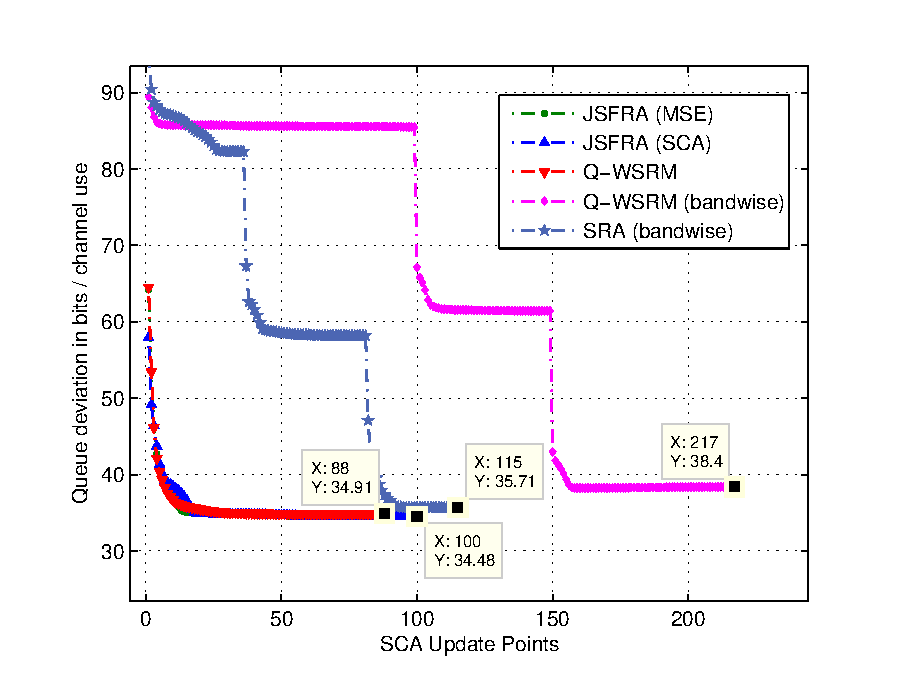
\includegraphics[width=1.0\textwidth]{fig-1-1}
\caption{\me{4 \times 1} system}
\label{fig-1}
\end{subfigure}
\hfill
\begin{subfigure}{0.49\textwidth}
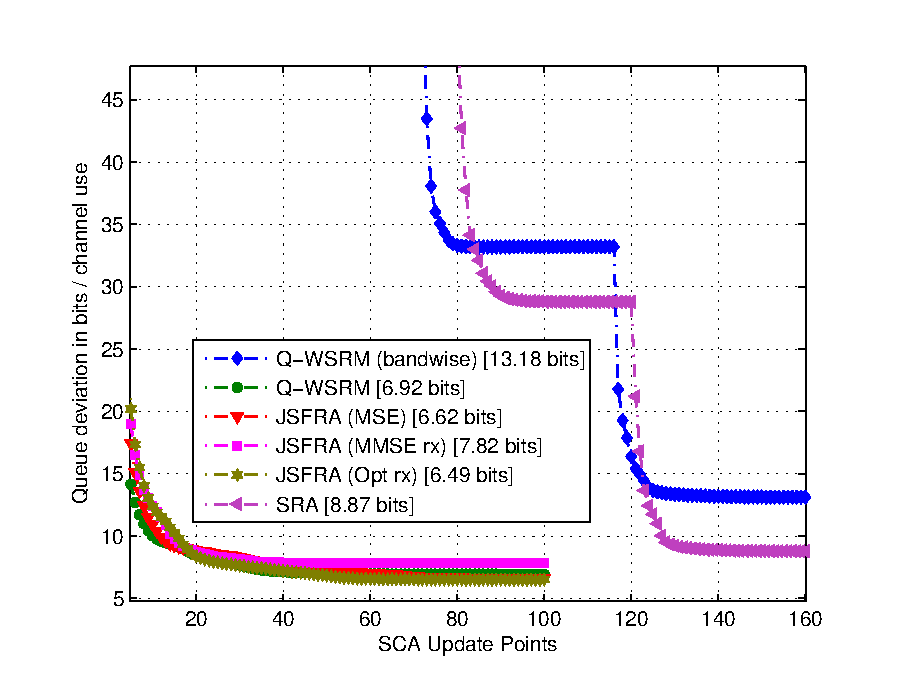
\includegraphics[width=1.0\textwidth]{fig-2-1}
\caption{\me{4 \times 2} system}
\label{fig-2}
\end{subfigure}
\caption{Convergence plot for \me{\lbrace N,N_B,K \rbrace = \lbrace 3,3,9 \rbrace} model}
\end{figure*}

In the sub-channel wise allocations, where the total transmit power is shared equally among the sub-channels, the precoders are designed for each sub-channels independently. In this approach, the precoders are coupled via the number of queued bits which are updated using \eqref{eqn-weight} before designing the precoders for the sub-channels. At each \ac{SCA} points, the number of queued bits are reduced significantly with the introduction of a new sub-channel since the algorithm starts with a random inital point before it converges to an optimal\footnote{due to the nonconvex nature of the original problem} precoders. The total number of backlogged bits at each \ac{SCA} update instant are plotted in Fig. \ref{fig-1} for the discussed centralized schemes and the convergence point are marked with the data tips. Fig. \ref{fig-2} compares the performance of the centralized algorithms for the \me{N_R = 2} receive antennas.
\begin{table}
\centering
\renewcommand{\arraystretch}{1.25} \scriptsize
\begin{tabular}{|c|*{8}{c}|c|}
\hline
\me{q} & \multicolumn{8}{c|}{user indices} & \me{\chi} \\
\hline
\me{1} & 15.00 & 3.95 & 5.26 & 8.95 & 7.03 & 11.90 & 12.00 & 9.73 & 25.15 \\
\me{2} & 11.23 & 3.93 & 10.76 & 10.65 & 10.27 & 9.68 & 8.77 & 5.90 & 27.77 \\
\me{\infty} & 11.41 & 4.41 & 10.41 & 10.41 & 10.41 & 8.41 &  8.41 &  6.41 & 28.68 \\
\hline
\me{Q_k}  & 15.0 &  8.0 &  14.0 & 14.0 &  14.0 & 12.0 & 12.0 & 10.0  \\    
\cline{1-9}
\end{tabular}
\caption{Queue information for the system \me{\lbrace N,N_B,K,N_R \rbrace = \lbrace 5,2,8,1 \rbrace}}
\label{tbl-3}
\end{table}

The behavior of the \ac{JSFRA} algorithm for different exponents \me{q} are outlined in the Table \ref{tbl-3} for the users located at the cell-edge of the system employing \me{N_T = 4} transmit antennas. The configuration is mentioned in the caption of Table \ref{tbl-3} along with the number of queued bits for each user. It is evident that the algorithm minimizes the queued bits for the \me{\ell_1} norm compared to the \me{\ell_2} norm, which is shown in the column displaying the total number of left over packets \me{\chi} in bits. The \me{\ell_{\infty}} norm provides fair allocation of the resources by making the left over packets \me{\chi_k = 3.58} bits. The \me{\ell_{\infty}} norm provides the fair allocation by making the queued deviation equal for all the users after the current allocation irrespective of their channel gains.


\subsection{Distributed Solutions}
The distributed algorithms are compared using the total number of backlogged packets after each \ac{SCA} update. Fig. \ref{fig-d} compares the performances of the algorithms with the \ac{PL} varies uniformly between \me{[0,-6]} dB and each \ac{BS} serves \me{|\mc{U}_b| = 4} users. As discussed in Section \ref{sec-4}, the performance and the convergence speed of the distributed algorithms are susceptible to the step size \eqn{\rho^{(i)}}. Due to the fixed interference levels in the primal approach, it may lead to infeasible solutions if the initial or any intermediate update is not feasible.

Fig. \ref{fig-d} compares the performance of the \ac{JSFRA} schemes discussed in Sections \ref{sec-3.2.1} and \ref{sec-3.3} using primal and \ac{ADMM} approaches. For each \ac{SCA} update, the primal or the \ac{ADMM} scheme is performed for \me{J_{\max} = 20} iterations to exchange the respective coupling variables. The number of backlogged packets only at the \ac{SCA} points are marked in the figure. The performance of the distributed approaches is similar to that of the centralized schemes if the distributed algorithms are allowed converge. However, in our simulations, we observe that \eqn{J_{\max} = 20} is sufficient for the \ac{ADMM} to converge. 

%In Fig. \ref{fig-d}, the total number of backlogged packets at each \ac{SCA} points are plotted without the inner loop iterations of \me{J_{\max}} times for the primal or the dual variables convergence. %It can be seen from Fig. \ref{fig-d} that the distributed algorithms approach the centralized scheme by exchanging minimal information between the coordinating \acp{BS}.

Fig. \ref{fig-d-3.1} compares the performances of the centralized and the \ac{KKT} algorithm in Section \ref{sec-4.3} for different exponents with \ac{PL} chosen uniformly between \me{[0,-3]} dB. The \me{\ell_1} norm \ac{JSFRA} scheme performs better over other schemes due to the greedy nature of the objective. The \ac{KKT} approach for \me{\ell_1} norm is not defined due to the non-differentiability of the objective as discussed in Section \ref{sec-4.3}. If used for \me{\ell_1} norm, the over-allocation will not affect the dual variables \me{\sigma_{l,k,n}} and \me{\alpha_{l,k,n}} since the queue deviation is raised to the power zero in \eqref{kkt-mse-4.2}. A heuristic method is proposed in Fig. \ref{fig-d-3.1} by assigning zero for \me{\sigma_{l,k,n}} when \me{Q_k - t_k < 0} to addresses the over-allocation. The heuristic approach oscillates near the converging point with the deviation determined by the factor \me{\rho} used in \eqref{kkt-mse-4.1}. The objective values are mentioned in the legend for all the schemes and the \me{\ell_1} norm is used for comparison.
\begin{figure}
	\centering
	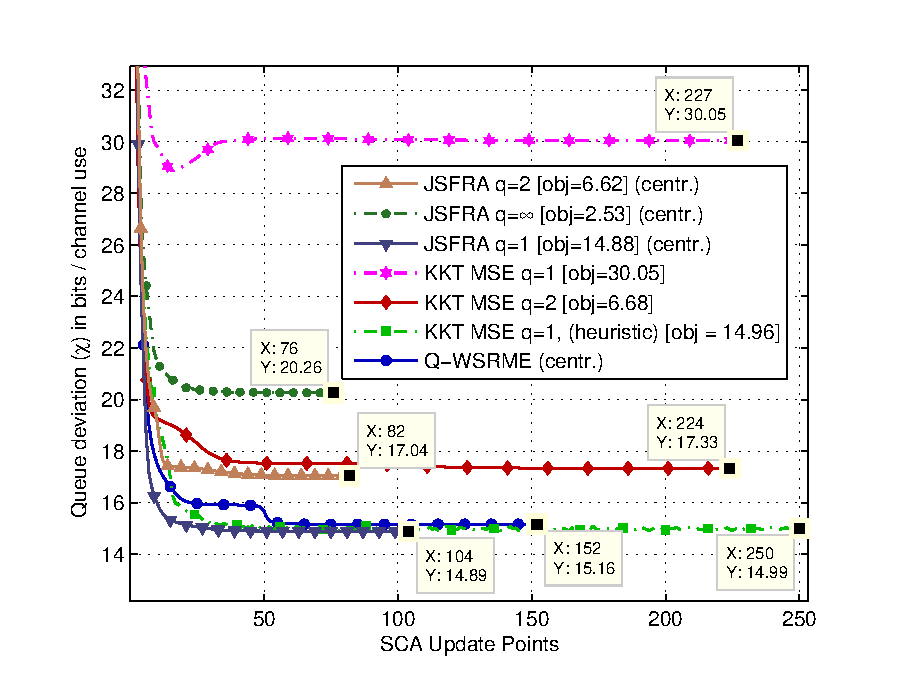
\includegraphics[width=\columnwidth]{fig-9-3}
	\vspace{-0.2in}
	\caption{Impact of varying \me{q} on the total number of backlogged packets after each \ac{SCA} update for a system \me{\lbrace N,N_B,K,N_T,N_R \rbrace = \lbrace 5,2,8,4,1 \rbrace} and \me{Q_k = [9,16,14,16,9,13,11,12]} bits}
	\label{fig-d-3.1}
\end{figure}

\begin{comment}
The \me{\ell_2} norm for the \ac{JSFRA} and the \ac{KKT} approach achieves nearly the same value of \me{6.62} with different \me{\chi}, due to the limited number of iterations for the dual variable convergence between each \ac{SCA} update. Fig. \ref{fig-d-3.1} also shows the effect of dropping the squared rate variable from the objective in the \ac{Q-WSRME} scheme compared to the \me{\ell_2} norm which includes it. By dropping it, the \ac{Q-WSRME} scheme minimizes the number of queued packets in a prioritized manner based on the respective queues. On contrary, the \me{\ell_2} norm allocate rates to the users with the higher number of queued packets before addressing the users with the smaller number of queued packets.

In Fig. \ref{fig-d-2}, the performance of the distributed algorithms are studied for \me{K = 12} users utilizing \me{N = 6} sub-channels. The system considers \me{N_B = 3} \acp{BS}, each having \me{N_T = 4} transmit antennas serving \me{|\mc{U}_b| = 4} users equipped with \me{N_R = 2} antennas respectively. The users are assumed to have the path loss following the uniform distribution between \me{[0,-6]} dB from all \acp{BS}. The performance of the algorithms are similar to the \me{N_B = 2} \ac{BS} scenario discussed earlier.

Fig. \ref{fig-d-2} plots the performance of the centralized and the distributed algorithms at each \ac{SCA} update. In case of the distributed approaches, in between each \ac{SCA} update, the primal or the \ac{ADMM} exchanges are performed for \me{J_{\max} = 20} iterations. In practice, \me{J_{\max} = 1} can be set to perform the \ac{SCA} update, \ac{ADMM} or primal update, and the receive beamformers \me{\mvec{W}{k,n}} update at the same instant, which affects the convergence rate and the stationary point of the final solution. The data tips are used to highlight the convergent points of various algorithms. The performance of the \ac{JSFRA} schemes using the primal decomposition are notably inferior compared to the \ac{ADMM} approach for the same schemes. It is mainly attributed to the difficulty in selecting the step size for the system employing \me{N_B \geq 3} \acp{BS}.
\begin{figure*}[t]
	\centering
	\subfloat[][System \me{\lbrace N,N_B,K,N_R \rbrace = \lbrace 3,2,8,1 \rbrace}]{
		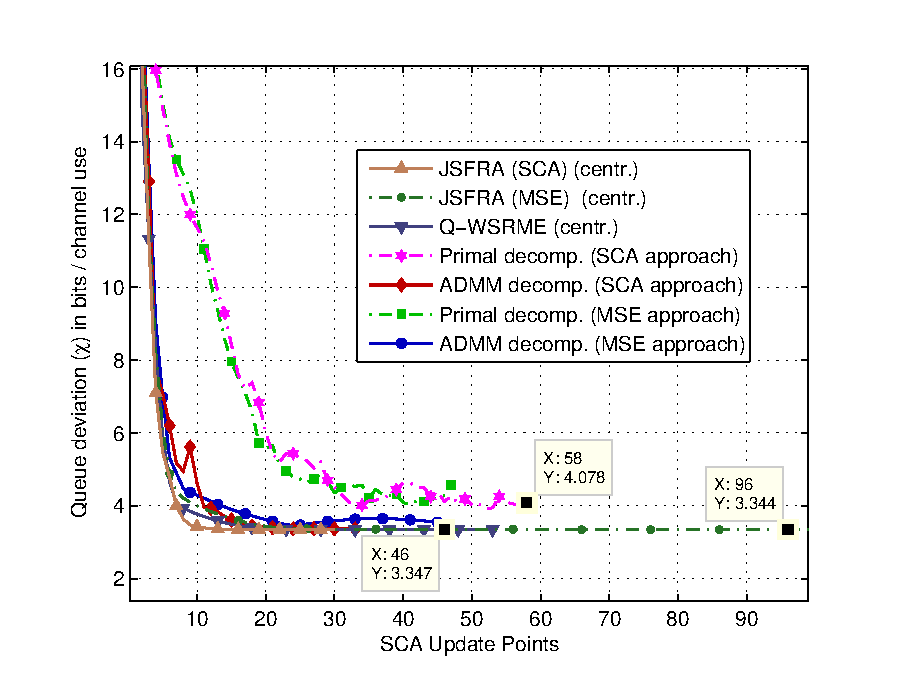
\includegraphics[width=0.48\textwidth]{fig-3-2}
		\label{fig-d-1}
	}
	\hfill
	\subfloat[][System \me{\lbrace N,N_B,K,N_R \rbrace = \lbrace 6,3,12,2 \rbrace}]{
		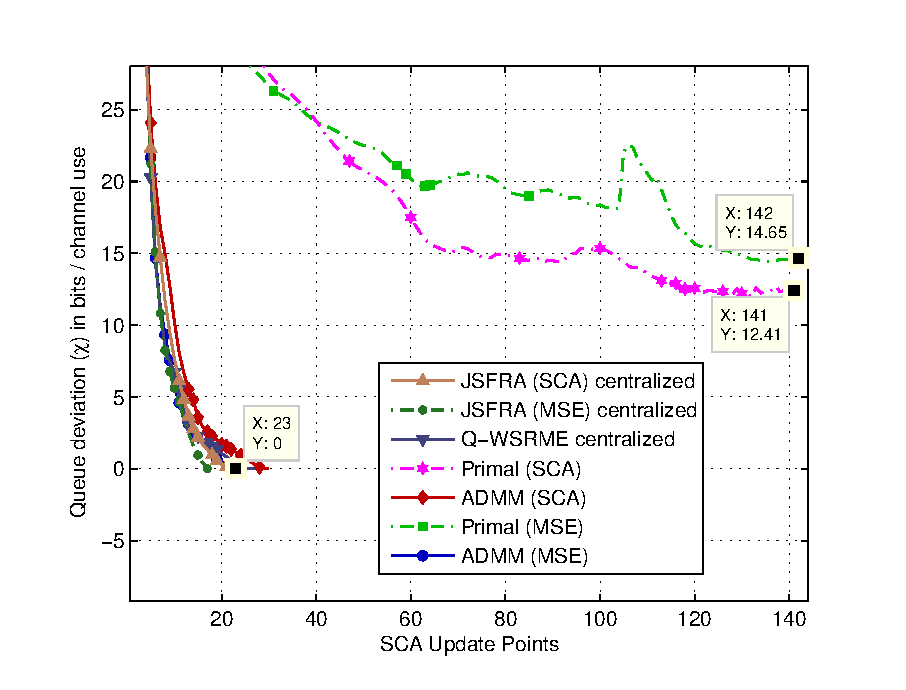
\includegraphics[width=0.48\textwidth]{fig-5-1}
		\label{fig-d-2}
	}
	\caption{Number of backlogged packets at each \ac{SCA} points}
	\label{fig-d}
\end{figure*}

\end{comment}

\subsection{Average Backlogged Packets Over Slots}

\review{
We discuss the performance of the \ac{JSFRA} algorithm for different \me{\ell_q} over multiple transmission slots. It is compared to the existing \ac{Q-WSRME} scheme by varying the average arrival rate \me{A_k} of all users. Fig. \ref{fig-time-analysis} plots the performances of the centralized algorithms for different \me{\ell_q} values. Even though \me{A_k}'s are constant for all users, the instantaneous arrivals are random and they follow the Poisson process. We considered a \me{4 \times 1} \ac{MIMO} with \me{N = 4} sub-channels and \me{N_B = 2} \acp{BS}. The \ac{PL} is modeled as a uniform random variable \me{[0,-3]} dB.

Fig. \subref*{fig-review} compares various schemes with the average number of backlogged packets present in the system after each transmission slot. The performance of the \ac{JSFRA} scheme using \me{\ell_2} is similar to the \ac{Q-WSRME} approach in the average number of residual packets after each transmission slot. Note that the additional rate constraints in the \ac{Q-WSRME} scheme is the reason for the equivalence. Both \ac{Q-WSRM} and \ac{Q-WSRME} performs similar to \me{\ell_2} \ac{JSFRA} scheme when the arrival rates are larger than those of the actual transmissions. Fig. \ref{fig-time-analysis} shows that the number of backlogged packets are noticeably less for the \me{\ell_1} \ac{JSFRA} scheme due to the greedy allocation of serving users with better channel. Fig. \ref{fig-time-analysis} highlights that the \me{\ell_{\infty}} \ac{JSFRA} scheme performs equally well compared to the other objectives when the system is in the stable region. On contrary, the performance is inferior in the unstable region, since the fair allocation is not effective when the number of backlogged packets is large for all users.
}

%acresetall
\section{Conclusions} \label{sec-6}

In this work, we presented the \acl{QM} objective to minimize the number of backlogged packets by designing the transmit precoders across the space-frequency dimension in a multi-cell \ac{MU} \ac{MIMO} system. We proposed the \ac{JSFRA} scheme, which adopts the \ac{SCA} technique to model the nonconvex constraint as a convex constraint in an iterative manner to design the precoders for the \acl{QM} objective. We also proposed an alternative approach using the \ac{MSE} relaxation for the same problem when the receive beamformers are based on the \ac{MMSE} receivers. The exponent used in the proposed formulation can be modified to achieve either greedy allocation or equally fair allocation. We also proposed the distributed solutions for the proposed centralized \ac{JSFRA} problem using the \ac{ADMM} method, which has better convergence behavior compared to the primal decomposition. In addition, we also proposed an iterative algorithm based on the \ac{KKT} conditions for the \ac{MSE} reformulated \ac{JSFRA} scheme to design the precoders in a distributed manner using the closed form solutions.

\appendices

%\section{\acl{PD} approach} \label{a-2}
%By fixing the interference values \me{\zeta_{\pr{l},\pr{k},n,{b_k}}} corresponding to the interference from the \ac{BS} \me{b_k}, the constraint involving the coupling variables \eqref{eqn-9.1c} can be relaxed using the equivalent formulation in \eqref{eqn-decent-3}. Now, the subproblem for the \ac{BS} \me{b_k \in \mc{B}} can be obtained by grouping the terms relevant to the \ac{BS} \me{b_k} as
\begin{IEEEeqnarray}{rCl} \label{eqn-primal-1}
\underset{\substack{\gamma_{l,k,n} \\ \mvec{m}{l,k,n}, \beta_{l,k,n}}}{\text{minimize}} &\quad & \| \tilde{\mbf{v}}_{b_k} \|_q \IEEEyessubnumber \label{eqn-primal-1a} \\
\text{subject to}&\quad&\sum_{n = 1}^N \sum_{k \in \mathcal{U}_{b_k}} \text{tr} \, (\mvec{M}{k,n} \mvec{M}{k,n}^\herm) \leq P_{{\max}}, \IEEEyessubnumber \label{eqn-primal-1c} \\
&& \beta_{l,k,n} \geq \sum_{\substack{j = 1\\j \neq l}}^L |\mvec{w}{l,k,n}^\herm \mvec{H}{{b_k},k,n} \mvec{m}{j,k,n} |^2 \nonumber \\
&&\quad + \sum_{i \in \mc{U}_{b_k} \backslash \{k\}} \sum_{j = 1}^L |\mvec{w}{l,k,n}^\herm \mvec{H}{{b_k},k,n} \mvec{m}{j,i,n} |^2 + \sum_{b \in \bar{\mc{B}}_{b_k}} \zeta_{l,k,n,b} \; + \; N_0\|\mvec{w}{l,k,n}\|^2 \IEEEyessubnumber \label{eqn-primal-1d} \\
&& \zeta_{\pr{l},\pr{k},n,{b_k}} \geq \sum_{k \in \mc{U}_b} \sum_{l = 1}^L |\mvec{w}{\pr{l},\pr{k},n}^\herm \mvec{H}{b_k,\pr{k},n} \mvec{m}{l,k,n} |^2, \; \forall \pr{k} \in \bar{\mc{U}}_{b_k}, \; \forall n \in \mc{C} \IEEEyessubnumber \label{eqn-primal-1e} \\
 & \quad & \text{and} \; \eqref{eqn-8} \IEEEyessubnumber,
\end{IEEEeqnarray}

Let \me{\mbfa{\zeta}^{\set{b_k}}} be the vector representing the fixed interference levels relevant to the \ac{BS} \me{b_k} in a fully connected network\footnote{in practice it will be less due to the path loss}, which is given by
\begin{IEEEeqnarray}{RCL} \label{eqn-primal-2}
\mbfa{\zeta}_{k,n,b} &=& \left [ \; \zeta_{1,k,n,b}, \dotsc, \zeta_{L,k,n,b} \; \right ] \IEEEyessubnumber \\
\mbfa{\zeta}^{\set{b_k}}_n &=& \left [ \; \mbfa{\zeta}_{\mc{U}_{b_k}(1),n,\bar{\mc{B}}_{b_k}(1)}, \dotsc, \mbfa{\zeta}_{\mc{U}_{b_k}(1),n,\bar{\mc{B}}_{b_k}(|\bar{\mc{B}}_{b_k}|)}, \right . \nonumber \\
&& \left . \dotsc, \mbfa{\zeta}_{\mc{U}_{b_k}(|\mc{U}_{b_k}|),n,\bar{\mc{B}}_{b_k}(|\bar{\mc{B}}_{b_k}|)}, \dotsc, \mbfa{\zeta}_{\bar{\mc{U}}_{b_k}(1),n,b_k}, \dotsc, \mbfa{\zeta}_{\bar{\mc{U}}_{b_k}(|\bar{\mc{U}}_{b_k}|),n,b_k} \; \right  ] \IEEEyessubnumber \\
\mbfa{\zeta}^{\set{b_k}} &=& \left [ \; \mbfa{\zeta}^{(b_k)}_1, \dotsc, \mbfa{\zeta}^{(b_k)}_N \; \right ], \IEEEyessubnumber
\end{IEEEeqnarray}
where the length of the vector \me{\mbfa{\zeta}^{\set{b_k}}} is
\begin{equation}
n_{b_k} = | \mbfa{\zeta}^{\set{b_k}} | = \left ( |\bar{\mc{B}}_{b_k}| |\mc{U}_{b_k}| + |\bar{\mc{U}}_{b_k}|\right ) L N
\label{primal-vec-len}
\end{equation}

The local subproblem \eqref{eqn-primal-1} solved at each \ac{BS} are coordinated by the master problem, which updates the interference thresholds \me{\mbfa{\zeta}^{\set{b}}, \forall b \in \mc{B}} for the next iteration. The master problem controlling multiple subproblems is given by
\begin{IEEEeqnarray}{rCl} \label{eqn-primal-3}
\underset{\mbfa{\zeta}}{\text{minimize}} & \quad & \sum_{b \in \mc{B}} \alpha^{\star}_b (\mbfa{\zeta}^{\set{b}}) \IEEEyessubnumber \\
\text{subject to} & \quad & \mbfa{\zeta}^{\set{b}} \in \mathbb{R}_+^{n_b}, \forall b \in \mc{B}, \IEEEyessubnumber
\end{IEEEeqnarray}
where \me{\alpha^{\star}_b (\mbfa{\zeta}^{\set{b}})} denotes the optimal solution for \eqref{eqn-primal-1} with the previous value of \me{\mbfa{\zeta}^{(i-1)}}, where \me{\mbfa{\zeta}} is the global interference vector formed by stacking the interference vector associated with each \ac{BS} as \me{\mbfa{\zeta} = \left [ \mbfa{\zeta}^{\set{\mc{B}(0)}}, \mbfa{\zeta}^{\set{\mc{B}(1)}}, \ldots, \mbfa{\zeta}^{\set{\mc{B}(|\mc{B}|)}}\right ]}.

The master problem to find the optimal \me{\mbfa{\zeta}^{\set{b_k}(i)}, \forall b_k \in \mc{B}} is given by the following subgradient method \cite{bertsekas1999nonlinear} as
\begin{equation} \label{primal-sg-update}
\zeta^{\set{b_k}(i)}_{l,k,n,b} = \left [\zeta_{l,k,n,b}^{\set{b_k}(i-1)} - \rho \, s_{l,k,n,b}^{\set{b_k}(i-1)} \right ]^+, \forall b \in \mc{B}, \forall k \in \bar{\mc{U}}_b,
\end{equation}
where \me{i} is the iteration index, \me{\rho} is the positive step size, and \me{s^{\set{b_k}(i-1)}_{l,k,n,b}} is the subgradient of the problem defined in \eqref{eqn-primal-3} evaluated at \me{\zeta^{(i-1)}_{l,k,n,b}}. To find the subgradient \me{s^{\set{b_k}(i-1)}_{l,k,n,b}}, the dual variables corresponding to the interference constraints are required, which can be obtained by forming the dual problem of \eqref{eqn-primal-2} as discussed in \cite{pennanen2011decentralized}. Now the primal and the dual variables \me{\mu^{\set{b_k}}_{l,k,n}} and \me{\mu^{\set{b_k}}_{\pr{l},\pr{k},n}} corresponding to the constraints \eqref{eqn-primal-1d} and \eqref{eqn-primal-1e} can be obtained from the solvers, which solves the dual problem as well.

To obtain the next interference iterate at each \ac{BS}, the locally evaluated dual variables are exchanged among the \acp{BS} in the set \me{\mc{B}} in order to obtain the next interference vector in a distributed manner. Once we obtain the dual variables from all the \acp{BS}, the subgradients relevant to the \ac{BS} \me{b_k} are evaluated by taking the difference between the two \acp{BS} associated with each interference value, \textit{i.e}, \me{s^{\set{b_k}(i)}_{l,k,n,b} = \mu^{\set{b_k}}_{l,k,n} - \mu^{\set{b}}_{l,k,n}}. With the newly estimated subgradient value \me{s^{\set{b_k}(i)}_{l,k,n,b}}, the interference terms corresponding to the \ac{BS} \me{b_k} are updated using \eqref{primal-sg-update}. The algorithmic representation of the \ac{PD} approach is detailed in Algorithm. \ref{algo-2}.
\begin{algorithm}
 \SetAlgoLined
 \DontPrintSemicolon
 \BlankLine
 \SetKwInput{KwInit}{Initialize}
 \KwIn{\me{a_k, \, Q_k, \, \mvec{H}{b,k,n},\; \fall b \in \mathcal{B}, \, \fall k \in \mathcal{U}, \fall n \in \mathcal{C}}}
 \KwOut{\me{\mvec{m}{l,k,n}} and \me{\mvec{w}{l,k,n} \fall l \in \set{1,2,\dotsc,L}}}
 \KwInit{\me{i=0} and the transmit precoders \me{\tilde{\mbf{m}}_{l,k,n}} randomly satisfying the total power constraint \eqref{eqn-4.3}}
 update \me{\mvec{w}{l,k,n}} with \eqref{eqn-10} and \me{\tilde{\mbf{u}}_{l,k,n}} with \eqref{eqn-8} using \me{\tilde{\mbf{m}}_{l,k,n}} \;
 initialize the interference threshold \me{\zeta_{l,k,n,b}^{\set{0}} \forall b \in \mc{B}, \forall k \in \bar{\mc{U}}_{b_k}, \forall l,n} \;
 for each \ac{BS} \me{b \in \mc{B}}, perform the following procedure \;
 \Repeat{convergence or \me{i \geq I_{\max}}}{
    initialize \me{j=0} \;
    \Repeat{convergence or \me{j \geq J_{\max}}}{
        solve for the transmit precoders \me{\mvec{m}{l,k,n}} and dual variables \me{\mu^{\set{b}}_{l,k,n}} using \eqref{eqn-primal-2} \;
        exchange \me{\mu^{\set{b}}_{l,k,n}} across the coordinating \acp{BS} in \me{\mc{B}} \;
        update \me{\zeta^{\set{b}(j+1)}_{l,k,n,b}} using \eqref{primal-sg-update} locally \;
        \me{j = j + 1} \;
    }
    update the receive beamformers \me{\mvec{w}{l,k,n}} using \eqref{eqn-10} with the recent precoders \me{\mvec{m}{l,k,n}} \;
    exchange the receive precoders \me{\mbf{W}_{k,n}} \me{\forall k \in \mc{U}_b} among the \acp{BS} in \me{\mc{B}} \;
    update \me{\tilde{p}_{l,k,n}}, \me{\tilde{q}_{l,k,n}} and \me{\tilde{\beta}_{l,k,n}} with the recent precoders using \eqref{eqn-wsrm-expr} and \eqref{eqn-6.3} for the \ac{SCA} approach (or) \;
    update \me{\tilde{\epsilon}_{l,k,n}} with the recent precoders using \eqref{eqn-mse-2.3} with equality for the \ac{MSE} formulation approach \;
    $i = i + 1$ \;
  }
 \caption{Decentralization via Primal Decomposition for \acs{JSFRA} scheme}
  \label{algo-2}
\end{algorithm}


\section{Tightness of \ac{SINR} relaxation} \label{a-3}
\review{\begin{comment}
For the constraints \eqref{eqn-6.2} and \eqref{eqn-6.3} to be active, there should be at least one user in each \ac{BS} with enough backlogged packets that cannot be served with the given power budget. To prove this, let us consider a \ac{BS} \me{b} with \me{N_T \times 1} system serving \me{|U|_b} users each with \me{Q_k} backlogged packets. The \ac{JSFRA} formulation can be written as
\begin{IEEEeqnarray}{rCl} \label{tight}
	\underset{\gamma_{k},\mvec{m}{k},\beta_{k}}{\text{minimize}} &\quad& \sum_{k \in \mc{U}_b} \big | Q_k - \log_2(1 + \gamma_k) \big |^q  \eqsub \\
	\text{subject to} &\quad& \gamma_{k} \leq \frac{ | \mvec{H}{k} \mvec{m}{k}|^2}{\beta_{k}} \IEEEyessubnumber \label{ae-1} \\
	&\quad& \beta_{k} \geq N_0 + \sum_{\mathclap{i \neq k}} |\mvec{H}{k} \mvec{m}{i} |^2 \IEEEyessubnumber \label{ae-2} \\
	&\quad& \sum_{k \in \mc{U}_b} \trace \, (\mvec{m}{k} \mvec{m}{k}^\herm) \leq P_{{\max}}. \IEEEyessubnumber \label{ae-3}
\end{IEEEeqnarray}
Let \me{N_T > |\mc{U}_b|} and the precoders are found by solving \eqref{tight} with a nonzero objective value at the optimal point. Let us consider two users, say \me{i} and \me{j} with precoders \me{\mvec{m}{i}} and \me{\mvec{m}{j}}. In order to show the tightness of \eqref{ae-1} and \eqref{ae-2}, let us assume by contradiction that \eqref{ae-1} and \eqref{ae-2} are not tight for user \me{i} only. Let us also consider that \me{\gamma_k} for all users \me{k \in \mc{U}_b \backslash j} are identified to satisfy the backlogged packets. 

Now, in order to minimize the objective of the \me{\ith{i}} user, \me{\gamma_i} should be \me{2^{Q_i} - 1} to have the minimum objective. Since the constraints \eqref{ae-1} and \eqref{ae-2} are not tight for the \me{\ith{i}} user, the actual \ac{SINR} on the r.h.s of \eqref{ae-1} is greater than \me{\gamma_i}. It is attributed to the excess power in the transmit precoder of user \me{i} as \me{\mvec{m}{i} = \bar{\mbf{m}}_{i} + \mbf{V}_i \mbf{e}}, where \me{\mvec{V}{i} = \mc{N}([\mbf{H}^{\mathrm{T}}_0, \dotsc, \mbf{H}^{\mathrm{T}}_{i-1},\mbf{H}^{\mathrm{T}}_{i+1}, \dotsc,\mbf{H}^{\mathrm{T}}_{|\mc{U}_b| - 1}]^{\mathrm{T}})} denotes the null space corresponding to the other user channel vectors and \me{\mbf{e}} be any random vector with power \me{\Delta P}. Note that the extra power has no impact on the interference constraint \eqref{ae-2} of other users. 

Since the allocated rate of user \me{j} is less than the queued packets, we can find a precoder \me{\mvec{m}{j}} with the additional power of \me{\Delta P} as \me{\mvec{m}{j}^\prime = \bar{\mbf{m}}_{j} + \mvec{V}{j} \mbf{e}^\prime}. Note that the new precoder has no impact on the interference constraint of other users. The newly found precoder \me{\mvec{m}{j}^\prime} minimize the queue of user \me{j} without affecting the rates of other user, there by reduces the objective further. It is in contradiction to our original assumption that the precoders are optimal and the objective is minimum. 

It can be seen that the constraints are tight as long as there is one user with unserviced backlogged packets at each \ac{BS} with the given power budget. Since the objective is not to minimize power, when the power budget is more than sufficient to service the backlogged packets of all users, the \ac{JSFRA} scheme is not guaranteed to find the minimum power precoders to empty the current backlogged packets in the system. The objective of the \ac{JSFRA} problem can be regularized by including the power term to find the minimum power precoders as
\begin{equation*}
\| \tilde{\mbf{v}} \|_q + \varphi \sum_{k \in \mc{U}} \sum_{n = 1}^{N} \sum_{l=1}^{L} \mathrm{tr} \left ( \mvec{m}{l,k,n} \mbf{m}^\herm_{l,k,n} \right ),
\end{equation*}
for a small \me{\varphi} without affecting the optimal solution. Note that the above objective is guaranteed to make the constraints \eqref{eqn-6.2} and \eqref{eqn-6.3} active by relaxing the power constraint \eqref{eqn-6.4}.
\end{comment}

For the constraints \eqref{eqn-6.2} and \eqref{eqn-6.3} to be active, there should be at least one user in each \ac{BS} with enough backlogged packets that cannot be served with the given power budget. On the other hand, to make the constraints active in all cases, the objective of the \ac{JSFRA} formulation should be regularized with the transmit power without affecting the solution as
\begin{equation*}
\| \tilde{\mbf{v}} \|_q + \varphi \sum_{k \in \mc{U}} \sum_{n = 1}^{N} \sum_{l=1}^{L} \mathrm{tr} \left ( \mvec{m}{l,k,n} \mbf{m}^\herm_{l,k,n} \right )
\end{equation*}
where \me{\varphi \approx 0}. Note that the modified objective will relax the power constraint by making the constraints \eqref{eqn-6.2} and \eqref{eqn-6.3} active at the final solution.

}

\section{Convergence Analysis of Centralized Algorithm} \label{sec-3.5}
\review{\newcommand{\eqn}[1]{\(#1\)}
\newcommand{\mx}{\mbf{x}}
\newcommand{\my}{\mbf{y}}
\newcommand{\mz}{\mbf{z}}
\newcommand{\mxb}{{{\mbf{x}}}}
\newcommand{\myb}{{{\mbf{y}}}}
\newcommand{\iterate}[2]{{#1}^{(#2)}}
\newcommand{\iter}[3]{{#1}_{#2}^{(#3)}}

\subsubsection{Centralized Problem}

Let us express the \ac{JSFRA} problem in \eqref{eqn-6} and \eqref{eqn-mse-1} as
\begin{IEEEeqnarray}{rCl} \label{con}
\underset{\mx,\my,\mz}{\text{minimize}} &\quad& f(\mz) \eqsub \label{con-obj} \\
\text{subject to} &\quad& h(\mz) - g_0(\mx,\my) \leq 0 \eqsub \label{con-dc} \\
&\quad& g_1(\mx,\my) \leq 0, \eqsub \label{con-cvx-blk} \\
&\quad& g_2(\mx) \leq 0, \eqsub \label{con-cvx}
\end{IEEEeqnarray}
wher \me{g_2,f} are convex functions and \me{h} is a linear function. Let \me{g_0,g_1} are convex functions only on \me{\mx} or \me{\my} as the variable but not on both. Note that the \eqref{con-dc} correspond to the constraints in \eqref{eqn-6.2} and \eqref{eqn-mse-1.2} and \eqref{con-cvx-blk} corresponds to the constraints in \eqref{eqn-6.3} and \eqref{eqn-mse-1.3}. Other convex constraints are addressed by the constraint \eqref{con-cvx}. With this, the feasible set of the problem \eqref{con} is given by 
\begin{IEEEeqnarray}{rl}
\mc{F} &= \{ \mx,\my,\mz | h(\mz) - g_0(\mx,\my) \leq 0, g_1(\mx,\my) \leq 0, g_2(\mx) \leq 0\} \nonumber
\end{IEEEeqnarray}

In order to solve the problem, we resort to \ac{AO} by fixing a block of varibles and optimize for others. In the problem \eqref{con}, even after fixing the variable \me{\my}, the problem is nonconvex due to the \ac{DC} constraint in \eqref{con-dc}. In order to solve the problem after fixing the variable \me{\my}, we adopt the \ac{SCA} approach presented in \cite{lipp2014variations,lanckriet2009convergence,scutari_1} by relaxing the nonconvex set by a sequence of convex subsets. Since the proposed method involves two level of iterations, we denote the \ac{AO} iteration index by a superscript \me{(i)} and the \ac{DC} constraint relaxations by a subscript \me{k}. Let \me{\iter{\mc{X}}{k}{i}} be a feasible set for the \eqn{\ith{i}} \ac{AO} iteration and the \me{\ith{k}} \ac{SCA} point for a fixed \me{\my} and for a fixed \me{\mx}, the set is represented as \me{\iter{\mc{Y}}{k}{i}}. Since the \ac{SCA} iterations are performed until convergence, let \me{\iter{\mx}{\ast}{i}} denotes the converged point of \me{\mx} in the \me{\ith{i}} \ac{AO} iteration.

Without affecting the convergence proof, let us consider the variable \me{\my} is fixed in the iteration \me{i} for \ac{AO} and \me{k} for the \ac{SCA} problem to solve for the unique minimizer for \me{\mx \in \iter{\mc{X}}{k}{i}}. 


In order to solve for a suboptimal solution, let us resort to the \ac{AO} by fixing a block of variables and optimize for others. Before proceeding further, let us define the following notations. Let \me{\iter{\mx}{k}{i}} denote the \me{\ith{i}} \ac{AO} operating point and \me{k} represent the \me{\ith{k}} \ac{SCA} point. Let us define a set \eqn{\iter{\mc{X}}{k}{i}} as set of feasible values of the subproblem in the \me{\ith{i}} \ac{AO} iteration and the \me{\ith{k}} \ac{SCA} optimization point for a fixed variable \me{\my}. Since \ac{AO} is an iterative method, let us begin by fixing \me{\my} with the previously found optimal value \me{\iter{\myb}{\ast}{i-1} \in \iter{\mc{Y}}{\ast}{i-1} \subset \mc{F}}, where \me{\ast} in subscript denotes the optimal value over some set \me{\mc{Y}}. Now the problem in \eqref{con} is still nonconvex due to the constraint \eqref{con-dc}, which is in \ac{DC} form. Following the approaches presented in \cite{lipp2014variations,lanckriet2009convergence,scutari_1}, the function \me{g_0(\mx,\iter{\myb}{\ast}{i-1})} is linearized around a fixed feasible point \me{\iter{\mxb}{\ast}{i} \in \iter{\mc{X}}{\ast}{i-1} \subset \mc{F}} by
\begin{equation} \label{con-relax}
\hat{g}_o(\mx,\iter{\myb}{\ast}{i-1});\iter{\mx}{k}{i})) = {g}_0(\iterate{\mxb}{0},\iterate{\myb}{0}) + \nabla g_0(\iterate{\mxb}{0},\iterate{\myb}{0})^\mathrm{T} (\mx - \iterate{\mxb}{0}).
\end{equation}
Using the relaxation \eqref{con-relax}, the convex subproblem for the \me{\ith{i}} \ac{AO} iterate of \me{\myb} and the \me{\ith{k}} linear approximation of \me{\mxb} as
\begin{subeqnarray} \label{con-m}
	\underset{\mx,\my,\mz}{\text{minimize}} &\quad& f(\mz) \eqsub \label{con-obj-m} \\
	\text{subject to} &\quad& h(\mz) - \hat{g}_0(\mx,\iterate{\myb}{i};\iterate{\mxb}{k}) \leq 0 \eqsub \label{con-dc-m} \\
	&\quad& g_1(\mx,\iterate{\myb}{i}) \leq 0, \eqsub \label{con-cvx-blk-m} \\
	&\quad& g_2(\mx) \leq 0, \eqsub \label{con-cvx-m}
\end{subeqnarray}
Let the set defined by the problem in \eqref{con-relax} be represented as \me{\iterate{\mc{X}}{i}_{k} \subset \mc{F}}, where \me{\mc{X}} denotes the subset in which \me{\my} is fixed. In order to prove the convergence of the convex subproblem \eqref{con-m} for a fixed \me{\iterate{\myb}{i}} and \me{\iter{\mxb}{k}{i}}, let us assume that \eqref{con-m} yields \me{\mx_{k+1}} and \me{\mz_{k+1}} as the solution at the \me{\ith{k}} iteration. To show that \me{\mx_{k+1}} and \me{\mz_{k+1}} minimizes the objective function ans also feasible, let us assume that the point \me{\iterate{\mxb}{k}} is feasible for \eqref{con-m}. Since the function \me{{g}_0(\mx,\iterate{\myb}{i})} is linearized around \me{\iterate{\mxb}{k}}, it satisfies
\begin{equation}
h(\mz) - {g}_0(\mx,\iterate{\myb}{i}) \leq h(\mz) - \hat{g}_0(\mx,\iterate{\myb}{i};\mxb_k) \leq 0,
\end{equation}
since \me{{g}_0(\mx,\iterate{\myb}{i}) \leq \hat{g}_0(\mx,\iterate{\myb}{i};\mxb_k), \forall \mx \in \iterate{\mc{X}}{i}_{k-1}}. Now, \me{\mx_{k+1}} is the solution and feasible for the \me{\ith{k}} subproblem, therefore, it satisfies
\begin{multline}
h(\mz_{k+1}) - {g}_0(\mx_{k+1},\iterate{\myb}{i}) \leq h(\mz_{k+1}) - \hat{g}_0(\mx_{k+1},\iterate{\myb}{i};\mxb_k) \\
\leq h(\mz_{k}) - \hat{g}_0(\mx_{k},\iterate{\myb}{i};\mxb_k) \leq 0. \label{con-sub-set}
\end{multline}
Using \eqref{con-sub-set}, we can prove that the solution \me{\mx_{k+1}} and \me{\mz_{k+1}} are feasible, since the initial point \me{\mx_{0}} was chosen to be feasible. In order to prove the convergence of the objective, using \eqref{con-sub-set}, we can see that \me{\iterate{\mc{X}}{i}_{0} \subseteq \dots \subseteq \iterate{\mc{X}}{i}_{k-1} \subseteq \iterate{\mc{X}_k}{i} \subset \mc{F}}. Since at \me{\ith{k}} iteration, the feasible set of the problem \eqref{con-m} includes the feasible sets of the earlier iteration, we can see that 
\begin{equation} \label{con-convergence}
f(\mz_0) \geq f(\mz_k) \geq f(\mz_{k+1}) \geq f(\mz_{\ast,x,i}). 
\end{equation}
Thus the sequence \me{f(\mz_k)} is nonincreasing and converges to a critical point. Let \me{\mx_{\ast}} and \me{\mz_{\ast,x,i}} be the optimal point of the problem \eqref{con-m} when the iterative algorithm is converged. The symbol \me{x,i} in \me{\mz_{\ast,x,i}} denotes the optimal \me{\mz} is found over the variable \me{\mx} at the \eqn{\ith{i}} \ac{AO} iteration. Note that this point need not be a stationary point of the problem \eqref{con}, since it is the minimizer only in the feasible set \me{\iterate{\mc{X}_{\ast}}{i} \subset \mc{F}}, which depend on \me{\mx} only.

Once the solution is found for a fixed \me{\my}, we fix \me{\mx} as \me{\iterate{\mxb}{i} = \mx_{\ast}} and optimize for \me{\my}. The problem is still nonconvex due to the \ac{DC} constraint. By following similar approach, we can obtain the minimizer \me{\my_{k}} for the convex subproblem at each iteration \me{{k}}. The convergence and the nonincreasing behavior of the problem follows similar arguments as above. Now, the optimal solution of the converged subproblem with \me{\my} as variable is \me{\my_{\ast}} and \me{\mz_{\ast,y,i}}. Note that the solution \me{\mz_{\ast,y,i}} is the minimizer in the subset \me{\iterate{\mc{Y}_{\ast}}{i}}.

Finally, to prove the global convergence of the objective, we need to show the nonincreasing behavior of the objective function between each \ac{AO} update, \textit{i.e}, \me{f_0(\mz_{\ast,x,i}) \geq f_0(\mz_{\ast,y,i}) \geq f_0(\mz_{\ast,x,i+1})}. Let us consider the \ac{AO} iteration \me{i} in which the optimal value for \eqn{\mx} and \eqn{\mz} is obtained as \eqn{\mx^{(i)}_{\ast}} and \eqn{\mz_{\ast,x,i}} using a fixed \eqn{\my} as \eqn{\my_{\ast}^{(i-1)}}. In order to find \eqn{\iter{\my}{\ast}{i}}, we fix \eqn{\mx} as \eqn{\iter{\mx}{\ast}{i}} and optimize for \me{\my}. Since the problem \eqref{con} is nonconvex even after fixing \me{\mx}, we have to linearize the convex function in the \ac{DC} constraint \eqref{con-dc} around some fixed operating point of \me{\my}. Since the linearization is performed with the earlier optimal point \eqn{\iter{\my}{\ast}{i-1}}, the feasible set now includes \eqn{\{\iter{\my}{\ast}{i-1},\iter{\mx}{\ast}{i}\} \in \mc{Y}^{(i)}_{0}}. Now the optimization is performed to find the optimal \me{\my} using the relaxed problem \eqref{con-m}, the optimal solution \me{\mz_{0,y,i}} for the initial iteration after \ac{AO} update follows \me{f_0(\mz_{0,y,i}) \leq f_0(\mz_{\ast,x,i})}, since the feasible set includes the earlier optimal points \eqn{\{\iter{\my}{\ast}{i-1},\iter{\mx}{\ast}{i}\}}. Note that it is not possible to say \me{\iter{\mc{X}}{\ast}{i} \subseteq \iter{\mc{Y}}{0}{i}} since the set is nonconvex on \me{\mx,\my}, but \eqn{\{\iter{\my}{\ast}{i-1},\iter{\mx}{\ast}{i}\} \in \{ \iter{\mc{X}}{\ast}{i} \cap \iter{\mc{Y}}{0}{i} \}}. Now by using induction, we can show that the global problem converges to a feasible point of the nonconvex problem \eqref{con} in a nonincreasing manner.

To show the converged point of the iterative algorithm is in fact the stationary point of the nonconvex problem \eqref{con}, it must satisfy the \ac{KKT} conditions of the nonconvex problem. Since the converged point is the minimizer for the iterative algorithm such that 
\begin{equation} \label{con-opt}
f_0(\mz_{\ast,x,i}) = f_0(\mz_{\ast,y,i}) = f_0(\mz_{\ast,x,i+1}),
\end{equation}
the solution is inside the feasible set \me{\mc{F}} and \me{\mz_{\ast,x,i+1}} is the minimizer of the objective function \me{f_0} in the feasible set \me{\iterate{\mc{X}}{i+1}_{\ast} \subset \mc{F}}, which includes all optimal points of \me{\mz} identified so far. Using the discussions in \cite{marks1978technical}, we can easily show that the feasible point \me{\mz_{\ast,x,i+1}} is a stationary point of the non convex problem in \eqref{con} satisfying the constraint qualifications and the \ac{KKT} expressions for the set \me{\iterate{\mc{X}}{i+1}_{\ast} \subset \mc{F}}. The non differentiability of the objective function in \eqref{eqn-6} and \eqref{eqn-mse-1} requires the subdifferential set of the objective function to include \me{0 \in \partial f_0(\mz_{\ast})} to satisfy the \ac{KKT} conditions.

Note that the uniqueness of the convex subproblems \eqref{con-m} is required for the convergence of \ac{AO}. We can prove the uniqueness of the convex subproblems defined by \eqref{eqn-9} and \eqref{eqn-mse-2} using the following constraints. For the problem \eqref{eqn-9}, the uniqueness of the transmit precoders is guaranteed by the constraint \eqref{eqn-8}, which can be written as
\begin{multline}
\gamma_{l,k,n} + \tilde{\beta}_{l,k,n}^{-2} |\mvec{\tilde{H}}{b_k,k,n} \mvec{\tilde{m}}{l,k,n}|^2 (\beta_{l,k,n} - \tilde{\beta}_{l,k,n}) \\
- \tilde{\beta}_{l,k,n}^{-1} \mvec{\tilde{m}}{l,k,n}^\herm \mvec{\tilde{H}}{b_k,k,n}^\herm \mvec{\tilde{H}}{b_k,k,n} (\mvec{m}{l,k,n} - \mvec{\tilde{m}}{l,k,n}) \leq 0,
\end{multline}
where \eqn{\mvec{\tilde{H}}{b_k,k,n} = \mvec{w}{l,k,n}^\herm \mvec{\tilde{H}}{b_k,k,n}} and for the convex subproblem \eqref{eqn-mse-2}, uniqueness of the transmit precoder is guaranteed by the constraint 
\begin{multline}
| 1 - \mvec{w}{l,k,n}^\herm \mvec{H}{b_k,k,n} \mvec{m}{l,k,n} |^2 \\ + \sum_{\mathclap{(j,i) \neq (l,k)}} | \mvec{w}{l,k,n}^\herm \mvec{H}{b_i,k,n} \mvec{m}{j,i,n} |^2 + \enoise \leq \epsilon_{l,k,n}.
\end{multline}
Using these arguments, we can claim that the proposed \ac{JSFRA} centralized solution achieves a stationary point of the original nonconvex problem with the nonincreasing objective value at each iteration. 










\begin{comment}
In order to prove the convergence of the proposed iterative algorithm, following conditions are to be satisfied \cite{scutari}
\begin{itemize}
	\item convergence of the \ac{SCA} subproblem	
	\item uniqueness of the transmit and the receive beamformers
	\item monotonic convergence of the objective function
\end{itemize}
In the proposed solution, we replaced \eqref{eqn-6.2} by a convex constraint using the first order approximation, which is majorized by the quadratic-over-linear function in \eqref{eqn-6.2} from below around a fixed point \me{\tilde{\mbf{u}}^{(i)}_{l,k,n}}. Since the \ac{SCA} method is adopted in the proposed algorithm, the constraint approximation satisfies the following conditions as in \cite{marks1978technical}
\begin{subeqnarray} \label{sca-req}
	f(\tilde{\mbf{u}}_{l,k,n}) &\leq& \bar{f}(\tilde{\mbf{u}}_{l,k,n},\tilde{\mbf{u}}^{(i)}_{l,k,n}) \\
	f(\tilde{\mbf{u}}^{(i)}_{l,k,n}) &=& \bar{f}(\tilde{\mbf{u}}^{(i)}_{l,k,n},\tilde{\mbf{u}}^{(i)}_{l,k,n}) \\
	\nabla f(\tilde{\mbf{u}}^{(i)}_{l,k,n}) &=& \nabla \bar{f}(\tilde{\mbf{u}}^{(i)}_{l,k,n},\tilde{\mbf{u}}^{(i)}_{l,k,n}),
\end{subeqnarray}
where \me{\bar{f}(\mbf{x},\mbf{x}^{(i)})} is the approximate function of \me{f(\mbf{x})} around the point \me{\mbf{x}^{\ast(i)}}. The stationary point of the relaxed convex problem satisfies the \ac{KKT} conditions of the original nonconvex problem, which can be obtained by using conditions in \eqref{sca-req}. It can be seen that the  \ac{SCA} relaxed formulation converges to a local stationary point at each iteration.

The uniqueness of the transmit and the receive beamformers can be justified by forcing one antenna to be real valued to exclude the phase ambiguity arising from the complex precoders. The monotonic convergence of the objective function can be justified by the following arguments. At each \ac{SCA} iteration, the relaxed subproblem is solved for the locally optimal transmit precoders to minimize the objective function. Since the \ac{SCA} subproblem is relaxed around the \me{\ith{i-1}} optimal point, \textit{i.e},  \me{\mbf{x}^{\ast(i-1)}} for the \me{\ith{i}} iteration, the domain of the problem in the \me{\ith{i}} step includes optimal point from the  \me{\ith{i-1}} iteration as well. Therefore, at each \ac{SCA} step, the objective function can either be equal to or smaller than the previous value, thereby leading to the monotonic convergence of the objective function.

Once the problem is converged to a stationary transmit precoders, the receive beamformers are updated based on the receivers in \eqref{opt-rx} or \eqref{eqn-10}. The monotonic nature of the objective function is preserved by the receive beamformer update, since the receiver minimizes the objective value for the fixed transmit precoders, and hence the proposed \ac{JSFRA} scheme is guaranteed to converge to a stationary point of the original nonconvex problem.


Following similar approach as in Section \ref{sec-3.2.1}, at each iteration, the \ac{SCA} subproblems converge to a stationary point of the original nonconvex problem. The uniqueness of the precoders are justified if there is no phase ambiguity in the stationary solution. By reorganizing \eqref{eqn-mse-1.3} as
\iftoggle{single_column}{
	\begin{equation}
		\epsilon_{l,k,n} \geq  1 - 2 \Re{ \left \lbrace \mvec{w}{l,k,n}^\herm \mvec{H}{b_k,k,n} \mvec{m}{l,k,n} \right \rbrace} + \sum_{\mathclap{\forall (j,i)}} \left | \mvec{w}{l,k,n}^\herm \mvec{H}{b_i,k,n} \mvec{m}{j,i,n} \right |^2 + N_0 \, \|\mvec{w}{l,k,n}\|^2,
	\end{equation}
}{
\begin{multline}
\epsilon_{l,k,n} \geq  1 - 2 \Re{ \left \lbrace \mvec{w}{l,k,n}^\herm \mvec{H}{b_k,k,n} \mvec{m}{l,k,n} \right \rbrace} \\ 
+ \sum_{\mathclap{\forall (j,i)}} \left | \mvec{w}{l,k,n}^\herm \mvec{H}{b_i,k,n} \mvec{m}{j,i,n} \right |^2 + N_0 \, \|\mvec{w}{l,k,n}\|^2,
\end{multline}
}
we can see that the ambiguity in the phase rotations for the transmit and the receive beamformers are eliminated by the presence of real component in the \ac{MSE} expression. 

At each \ac{SCA} update, the transmit precoders are obtained uniquely by minimizing \eqref{eqn-mse-1} due to the convex nature of the relaxed problem. For a fixed transmit precoders, the \ac{MMSE} receiver improves the objective value \cite{christensen2008weighted,wmmse_shi}, leading to the monotonic convergence of the objective function. At each \ac{SCA} step, the optimal value of the previous iteration is also included in the domain of the problem, and the objective value can either decrease or stays the same after each iteration. Note that the objective function improves at each iteration, whereas the sum rate need not follow the same behavior.
\end{comment}}

\section{\ac{KKT} conditions for \ac{MSE} approach} \label{a-1}
In order to solve for an iterative precoder design algorithm, the \ac{KKT} expressions for the problem in \eqref{kkt-mse-1} are obtained by differentiating the Lagrangian by assuming the equality constraint for \eqref{kkt-mse-1.2} and \eqref{kkt-mse-1.3}. At the stationary points, following conditions are satisfied.
\iftoggle{single_column}{
\begin{IEEEeqnarray}{RCL} \label{kkt-mse-2} \neqsub
\nabla_{t_{l,k,n}} : &-q \left [ a_k \, \left (Q_k - \sum_{n = 1}^N \sum_{l=1}^L t_{l,k,n} \right )^{(q-1)} \right ] + \sigma_{l,k,n}\,\log(2) &= 0 \IEEEyessubnumber \label{kkt-mse-2.1} \\
\nabla_{\epsilon_{l,k,n}} : &-\alpha_{l,k,n} + \dfrac{\sigma_{l,k,n}}{\tilde{\epsilon}_{l,k,n}} &= 0 \IEEEyessubnumber \label{kkt-mse-2.2} \\
\nabla_{\mvec{m}{l,k,n}} : &\sum_{y \in \mc{U}} \sum_{x=1}^L \alpha_{x,y,n} \mvec{H}{b_k,y,n}^\herm \mvec{w}{x,y,n} \mvec{w}{x,y,n}^\herm \mvec{H}{b_k,y,n} \mvec{m}{l,k,n} + \delta_b \mvec{m}{l,k,n} &= \alpha_{l,k,n} \mvec{H}{b_k,k,n}^\herm \mvec{w}{l,k,n}, \IEEEyessubnumber \label{kkt-mse-2.3} \\
\nabla_{\mvec{w}{l,k,n}} : & \sum_{(x,y) \neq (l,k)} \mvec{H}{b_y,k,n} \mvec{m}{x,y,n} \mvec{m}{x,y,n}^\herm \mvec{H}{b_y,k,n}^\herm \mvec{w}{l,k,n}  + \mathbf{I}_{N_R} \mvec{w}{l,k,n} &= \mvec{H}{b_k,k,n} \; \mvec{m}{l,k,n}. \IEEEyessubnumber \label{kkt-mse-2.4}
\end{IEEEeqnarray}
}{\allowdisplaybreaks
\begin{IEEEeqnarray}{ll} \label{kkt-mse-2} \neqsub
	\nabla_{\epsilon_{l,k,n}} : &-\alpha_{l,k,n} + \dfrac{\sigma_{l,k,n}}{\tilde{\epsilon}_{l,k,n}} = 0 \IEEEyessubnumber \label{kkt-mse-2.2} \\
	\nabla_{t_{l,k,n}} : &-q \, a_k \Big (Q_k - \sum_{n = 1}^N \sum_{l=1}^L t_{l,k,n} \Big )^{(q-1)} \hspace{-0.1in} + \frac{\sigma_{l,k,n}}{\log_2(e)} = 0 \IEEEyessubnumber \eqspace \label{kkt-mse-2.1} \\
	\nabla_{\mvec{m}{l,k,n}} : &\sum_{y \in \mc{U}} \sum_{x=1}^L \alpha_{x,y,n} \mvec{H}{b_k,y,n}^\herm \mvec{w}{x,y,n} \mvec{w}{x,y,n}^\herm \mvec{H}{b_k,y,n} \mvec{m}{l,k,n} \nonumber\\
	& \qquad {} + \delta_b \mvec{m}{l,k,n} = \alpha_{l,k,n} \mvec{H}{b_k,k,n}^\herm \mvec{w}{l,k,n} \IEEEyessubnumber \label{kkt-mse-2.3} \\
	\nabla_{\mvec{w}{l,k,n}} : & \sum_{\mathclap{(x,y) \neq (l,k)}} \mvec{H}{b_y,k,n} \mvec{m}{x,y,n} \mvec{m}{x,y,n}^\herm \mvec{H}{b_y,k,n}^\herm \mvec{w}{l,k,n} \nonumber \\
	& \qquad {}  + \mathbf{I}_{N_R} \mvec{w}{l,k,n} = \mvec{H}{b_k,k,n} \; \mvec{m}{l,k,n}. \IEEEyessubnumber \label{kkt-mse-2.4}
\end{IEEEeqnarray}}

In addition to the primal constraints given in \eqref{kkt-mse-1.2}, \eqref{kkt-mse-1.3} and \eqref{kkt-mse-1.4}, the complementary slackness criterion must also be satisfied at the stationary point. Upon solving the above expressions in \eqref{kkt-mse-2} with the complementary slackness conditions, we obtain the iterative algorithm to determine the transmit and the receive beamformers as shown in \eqref{kkt-mse-4}.
%The total power constraint in \eqref{kkt-mse-3.4} need not be tight to make the dual variable \me{\delta_b} to be greater than zero. In cases where the total power required to obtain the desired transmission rate is strictly less than \me{P_{\max}}, \me{\delta_b} must be zero to satisfy the complementary slackness criterion defined in \eqref{kkt-mse-3.4}. Upon solving the \ac{KKT} expressions in \eqref{kkt-mse-2} and \eqref{kkt-mse-3}, we obtain the iterative algorithm defined in the Section \ref{sec-4.3}.
%\iftoggle{single_column}{
%\begin{IEEEeqnarray}{RCL}\label{kkt-mse-3}
%\alpha_{l,k,n} \Big (\epsilon_{l,k,n} - \left | 1 - \mvec{w}{l,k,n}^\herm \mvec{H}{b_k,k,n} \mvec{m}{l,k,n} \right |^2 - \sum_{\mathclap{(x,y) \neq (l,k)}} \left | \mvec{w}{l,k,n}^\herm \mvec{H}{b_y,y,n} \mvec{m}{x,y,n} \right |^2 - N_0 \, \|\mvec{w}{l,k,n}\|^2\Big ) &=& 0 \IEEEyessubnumber \label{kkt-mse-3.2} \\
%\sigma_{l,k,n} \Big ( \log(\tilde{\epsilon}_{l,k,n}) + \frac{\left ( {\epsilon}_{l,k,n} - \tilde{\epsilon}_{l,k,n} \right ) }{\tilde{\epsilon}_{l,k,n}} + t_{l,k,n} \, \log(2) \Big ) &=& 0 \IEEEyessubnumber \label{kkt-mse-3.3} \\
%\delta_b \Big ( \sum_{n = 1}^N \sum_{k \in \mathcal{U}_b} \text{tr} \, (\mvec{M}{k,n} \mvec{M}{k,n}^\herm) - P_{{\max}}\Big ) &=& 0 \IEEEyessubnumber \label{kkt-mse-3.4}
%\end{IEEEeqnarray}
%}{
%\begin{IEEEeqnarray}{RCL}\label{kkt-mse-3}
%	\alpha_{l,k,n} \Big (\epsilon_{l,k,n} - \left | 1 - \mvec{w}{l,k,n}^\herm \mvec{H}{b_k,k,n} \mvec{m}{l,k,n} \right |^2 - \sum_{\mathclap{(x,y) \neq (l,k)}} \left | \mvec{w}{l,k,n}^\herm \mvec{H}{b_y,y,n} \mvec{m}{x,y,n} \right |^2 - N_0 \, \|\mvec{w}{l,k,n}\|^2\Big ) &=& 0 \IEEEyessubnumber \label{kkt-mse-3.2} \\
%	\sigma_{l,k,n} \Big ( \log(\tilde{\epsilon}_{l,k,n}) + \frac{\left ( {\epsilon}_{l,k,n} - \tilde{\epsilon}_{l,k,n} \right ) }{\tilde{\epsilon}_{l,k,n}} + t_{l,k,n} \, \log(2) \Big ) &=& 0 \IEEEyessubnumber \label{kkt-mse-3.3} \\
%	\delta_b \Big ( \sum_{n = 1}^N \sum_{k \in \mathcal{U}_b} \text{tr} \, (\mvec{M}{k,n} \mvec{M}{k,n}^\herm) - P_{{\max}}\Big ) &=& 0 \IEEEyessubnumber \label{kkt-mse-3.4}
%\end{IEEEeqnarray}
%}


\bibliographystyle{./../Styles/IEEEtran}
\bibliography{./../Library/kirja_survey}


\end{document}
